\documentclass{article}
\usepackage{iclr2027_conference,times}
%%%%% NEW MATH DEFINITIONS %%%%%

\usepackage{amsmath,amsfonts,bm}

% Mark sections of captions for referring to divisions of figures
\newcommand{\figleft}{{\em (Left)}}
\newcommand{\figcenter}{{\em (Center)}}
\newcommand{\figright}{{\em (Right)}}
\newcommand{\figtop}{{\em (Top)}}
\newcommand{\figbottom}{{\em (Bottom)}}
\newcommand{\captiona}{{\em (a)}}
\newcommand{\captionb}{{\em (b)}}
\newcommand{\captionc}{{\em (c)}}
\newcommand{\captiond}{{\em (d)}}

% Highlight a newly defined term
\newcommand{\newterm}[1]{{\bf #1}}


% Figure reference, lower-case.
\def\figref#1{figure~\ref{#1}}
% Figure reference, capital. For start of sentence
\def\Figref#1{Figure~\ref{#1}}
\def\twofigref#1#2{figures \ref{#1} and \ref{#2}}
\def\quadfigref#1#2#3#4{figures \ref{#1}, \ref{#2}, \ref{#3} and \ref{#4}}
% Section reference, lower-case.
\def\secref#1{section~\ref{#1}}
% Section reference, capital.
\def\Secref#1{Section~\ref{#1}}
% Reference to two sections.
\def\twosecrefs#1#2{sections \ref{#1} and \ref{#2}}
% Reference to three sections.
\def\secrefs#1#2#3{sections \ref{#1}, \ref{#2} and \ref{#3}}
% Reference to an equation, lower-case.
\def\eqref#1{equation~\ref{#1}}
% Reference to an equation, upper case
\def\Eqref#1{Equation~\ref{#1}}
% A raw reference to an equation---avoid using if possible
\def\plaineqref#1{\ref{#1}}
% Reference to a chapter, lower-case.
\def\chapref#1{chapter~\ref{#1}}
% Reference to an equation, upper case.
\def\Chapref#1{Chapter~\ref{#1}}
% Reference to a range of chapters
\def\rangechapref#1#2{chapters\ref{#1}--\ref{#2}}
% Reference to an algorithm, lower-case.
\def\algref#1{algorithm~\ref{#1}}
% Reference to an algorithm, upper case.
\def\Algref#1{Algorithm~\ref{#1}}
\def\twoalgref#1#2{algorithms \ref{#1} and \ref{#2}}
\def\Twoalgref#1#2{Algorithms \ref{#1} and \ref{#2}}
% Reference to a part, lower case
\def\partref#1{part~\ref{#1}}
% Reference to a part, upper case
\def\Partref#1{Part~\ref{#1}}
\def\twopartref#1#2{parts \ref{#1} and \ref{#2}}

\def\ceil#1{\lceil #1 \rceil}
\def\floor#1{\lfloor #1 \rfloor}
\def\1{\bm{1}}
\newcommand{\train}{\mathcal{D}}
\newcommand{\valid}{\mathcal{D_{\mathrm{valid}}}}
\newcommand{\test}{\mathcal{D_{\mathrm{test}}}}

\def\eps{{\epsilon}}


% Random variables
\def\reta{{\textnormal{$\eta$}}}
\def\ra{{\textnormal{a}}}
\def\rb{{\textnormal{b}}}
\def\rc{{\textnormal{c}}}
\def\rd{{\textnormal{d}}}
\def\re{{\textnormal{e}}}
\def\rf{{\textnormal{f}}}
\def\rg{{\textnormal{g}}}
\def\rh{{\textnormal{h}}}
\def\ri{{\textnormal{i}}}
\def\rj{{\textnormal{j}}}
\def\rk{{\textnormal{k}}}
\def\rl{{\textnormal{l}}}
% rm is already a command, just don't name any random variables m
\def\rn{{\textnormal{n}}}
\def\ro{{\textnormal{o}}}
\def\rp{{\textnormal{p}}}
\def\rq{{\textnormal{q}}}
\def\rr{{\textnormal{r}}}
\def\rs{{\textnormal{s}}}
\def\rt{{\textnormal{t}}}
\def\ru{{\textnormal{u}}}
\def\rv{{\textnormal{v}}}
\def\rw{{\textnormal{w}}}
\def\rx{{\textnormal{x}}}
\def\ry{{\textnormal{y}}}
\def\rz{{\textnormal{z}}}

% Random vectors
\def\rvepsilon{{\mathbf{\epsilon}}}
\def\rvtheta{{\mathbf{\theta}}}
\def\rva{{\mathbf{a}}}
\def\rvb{{\mathbf{b}}}
\def\rvc{{\mathbf{c}}}
\def\rvd{{\mathbf{d}}}
\def\rve{{\mathbf{e}}}
\def\rvf{{\mathbf{f}}}
\def\rvg{{\mathbf{g}}}
\def\rvh{{\mathbf{h}}}
\def\rvu{{\mathbf{i}}}
\def\rvj{{\mathbf{j}}}
\def\rvk{{\mathbf{k}}}
\def\rvl{{\mathbf{l}}}
\def\rvm{{\mathbf{m}}}
\def\rvn{{\mathbf{n}}}
\def\rvo{{\mathbf{o}}}
\def\rvp{{\mathbf{p}}}
\def\rvq{{\mathbf{q}}}
\def\rvr{{\mathbf{r}}}
\def\rvs{{\mathbf{s}}}
\def\rvt{{\mathbf{t}}}
\def\rvu{{\mathbf{u}}}
\def\rvv{{\mathbf{v}}}
\def\rvw{{\mathbf{w}}}
\def\rvx{{\mathbf{x}}}
\def\rvy{{\mathbf{y}}}
\def\rvz{{\mathbf{z}}}

% Elements of random vectors
\def\erva{{\textnormal{a}}}
\def\ervb{{\textnormal{b}}}
\def\ervc{{\textnormal{c}}}
\def\ervd{{\textnormal{d}}}
\def\erve{{\textnormal{e}}}
\def\ervf{{\textnormal{f}}}
\def\ervg{{\textnormal{g}}}
\def\ervh{{\textnormal{h}}}
\def\ervi{{\textnormal{i}}}
\def\ervj{{\textnormal{j}}}
\def\ervk{{\textnormal{k}}}
\def\ervl{{\textnormal{l}}}
\def\ervm{{\textnormal{m}}}
\def\ervn{{\textnormal{n}}}
\def\ervo{{\textnormal{o}}}
\def\ervp{{\textnormal{p}}}
\def\ervq{{\textnormal{q}}}
\def\ervr{{\textnormal{r}}}
\def\ervs{{\textnormal{s}}}
\def\ervt{{\textnormal{t}}}
\def\ervu{{\textnormal{u}}}
\def\ervv{{\textnormal{v}}}
\def\ervw{{\textnormal{w}}}
\def\ervx{{\textnormal{x}}}
\def\ervy{{\textnormal{y}}}
\def\ervz{{\textnormal{z}}}

% Random matrices
\def\rmA{{\mathbf{A}}}
\def\rmB{{\mathbf{B}}}
\def\rmC{{\mathbf{C}}}
\def\rmD{{\mathbf{D}}}
\def\rmE{{\mathbf{E}}}
\def\rmF{{\mathbf{F}}}
\def\rmG{{\mathbf{G}}}
\def\rmH{{\mathbf{H}}}
\def\rmI{{\mathbf{I}}}
\def\rmJ{{\mathbf{J}}}
\def\rmK{{\mathbf{K}}}
\def\rmL{{\mathbf{L}}}
\def\rmM{{\mathbf{M}}}
\def\rmN{{\mathbf{N}}}
\def\rmO{{\mathbf{O}}}
\def\rmP{{\mathbf{P}}}
\def\rmQ{{\mathbf{Q}}}
\def\rmR{{\mathbf{R}}}
\def\rmS{{\mathbf{S}}}
\def\rmT{{\mathbf{T}}}
\def\rmU{{\mathbf{U}}}
\def\rmV{{\mathbf{V}}}
\def\rmW{{\mathbf{W}}}
\def\rmX{{\mathbf{X}}}
\def\rmY{{\mathbf{Y}}}
\def\rmZ{{\mathbf{Z}}}

% Elements of random matrices
\def\ermA{{\textnormal{A}}}
\def\ermB{{\textnormal{B}}}
\def\ermC{{\textnormal{C}}}
\def\ermD{{\textnormal{D}}}
\def\ermE{{\textnormal{E}}}
\def\ermF{{\textnormal{F}}}
\def\ermG{{\textnormal{G}}}
\def\ermH{{\textnormal{H}}}
\def\ermI{{\textnormal{I}}}
\def\ermJ{{\textnormal{J}}}
\def\ermK{{\textnormal{K}}}
\def\ermL{{\textnormal{L}}}
\def\ermM{{\textnormal{M}}}
\def\ermN{{\textnormal{N}}}
\def\ermO{{\textnormal{O}}}
\def\ermP{{\textnormal{P}}}
\def\ermQ{{\textnormal{Q}}}
\def\ermR{{\textnormal{R}}}
\def\ermS{{\textnormal{S}}}
\def\ermT{{\textnormal{T}}}
\def\ermU{{\textnormal{U}}}
\def\ermV{{\textnormal{V}}}
\def\ermW{{\textnormal{W}}}
\def\ermX{{\textnormal{X}}}
\def\ermY{{\textnormal{Y}}}
\def\ermZ{{\textnormal{Z}}}

% Vectors
\def\vzero{{\bm{0}}}
\def\vone{{\bm{1}}}
\def\vmu{{\bm{\mu}}}
\def\vtheta{{\bm{\theta}}}
\def\va{{\bm{a}}}
\def\vb{{\bm{b}}}
\def\vc{{\bm{c}}}
\def\vd{{\bm{d}}}
\def\ve{{\bm{e}}}
\def\vf{{\bm{f}}}
\def\vg{{\bm{g}}}
\def\vh{{\bm{h}}}
\def\vi{{\bm{i}}}
\def\vj{{\bm{j}}}
\def\vk{{\bm{k}}}
\def\vl{{\bm{l}}}
\def\vm{{\bm{m}}}
\def\vn{{\bm{n}}}
\def\vo{{\bm{o}}}
\def\vp{{\bm{p}}}
\def\vq{{\bm{q}}}
\def\vr{{\bm{r}}}
\def\vs{{\bm{s}}}
\def\vt{{\bm{t}}}
\def\vu{{\bm{u}}}
\def\vv{{\bm{v}}}
\def\vw{{\bm{w}}}
\def\vx{{\bm{x}}}
\def\vy{{\bm{y}}}
\def\vz{{\bm{z}}}

% Elements of vectors
\def\evalpha{{\alpha}}
\def\evbeta{{\beta}}
\def\evepsilon{{\epsilon}}
\def\evlambda{{\lambda}}
\def\evomega{{\omega}}
\def\evmu{{\mu}}
\def\evpsi{{\psi}}
\def\evsigma{{\sigma}}
\def\evtheta{{\theta}}
\def\eva{{a}}
\def\evb{{b}}
\def\evc{{c}}
\def\evd{{d}}
\def\eve{{e}}
\def\evf{{f}}
\def\evg{{g}}
\def\evh{{h}}
\def\evi{{i}}
\def\evj{{j}}
\def\evk{{k}}
\def\evl{{l}}
\def\evm{{m}}
\def\evn{{n}}
\def\evo{{o}}
\def\evp{{p}}
\def\evq{{q}}
\def\evr{{r}}
\def\evs{{s}}
\def\evt{{t}}
\def\evu{{u}}
\def\evv{{v}}
\def\evw{{w}}
\def\evx{{x}}
\def\evy{{y}}
\def\evz{{z}}

% Matrix
\def\mA{{\bm{A}}}
\def\mB{{\bm{B}}}
\def\mC{{\bm{C}}}
\def\mD{{\bm{D}}}
\def\mE{{\bm{E}}}
\def\mF{{\bm{F}}}
\def\mG{{\bm{G}}}
\def\mH{{\bm{H}}}
\def\mI{{\bm{I}}}
\def\mJ{{\bm{J}}}
\def\mK{{\bm{K}}}
\def\mL{{\bm{L}}}
\def\mM{{\bm{M}}}
\def\mN{{\bm{N}}}
\def\mO{{\bm{O}}}
\def\mP{{\bm{P}}}
\def\mQ{{\bm{Q}}}
\def\mR{{\bm{R}}}
\def\mS{{\bm{S}}}
\def\mT{{\bm{T}}}
\def\mU{{\bm{U}}}
\def\mV{{\bm{V}}}
\def\mW{{\bm{W}}}
\def\mX{{\bm{X}}}
\def\mY{{\bm{Y}}}
\def\mZ{{\bm{Z}}}
\def\mBeta{{\bm{\beta}}}
\def\mPhi{{\bm{\Phi}}}
\def\mLambda{{\bm{\Lambda}}}
\def\mSigma{{\bm{\Sigma}}}

% Tensor
\DeclareMathAlphabet{\mathsfit}{\encodingdefault}{\sfdefault}{m}{sl}
\SetMathAlphabet{\mathsfit}{bold}{\encodingdefault}{\sfdefault}{bx}{n}
\newcommand{\tens}[1]{\bm{\mathsfit{#1}}}
\def\tA{{\tens{A}}}
\def\tB{{\tens{B}}}
\def\tC{{\tens{C}}}
\def\tD{{\tens{D}}}
\def\tE{{\tens{E}}}
\def\tF{{\tens{F}}}
\def\tG{{\tens{G}}}
\def\tH{{\tens{H}}}
\def\tI{{\tens{I}}}
\def\tJ{{\tens{J}}}
\def\tK{{\tens{K}}}
\def\tL{{\tens{L}}}
\def\tM{{\tens{M}}}
\def\tN{{\tens{N}}}
\def\tO{{\tens{O}}}
\def\tP{{\tens{P}}}
\def\tQ{{\tens{Q}}}
\def\tR{{\tens{R}}}
\def\tS{{\tens{S}}}
\def\tT{{\tens{T}}}
\def\tU{{\tens{U}}}
\def\tV{{\tens{V}}}
\def\tW{{\tens{W}}}
\def\tX{{\tens{X}}}
\def\tY{{\tens{Y}}}
\def\tZ{{\tens{Z}}}


% Graph
\def\gA{{\mathcal{A}}}
\def\gB{{\mathcal{B}}}
\def\gC{{\mathcal{C}}}
\def\gD{{\mathcal{D}}}
\def\gE{{\mathcal{E}}}
\def\gF{{\mathcal{F}}}
\def\gG{{\mathcal{G}}}
\def\gH{{\mathcal{H}}}
\def\gI{{\mathcal{I}}}
\def\gJ{{\mathcal{J}}}
\def\gK{{\mathcal{K}}}
\def\gL{{\mathcal{L}}}
\def\gM{{\mathcal{M}}}
\def\gN{{\mathcal{N}}}
\def\gO{{\mathcal{O}}}
\def\gP{{\mathcal{P}}}
\def\gQ{{\mathcal{Q}}}
\def\gR{{\mathcal{R}}}
\def\gS{{\mathcal{S}}}
\def\gT{{\mathcal{T}}}
\def\gU{{\mathcal{U}}}
\def\gV{{\mathcal{V}}}
\def\gW{{\mathcal{W}}}
\def\gX{{\mathcal{X}}}
\def\gY{{\mathcal{Y}}}
\def\gZ{{\mathcal{Z}}}

% Sets
\def\sA{{\mathbb{A}}}
\def\sB{{\mathbb{B}}}
\def\sC{{\mathbb{C}}}
\def\sD{{\mathbb{D}}}
% Don't use a set called E, because this would be the same as our symbol
% for expectation.
\def\sF{{\mathbb{F}}}
\def\sG{{\mathbb{G}}}
\def\sH{{\mathbb{H}}}
\def\sI{{\mathbb{I}}}
\def\sJ{{\mathbb{J}}}
\def\sK{{\mathbb{K}}}
\def\sL{{\mathbb{L}}}
\def\sM{{\mathbb{M}}}
\def\sN{{\mathbb{N}}}
\def\sO{{\mathbb{O}}}
\def\sP{{\mathbb{P}}}
\def\sQ{{\mathbb{Q}}}
\def\sR{{\mathbb{R}}}
\def\sS{{\mathbb{S}}}
\def\sT{{\mathbb{T}}}
\def\sU{{\mathbb{U}}}
\def\sV{{\mathbb{V}}}
\def\sW{{\mathbb{W}}}
\def\sX{{\mathbb{X}}}
\def\sY{{\mathbb{Y}}}
\def\sZ{{\mathbb{Z}}}

% Entries of a matrix
\def\emLambda{{\Lambda}}
\def\emA{{A}}
\def\emB{{B}}
\def\emC{{C}}
\def\emD{{D}}
\def\emE{{E}}
\def\emF{{F}}
\def\emG{{G}}
\def\emH{{H}}
\def\emI{{I}}
\def\emJ{{J}}
\def\emK{{K}}
\def\emL{{L}}
\def\emM{{M}}
\def\emN{{N}}
\def\emO{{O}}
\def\emP{{P}}
\def\emQ{{Q}}
\def\emR{{R}}
\def\emS{{S}}
\def\emT{{T}}
\def\emU{{U}}
\def\emV{{V}}
\def\emW{{W}}
\def\emX{{X}}
\def\emY{{Y}}
\def\emZ{{Z}}
\def\emSigma{{\Sigma}}

% entries of a tensor
% Same font as tensor, without \bm wrapper
\newcommand{\etens}[1]{\mathsfit{#1}}
\def\etLambda{{\etens{\Lambda}}}
\def\etA{{\etens{A}}}
\def\etB{{\etens{B}}}
\def\etC{{\etens{C}}}
\def\etD{{\etens{D}}}
\def\etE{{\etens{E}}}
\def\etF{{\etens{F}}}
\def\etG{{\etens{G}}}
\def\etH{{\etens{H}}}
\def\etI{{\etens{I}}}
\def\etJ{{\etens{J}}}
\def\etK{{\etens{K}}}
\def\etL{{\etens{L}}}
\def\etM{{\etens{M}}}
\def\etN{{\etens{N}}}
\def\etO{{\etens{O}}}
\def\etP{{\etens{P}}}
\def\etQ{{\etens{Q}}}
\def\etR{{\etens{R}}}
\def\etS{{\etens{S}}}
\def\etT{{\etens{T}}}
\def\etU{{\etens{U}}}
\def\etV{{\etens{V}}}
\def\etW{{\etens{W}}}
\def\etX{{\etens{X}}}
\def\etY{{\etens{Y}}}
\def\etZ{{\etens{Z}}}

% The true underlying data generating distribution
\newcommand{\pdata}{p_{\rm{data}}}
% The empirical distribution defined by the training set
\newcommand{\ptrain}{\hat{p}_{\rm{data}}}
\newcommand{\Ptrain}{\hat{P}_{\rm{data}}}
% The model distribution
\newcommand{\pmodel}{p_{\rm{model}}}
\newcommand{\Pmodel}{P_{\rm{model}}}
\newcommand{\ptildemodel}{\tilde{p}_{\rm{model}}}
% Stochastic autoencoder distributions
\newcommand{\pencode}{p_{\rm{encoder}}}
\newcommand{\pdecode}{p_{\rm{decoder}}}
\newcommand{\precons}{p_{\rm{reconstruct}}}

\newcommand{\laplace}{\mathrm{Laplace}} % Laplace distribution

\newcommand{\E}{\mathbb{E}}
\newcommand{\Ls}{\mathcal{L}}
\newcommand{\R}{\mathbb{R}}
\newcommand{\emp}{\tilde{p}}
\newcommand{\lr}{\alpha}
\newcommand{\reg}{\lambda}
\newcommand{\rect}{\mathrm{rectifier}}
\newcommand{\softmax}{\mathrm{softmax}}
\newcommand{\sigmoid}{\sigma}
\newcommand{\softplus}{\zeta}
\newcommand{\KL}{D_{\mathrm{KL}}}
\newcommand{\Var}{\mathrm{Var}}
\newcommand{\standarderror}{\mathrm{SE}}
\newcommand{\Cov}{\mathrm{Cov}}
% Wolfram Mathworld says $L^2$ is for function spaces and $\ell^2$ is for vectors
% But then they seem to use $L^2$ for vectors throughout the site, and so does
% wikipedia.
\newcommand{\normlzero}{L^0}
\newcommand{\normlone}{L^1}
\newcommand{\normltwo}{L^2}
\newcommand{\normlp}{L^p}
\newcommand{\normmax}{L^\infty}

\newcommand{\parents}{Pa} % See usage in notation.tex. Chosen to match Daphne's book.

\DeclareMathOperator*{\argmax}{arg\,max}
\DeclareMathOperator*{\argmin}{arg\,min}

\DeclareMathOperator{\sign}{sign}
\DeclareMathOperator{\Tr}{Tr}
\let\ab\allowbreak


\usepackage{amsmath,amssymb}
\usepackage{graphicx}
\usepackage{booktabs}
\usepackage{array}
\usepackage{xcolor}
\usepackage[colorlinks=true,linkcolor={blue!50!black},citecolor={blue!50!black},urlcolor={blue!50!black}]{hyperref}
\usepackage{url}
\usepackage[capitalise,noabbrev]{cleveref}
\usepackage{caption}
\captionsetup{font=small,labelfont=bf}
\captionsetup[table]{skip=4pt}
\usepackage{enumitem}
\usepackage{longtable}
\usepackage{adjustbox}
\usepackage{xspace}
\usepackage{placeins}
\usepackage{tikz}
\usetikzlibrary{arrows.meta,positioning,calc}

\newcommand{\sd}{\textsc{sd}\xspace}
\newcommand{\ci}[2]{{\scriptsize$[#1,#2]$}}
\newcolumntype{L}[1]{>{\raggedright\arraybackslash}p{#1}}
% Registration status. Main text: unmarked = pre-specified (OSF or timestamped commit); dagger = post hoc;
% double dagger = pre-specified re-analysis of an effect whose direction was known. The appendix keeps the full labels.
\newcommand{\osf}{\textsuperscript{\textsc{osf}}}
\newcommand{\pre}{\textsuperscript{\textsc{pre}}}
\newcommand{\reana}{\textsuperscript{$\ddagger$}}
\newcommand{\ph}{\textsuperscript{$\dagger$}}
\newcommand{\pending}[1]{\textcolor{red}{#1}}

\title{Extended Appendix: Reference Anchoring Biases LLM Judges\\Toward the Answer They Are Shown When Several Are Correct}

\author{Anonymous authors\\Paper under double-blind review}

\begin{document}
\maketitle
\raggedbottom

\noindent This document is the complete appendix of the submission. The appendix in the paper is a condensed version of it with the same numbers; this version keeps every analysis, table, and figure, and the full preregistration ledger. Section, figure, and equation numbers of the paper are cited as text. Registration marks follow the paper: \textsc{osf} and \textsc{pre} mark pre-specified analyses and $\dagger$ post hoc ones.

\appendix
\crefalias{section}{appendix}
% Extended appendix (complete v2-era appendix, verbatim except main-text cross-references). Compiled by extended_appendix.tex. Tables in tables/ are generated by scripts/make_tables.py from papers/analysis/*.json.

%==========================================================================================
\FloatBarrier
\section{Setup details}
\label{app:setup}

Appendices~\ref{app:setup}--\ref{app:mitigation} give details for claims in the main text, in the order the main text first uses them; Appendices~\ref{app:composition}--\ref{app:dpo} report additional registered studies with their ledger verdicts. The ledger keeps the names used in the registrations, calling the swap test \emph{rot\-ation} and the margin the \emph{an\-choring margin}; the two rubric wordings are $a$ and $b$.

\paragraph{Pools.}
\Cref{tab:pools} lists every pool. Validity is decided by a program in all own-built pools and in MBPP and MATH-500; \textsc{MACE} entity questions use the benchmark's answer lists after a completeness audit (\cref{app:mace}), and the exploratory Ties pool uses an enumerated answer list known to be incomplete (\cref{app:ties}).
In own-built tasks, the reference is one member of the stored valid set, chosen by a seeded random draw when the task is built.

\begin{table}[htbp]
\centering
\caption{Pools. Generators write 64 samples per task at temperature 1.0. The 37-task subset of \cref{app:frontier} is the $k$-pool tasks with both matching and non-matching valid samples; the 21-task subset of \cref{tab:masking} is the $k$-pool tasks with a single-number answer.}
\label{tab:pools}
\small
\setlength{\tabcolsep}{4pt}
\begin{tabular}{L{2.6cm}L{5.2cm}L{2.5cm}L{2.4cm}}
\toprule
Pool & Contents & Generator & Judges \\
\midrule
Replication\osf{} & 120 tasks from five constraint families with exact checkers & Llama-3.1-8B-Instruct & Qwen2.5-7B, phi-4, Sonnet~5, GPT-4.1; on all 120 tasks with up to three candidates per type, Qwen2.5-7B (MT-Bench template), Qwen3-8B and Qwen3-14B \\
$k$-pool\osf{} & 75 tasks with exactly $k \in \{1,2,4,8,16\}$ valid answers, 15 per $k$; all 465 stored answers checked & Llama-3.1-8B-Instruct & Qwen2.5-7B, phi-4, Qwen2.5-14B, gemma-2-9b, Mistral-7B \\
Synthetic grid\pre{} & 60 tasks from two families whose valid sets enumerate exactly, 12 per $k$ & Qwen2.5-7B; Llama-3.1-8B & Qwen2.5 1.5B, 3B, 7B, and 14B, Llama-3.1-8B, and phi-4 \\
Exploratory Ties & 51 generation tasks built from \textsc{RewardBench-2} Ties items & Qwen2.5-7B & Qwen2.5 1.5B--14B \\
\textsc{MACE}\pre{} & 300 questions with 1, 2, 4, or 6 correct answers (River, Language, and Math domains) & Llama-3.1-8B-Instruct & Qwen2.5-7B, phi-4, Sonnet~5; on an 81-task subsample, Qwen3-8B and Qwen3-14B \\
MBPP\pre{} & 317 problems whose canonical solution passes the EvalPlus tests~\citep{liu2023evalplus} & Qwen2.5-7B & Qwen2.5-7B, 14B \\
MATH-500 & 105 problems with pass rate in $[0.2, 0.8]$, unique answers; the reference is the full MATH solution, or the final answer alone in \cref{app:estimator} & Qwen2.5-7B & Qwen2.5 1.5B--14B \\
Answer formats\pre{} & 25 new constraint tasks, each requested in four formats & Llama-3.1-8B-Instruct & Qwen2.5-7B, phi-4 \\
\bottomrule
\end{tabular}

\end{table}

\paragraph{Scoring.}
Open judges run in vLLM at temperature 0 and produce at most four tokens. We read the top-20 log-probabilities of the first generated token and take the probability-weighted mean over the score tokens 0 to 10, renormalized over their captured probability. For tokenizers that write ``10'' as the two tokens ``1'' and ``0'' (Qwen2.5, gemma-2, Mistral), the original scorer assigned all probability on ``1'' to the value 10 when the greedy reply began with ``10'' and to the value 1 otherwise. When less than 0.25 of the probability fell on score tokens, it used the integer in the greedy reply, or 5.0 if there was none. Mistral-7B's tokenizer has no single-token digits, so all of its scores, under either estimator, are the integers parsed from its greedy replies; phi-4 writes ``10'' as one token and is unaffected by the ``1'' rule. The pre-specified rescoring of \cref{app:estimator} replaces this rule with an exact two-step estimate: for each ``1'' token it runs one more forward step and splits that token's probability between 10 and 1 according to the probability of ``0'' next, and a reply with no score is treated as missing.
Sonnet~5 through the Anthropic API ran with extended thinking disabled and returns its score through a forced, schema-validated tool call. The command-line experiments of \cref{app:reasoning} replaced the tool's default system prompt with our rubric, disabled tools, and ran from an empty working directory (\cref{app:reasoning}); an earlier command-line run from the project directory is described in \cref{app:frontier}. GPT-4.1 uses the same expected-score estimator as the open judges, but its API returns at most five alternatives per token.

\paragraph{Selection accuracy and false rejection.}
For each task we select the sample with the highest rubric-$a$ score; when several samples tie at the maximum, accuracy is the mean validity of the tied samples. False rejection uses rubric-$a$ scores of oracle-valid samples whose extracted answer (the last \texttt{\textbackslash boxed\{\}} content, loosely normalized, or the whole reply if there is none) differs from the reference. Both are averaged per task and bootstrapped over tasks (1,000 resamples).

\paragraph{Inflation.}
For a task with samples $s_1,\dots,s_n$, let $a_i$ and $b_i$ be the rubric-$a$ and rubric-$b$ scores and $v_i \in \{0,1\}$ the validity. Select $s^\star = \arg\max_i a_i$, breaking ties at random, and compute
\begin{equation}
G \;=\; \frac{b_{s^\star}-\bar b}{\mathrm{sd}(b)} \;-\; \bigl(v_{s^\star}-\bar v\bigr).
\label{eq:gap}
\end{equation}
The null permutes the $a$-scores, and independently the $b$-scores, within the valid samples and within the invalid samples, recomputes $G$, and averages over 50 permutations. Inflation is $G$ minus this average. Permuting within validity classes leaves the largest $a$-score of each class unchanged, so the selected sample's validity class is the same under the null and the validity terms cancel. Inflation therefore equals the standardized rubric-$b$ score of the chosen sample minus the mean standardized rubric-$b$ score of samples with the same validity: how far above an average answer of the same correctness the chosen answer is scored. It is computed on tasks with pass rate in $[0.2, 0.8]$, where selection can change correctness, and reported as the referenced-minus-blind difference per task. Some analyses average over resampled sub-pools, as stated where they are used.

\paragraph{Prompts.}
The judge receives a system message with the rubric and a user message containing ``Problem:'', optionally ``Reference answer (trusted):'', and ``Candidate solution:'' followed by ``Score:''. The blind rubrics are:
\begin{quote}\small
(a) You are a strict grader. Read the question and the candidate response. Rate how correct and appropriate the response is on a scale from 0 (completely wrong or off-task) to 10 (fully correct). Judge the content, not the writing. Respond with only the integer score.\\[2pt]
(b) Evaluate the following response for correctness. Consider whether it actually answers the question asked. Ignore presentation quality. Give a single number from 0 to 10, where 0 means entirely incorrect and 10 means fully correct. Output only that number.
\end{quote}
The referenced rubrics are:
\begin{quote}\small
(a) You are a strict grader. You are given a question, a reference answer known to be correct, and a candidate response. Rate the candidate's correctness on a scale from 0 (completely wrong) to 10 (fully correct), using the reference to check it. Judge the content, not the writing. Respond with only the integer score.\\[2pt]
(b) Compare the candidate response against the trusted reference answer provided. Score how correct the candidate is, from 0 (entirely incorrect) to 10 (fully correct). Presentation does not matter. Output only a single number.
\end{quote}
The two instruction mitigations append one of these sentences to the referenced rubric:
\begin{quote}\small
Note: the reference shown is one valid answer among possibly many; the question may have several correct answers, and any correct answer deserves full credit even if it differs from the reference.\\[2pt]
Important: do not compare the candidate's answer to the reference. Use the reference only to understand the problem. Verify the candidate's answer on its own merits; a correct answer that differs from the reference must receive the same score as one that matches it.
\end{quote}
Blind-then-reveal first scores the candidate with the blind rubric. The second call appends to the referenced rubric: ``You have already assessed this candidate without seeing any reference. A correct answer that differs from the reference must keep the score you gave it; revise only if the reference reveals the candidate is actually wrong.'' Its user message shows the reference as ``Reference answer (one valid answer, trusted)'' and ends with ``Your blind score for this candidate was $x$ out of 10.'' In the neutral-wording variant this line reads ``A previous blind assessment scored this candidate $x$ out of 10.'' On MATH-500 the second call shows the trusted reference solution and says that a correct solution that differs from the reference ``in method or presentation'' keeps its score.

%==========================================================================================
\paragraph{The Figure 1 example.}
The example is task \texttt{repl/digitsum-116} of the replication pool (``Give one 2-digit number that is divisible by 5 and whose digits sum to 8''; correct answers 35 and 80; reference 35, swapped reference 80), sample 16 from Llama-3.1-8B-Instruct, scored by Qwen2.5-7B with the exact scorer. We chose it to be illustrative: among correct, boxed samples that match the swapped reference but not the original, that Qwen2.5-7B scored at least 9 blind and with the swapped reference and at most 3 with the original, two replies were shorter than 420 characters, and this is the shorter. Its swap (6.4 points) is larger than the pool average (Figure~1c of an earlier version of the paper, the pool-level swap plot). The full reply:
\begin{quote}\small
To find a 2-digit number that is divisible by 5, the ones digit must be either 0 or 5.\\[2pt]
Let's consider the case where the ones digit is 0. In this case, the tens digit must be 8 for the digits to sum to 8. The number would be 80.\\[2pt]
Now, let's check if 80 is divisible by 5. Since $80 \div 5 = 16$, 80 is indeed divisible by 5.\\[2pt]
The number 80 meets the given conditions, so we can stop here.\\[2pt]
The answer is \texttt{\textbackslash boxed\{80\}}.
\end{quote}

%==========================================================================================
\FloatBarrier
\section{How widely graders rely on one reference}
\label{app:survey}

We surveyed benchmarks whose official scorer is an LLM judge, evaluation libraries and cloud platforms with a built-in correctness judge, RL reward pipelines that use an LLM verifier, and research papers from 2023 to 2026 that evaluate or train with an LLM judge. Every entry was checked on 14 September 2026 against its primary source (repository code at a pinned commit, official documentation, or the paper); the records, 24 verbatim judge templates, and all quotes are in the supplementary material. An entry counts as \emph{reference-guided} when the judge sees one gold answer, or a closed list of them, and decides correctness from it (\cref{tab:survey}).

\begin{table}[htbp]
\centering
\caption{Surveyed graders that give an LLM judge one reference answer or a closed list of them. Research papers were selected because they use such a judge; 10 checked candidates that did not were dropped. Partly: Arize Phoenix (reference template only in an older release) and Rubrics as Rewards (references write the rubrics).\ph}
\label{tab:survey}
\footnotesize
\setlength{\tabcolsep}{3pt}
\begin{tabular}{L{2.2cm}ccL{7.8cm}}
\toprule
Group & Surveyed & One reference & Reference-guided entries \\
\midrule
Benchmarks & 16 & 11 & SimpleQA~\citep{wei2024simpleqa}, SimpleQA Verified~\citep{haas2025simpleqaverified}, BrowseComp~\citep{wei2025browsecomp}, HLE~\citep{phan2025hle}, the simple-evals MATH checker~\citep{simpleevals}, MT-Bench~\citep{zheng2023judging}, FreshQA~\citep{vu2023freshllms}, CRAG~\citep{yang2024crag}, MixEval~\citep{ni2024mixeval}, Omni-MATH~\citep{gao2024omnimath}, FRAMES~\citep{krishna2025frames}. Not: TruthfulQA, HealthBench, GAIA, LiveBench, Arena-Hard \\
Evaluation libraries & 12 & 11 + 1 partly & Inspect AI~\citep{inspectai}, OpenAI Evals~\citep{openaievals}, LangChain~\citep{langchainevals}, openevals~\citep{openevals}, LlamaIndex~\citep{llamaindexcorrectness}, RAGAS~\citep{es2023ragas}, DeepEval~\citep{deepeval}, MLflow~\citep{mlflowjudges}, promptfoo~\citep{promptfoofactuality}, TruLens~\citep{trulens}, OpenCompass~\citep{opencompassjudge}; Phoenix~\citep{phoenixevals} partly \\
Cloud platforms & 4 & 3 & OpenAI graders~\citep{openaigraders}, Azure AI Foundry~\citep{azurefoundrysimilarity}, AWS Bedrock~\citep{bedrockjudgeprompts}. Not: Vertex AI \\
RL reward pipelines & 11 & 10 + 1 partly & DeepSeek-R1~\citep{deepseek2025r1}, Kimi k1.5~\citep{kimi2025k15}, Qwen3~\citep{yang2025qwen3}, Seed1.5-Thinking~\citep{seed2025thinking}, General-Reasoner~\citep{ma2025generalreasoner}, RLVR across domains~\citep{su2025rewardbridge}, xVerify~\citep{chen2025xverify}, CompassVerifier~\citep{liu2025compassverifier}, TinyV~\citep{xu2025tinyv}, OpenAI reinforcement fine-tuning~\citep{openairft}; Rubrics as Rewards~\citep{gunjal2025rar} partly \\
Research papers, 2023--2026 & --- & 34 & Math and science~\citep{huang2025pitfalls,chernyshev2024umath,lu2025ineqmath,xu2025ugphysics,minimax2025m1,cheng2025guru,bercovich2025llamanemotron,huang2024olympicarena,fang2024mathodyssey}; proofs and competition grading~\citep{petrov2025proofbluff,luong2025imobench,mahdavi2025refgrader,balunovic2025matharena}; code~\citep{zhuo2024icescore,tong2024codejudge}; QA and RAG~\citep{chandak2025answermatching,he2024chinesesimpleqa,ru2024ragchecker,rau2024bergen,refguided2024,kamalloo2023evaluating,thakur2024judging,wang2023evouna}; agents and deep research~\citep{wu2025webwalker,zhou2025browsecompzh,wu2025webdancer,li2025websailor,gao2025asearcher,zheng2025deepresearcher,chen2025browsecompplus,du2025deepresearchbench,li2025webthinker,liu2025webexplorer,tongyi2025deepresearch} \\
\bottomrule
\end{tabular}
\end{table}

\paragraph{What the prompts say.} We could read 34 judge prompts in full. Of these, 27 define correctness as matching the reference, 4 partly, and 3 offer it only as an aid. Two say that several answers can be valid, and both give the judge a closed list~\citep{ni2024mixeval,vu2023freshllms}; three more allow different wording but require the reference's content. None tells the judge to credit a correct answer outside the reference. Five declare the reference correct: ``Take it as granted that the Ground Truth is always correct'' (CRAG), ``The reference answer is ALWAYS correct'' (Omni-MATH), ``THE STANDARD ANSWER IS ALWAYS CORRECT AND THE QUESTION IS PERFECTLY VALID. NEVER QUESTION THEM'' (CompassVerifier), ``You can assume that the standard answer is definitely correct'' (OpenCompass), and the HLE and BrowseComp judge's ``precise and unambiguous [correct\_answer]''. Reward prompts follow the same pattern: DeepSeek-R1's rates an answer correct when it ``fully aligns with the reference answer''~\citep{deepseek2025r1}.

\paragraph{Research papers.} Eight of the 34 papers use the judge as an RL reward or data filter. In seven others, all evaluations, the tasks admit several valid answers and the judge still sees one reference or a closed list~\citep{kamalloo2023evaluating,wang2023evouna,zheng2025deepresearcher,du2025deepresearchbench,zhuo2024icescore,tong2024codejudge,petrov2025proofbluff}; among them, providing reference code made all three LLM-based evaluators worse on CoNaLa~\citep{tong2024codejudge}. IMO-ProofBench's grader is told the reference ``demonstrates one valid approach'' and is reported to be ``prone to be overly punitive'' for unconventional correct solutions~\citep{luong2025imobench}. Across NLP conferences, LLM judges appear in 46\% of 2025 NLG papers, up from under 1\% before 2023~\citep{yang2026nlgmeta}; we found no count of reference-guided judges specifically.

%==========================================================================================
\FloatBarrier
\section{How common are questions with several valid answers?}
\label{app:prevalence}

We sampled 200 questions (seed 0) from each of four datasets that ship one reference answer per question and labeled each as having multiple non-equivalent valid answers, a unique answer up to equivalence, or unclear. Equivalent forms of one answer (for example $1/2$ and $0.5$) count as unique, and ``find all'' questions whose answer is a single set count as unique. Each item was labeled twice independently by LLM annotators (Claude models) that did not see each other's labels, and disagreements were adjudicated by re-reading the item. Every alternative answer given for a math item was checked by computation. Both passes come from one model family, so agreement may overstate reliability, and we did not validate the labels against human annotators.

\begin{table}[htbp]
\centering
\caption{Share of sampled questions with more than one valid answer (95\% Wilson interval) and inter-pass agreement on the multiple-versus-other label. Both MATH-500 passes labeled every item unique, so $\kappa$ is undefined.\ph}
\label{tab:prevalence}
\footnotesize
\begin{adjustbox}{max width=\linewidth}\begin{tabular}{llccc}
\toprule
Dataset & Source & Multiple / unique / unclear & Multiple-answer rate & Cohen's $\kappa$ \\
\midrule
MATH-500 & test & 0 / 200 / 0 & 0.0\% {\scriptsize$[0.0,1.9]$} & --- \\
GSM8K & test & 5 / 194 / 1 & 2.5\% {\scriptsize$[1.1,5.7]$} & 0.89 \\
DeepScaleR-Preview & train & 5 / 182 / 13 & 2.5\% {\scriptsize$[1.1,5.7]$} & 0.72 \\
NQ-open & validation & 60 / 132 / 8 & 30.0\% {\scriptsize$[24.1,36.7]$} & 0.74 \\
\bottomrule
\end{tabular}
\end{adjustbox}

\end{table}

Curated math sets are almost entirely single-answer. The multi-answer math items are mostly underspecified problems rather than requests for an example: a vector problem asks for ``the value of $x$'' when $-x^2+2x+3=0$ has roots $-1$ (the reference) and $3$; a ticket problem admits several whole-dollar prices; an interest problem is consistent with both simple and compound interest. In NQ-open, 30.0\% of questions admit several correct answers, and 18.5\% after excluding questions whose answer changed over time. The audit also flagged 13 malformed DeepScaleR items and several references that appear to be wrong, which are separate problems from multiplicity.

\paragraph{Benchmarks graded against one reference, and a second annotator family.} A pre-specified extension (protocol committed before any labeling call) sampled 200 questions each from SimpleQA~\citep{wei2024simpleqa}, BrowseComp~\citep{wei2025browsecomp}, text-only exact-answer HLE questions~\citep{phan2025hle}, TriviaQA~\citep{joshi2017triviaqa}, and the WebInstruct-verified RL training set~\citep{ma2025generalreasoner}, with the definitions above. Two annotators from different developers labeled every item independently, Claude Sonnet~5 and GPT-5-mini; Claude Opus~5 adjudicated disagreements until its spending cap, after which the remaining 135 disagreements (106 on BrowseComp, most about whether an item needs deep solving) kept the conservative label (\cref{tab:prevalence-v2}); the fallback can only lower the count of questions with several answers, and had the six HLE fallbacks that involve that label gone the other way, HLE would reach 6.0\%. BrowseComp's unclear labels are mostly fallbacks. Questions written for a single answer rarely admit several: 0\% to 4\%. The RL training set reaches 5.5\%, and 18\% by either annotator. Agreement between the two annotators is low ($\kappa \le 0.35$ on the several-versus-other label), so these rates are rough; none was checked by humans. A GPT-5-mini relabel of the first audit's 800 items agrees with its final labels at $\kappa = 0.53$ on the several-versus-other label and marks more items as having several answers (87 of 200 NQ-open questions, against 60), so the first audit's rates are likely low.

\begin{table}[htbp]
\centering
\caption{Share of sampled questions with several valid answers after adjudication (95\% Wilson interval), agreement between the two annotators on the several-versus-other label, and the share labeled several by both and by either annotator. 200 questions per dataset; LLM annotators, not humans.\pre}
\label{tab:prevalence-v2}
\footnotesize
\begin{adjustbox}{max width=\linewidth}\begin{tabular}{lrrrrcccc}
\toprule
Dataset & $n$ & Several & Unique & Unclear & Several (\%) & $\kappa$ & Both (\%) & Either (\%) \\
\midrule
SimpleQA & 200 & 2 & 197 & 1 & 1.0 {\scriptsize$[0.3,3.6]$} & 0.00 & 0.0 & 1.5 \\
BrowseComp & 200 & 0 & 92 & 108 & 0.0 {\scriptsize$[0.0,1.9]$} & --- & 0.0 & 0.0 \\
HLE (text, exact answer) & 200 & 6 & 141 & 53 & 3.0 {\scriptsize$[1.4,6.4]$} & 0.10 & 1.0 & 15.0 \\
TriviaQA & 200 & 8 & 192 & 0 & 4.0 {\scriptsize$[2.0,7.7]$} & 0.29 & 1.5 & 8.0 \\
WebInstruct-verified (RL) & 200 & 11 & 173 & 16 & 5.5 {\scriptsize$[3.1,9.6]$} & 0.35 & 4.5 & 18.0 \\
\bottomrule
\end{tabular}
\end{adjustbox}
\end{table}

%==========================================================================================
\FloatBarrier
\section{Preregistration ledger}
\label{app:ledger}

Every confirmatory prediction was committed before its analysis was run, and for new model calls before the data existed; the verdict rule applied to them was adopted afterwards (below). Three experiments were registered on OSF with third-party timestamps\osf{} (links withheld for review; anonymized copies are in the supplementary material). The rest were committed to the project repository with a timestamp that predates the analysis\pre. Some of these rescored or re-analyzed outputs whose direction of effect was already known, such as the exact scorer (\cref{app:estimator}); the ledger names them. Analyses marked post hoc\ph{} carry no registration weight. The main text marks pre-specified re-analyses of an effect whose direction was already known with $\ddagger$; the appendix labels them \pre{} and the ledger names them. \Cref{tab:ledger} lists every experiment and its outcome as scored. Verdicts follow one rule. \emph{Confirmed} means the 95\% interval excludes zero in the predicted direction, or a registered point prediction holds. \emph{Not confirmed} means the interval includes zero. \emph{Falsified} means the interval excludes zero in the opposite direction, or a point prediction fails. The rule was written into a registration made partway through the project for later experiments, and applied retroactively to all earlier predictions after most of their outcomes were known; several predictions that the registration documents mark as falsified are therefore reported here as not confirmed. The re-derivation moved predictions in both directions. Of these, 7 moved from falsified to not confirmed (P-R2B1 to P-R2B3, P-R3D1, P-R3D2, P-2D2, and the Qwen2.5-7B cell of P-RC1). Another 10 moved against us: P-M2 and P-S5 to falsified, P-FM3 from confirmed to falsified, P-S2, P-MC2, and P-EX2 to split, and P-FR1, P-FK2, P-SC1, and P-SC2 from confirmed to not evaluable. Counting each registered prediction once, and from round 19 on once per judge or grader configuration, the ledger records 231 confirmed, 18 not confirmed, and 39 falsified, of 329. 18 predictions registered for several judges or training arms got different verdicts across them (\emph{split}; the table lists each verdict), 18 could not be evaluated, 2 were not scored, and 3 from an August 2026 command-line check are excluded (\cref{app:frontier}). These totals include the 14 predictions of round 27 (\cref{app:r27}) and the 17 of round 30 (\cref{app:r30}); through round 26 alone they were 202 confirmed, 14 not confirmed, and 34 falsified, of 290. Rounds 28 and 29 were drafted and never run --- an agentic-judge design and a human validation of our labels --- so they register no prediction and enter no total.

{\small
\setlength{\tabcolsep}{4pt}
\begin{longtable}{L{3.2cm}L{1.1cm}L{8.7cm}}
\caption{Every registered experiment and its outcome.}\label{tab:ledger}\\
\toprule
Experiment & Record & Predictions and outcome \\
\midrule
\endfirsthead
\multicolumn{3}{l}{\small\emph{\cref{tab:ledger}, continued}} \\
\toprule
Experiment & Record & Predictions and outcome \\
\midrule
\endhead
\bottomrule
\endfoot
Replication (Section~3 of the paper; \cref{app:grid}) & OSF & Reference adds inflation (\textbf{confirmed}); picks shift toward the reference's answer (\textbf{confirmed}); positive margin (\textbf{confirmed}). Post hoc: accuracy, false rejection, selection pressure, population sensitivity. \\
$k$-pool and mitigations (\cref{app:grid,app:mitigation}) & OSF & Step from $k{=}1$ to $k{>}1$ positive (\textbf{confirmed}); blind-then-reveal lowers inflation and margin against the reference at $k{>}1$ (\textbf{confirmed}); blind-then-reveal keeps the $k{=}1$ benefit (\textbf{not confirmed}: its $k{=}1$ intervals include zero); validity gate removes the margin at every $k{>}1$ (\textbf{falsified}: Qwen2.5-7B $+5.5$ to $+6.7$; phi-4 $-0.51$ \ci{-1.01}{-0.12} at $k{=}4$). The gate was registered as a hard gate and run as a soft multiplier, disclosed in a public amendment. Post hoc: accuracy readouts. \\
Judge coverage (\cref{app:mitigation}) & OSF & Reference adds inflation for each added judge (\textbf{split}: gemma-2-9b and Qwen2.5-14B confirmed; Mistral-7B not confirmed, a score-resolution artifact); blind-then-reveal lowers inflation against the reference for each (\textbf{confirmed}; in a post hoc rerun with 20 bootstrap seeds, Mistral-7B's interval excludes zero in 11); blind-then-reveal closer to blind than the reference (\textbf{split}: gemma-2-9b and Qwen2.5-14B confirmed; Mistral-7B falsified). \\
Resolution screen, Ministral-8B (\cref{app:mitigation}) & commit & Passes the distinct-value and tie screen (\textbf{confirmed}); margin above Mistral-7B's (\textbf{falsified}: $+0.32$ against $+1.38$). \\
Exploratory Ties study (\cref{app:ties}) & commit & Reference does not reduce lost accuracy (\textbf{confirmed}, direction only); matching answers score higher with the reference and not blind (\textbf{confirmed}); reference does not lower inflation (\textbf{confirmed}). The registered population left 7 tasks; full-pool and pooled estimators were chosen after seeing data (disclosed). \\
Rotation, Ties pool (\cref{app:rotation}) & commit & Same-sample gain under rotation (\textbf{confirmed}, all four sizes). \\
Rotation, replication pool (Section~3 of the paper) & commit & Gain, loss, and gain above answers that match neither reference (\textbf{confirmed}, 12 of 12 cells). \\
Blind-accepted filter (Section~5 of the paper) & commit & Rotation gain survives on answers scored $\geq 7$ blind (\textbf{confirmed}, all four sizes); so does the margin (\textbf{confirmed}, four of four sizes, three required). \\
Synthetic grid (\cref{app:grid,app:mitigation}) & commit & Inflation added by the reference rises with $k$ (\textbf{confirmed}, six judges); reference lowers inflation at $k{=}1$ (\textbf{confirmed}, six judges); margins rise with $k$ (\textbf{falsified}: flat, and falling for Qwen2.5-14B and phi-4); instruction lowers the margin at every $k$ (\textbf{split}: Qwen2.5-14B confirmed; Qwen2.5-1.5B, 3B, and 7B falsified); several references lower it (\textbf{confirmed}); same pattern for Llama-3.1-8B and phi-4 (\textbf{confirmed}); same pattern on a Llama-generated pool (\textbf{falsified}: no $k{=}1$ benefit). Post hoc: paired step and slope estimates. \\
Instruction, second wording (Section~7 of the paper) & commit & Same ordering of judges as the first wording (\textbf{confirmed}). \\
Composition dose (\cref{app:composition}) & commit & Inflation rises with the number of matching valid answers and is null with none (\textbf{falsified}: it falls, and is largest with none); the referenced judge picks matching answers more often than blind (\textbf{confirmed}). \\
Constructed lure test & commit & Two predictions (\textbf{not scored}): closed without judging after its naturalness audit failed in five rounds. \\
Two-factor composition (\cref{app:composition}) & commit & Lures raise inflation when no answer matches (\textbf{split}: phi-4 confirmed, Qwen2.5-7B not confirmed); removing lures restores a rising dose response (\textbf{not confirmed}, both judges); lures lower the referenced valid-pick rate (\textbf{confirmed}); the selection model reproduces the surface (\textbf{confirmed}; Qwen2.5-7B's rank correlation sits at the 0.80 bar). \\
Distance gradient (\cref{app:composition}) & commit & Among correct non-matching answers, score falls with distance from the reference (\textbf{confirmed}, both judges; the estimator is dominated by a few tasks); the fall exceeds blind's (\textbf{confirmed}); near, middle, and far thirds ordered (\textbf{falsified}, both judges). \\
Masking suite (Section~3 of the paper; \cref{app:mechanism}) & commit & Words preserve the margin, expression shrinks it, masking removes it (\textbf{confirmed}, 6 of 6 cells). \\
Worked reference (\cref{app:mitigation}) & commit & Differs from a bare reference, sign not predicted (\textbf{confirmed}: milder); rotating the derivation moves scores when valid answers differ (\textbf{confirmed}, positive control). \\
Solution-route rotation (\cref{app:mechanism}) & commit & No score change when only the derivation rotates (\textbf{split}: Qwen2.5-7B falsified, $-0.32$ \ci{-0.56}{-0.08}; phi-4 confirmed, $-0.02$ \ci{-0.04}{0.00}). Effects are 20 to 400 times smaller than answer rotation. \\
\textsc{MACE} (\cref{app:mace}) & commit & Step positive on audited domains (\textbf{confirmed}); referenced margin positive with blind margin null (\textbf{split}: Qwen2.5-7B confirmed; phi-4 falsified, blind margin $-0.80$ \ci{-1.44}{-0.15}); same sign in the math control (\textbf{confirmed}). \\
Frontier CLI judge (\cref{app:frontier}) & commit & \textbf{Excluded} from the counts: the calls ran with the interface's default system prompt, tools, and repository context, and extended thinking engaged on 54\% of blind and 8\% of referenced calls. As recorded: judge anchors (confirmed); blind margin null (confirmed); margin smaller than the open judges' (falsified). \\
Frontier API judges (\cref{app:frontier}) & commit & Sonnet~5: rotation (\textbf{confirmed}); masking (\textbf{confirmed}); blind-accepted filter (\textbf{confirmed}); \textsc{MACE} referenced margin positive with blind margin null (\textbf{falsified}: blind margin $-1.37$ \ci{-2.05}{-0.67}). GPT-4.1 failed the registered score-resolution screen, so its four inflation predictions are \textbf{not evaluable}; its selection shift and margin (\textbf{confirmed}); its $k$ step on the synthetic grid (\textbf{not confirmed}). Both instructions shrink the margin for both judges (\textbf{confirmed}). GPT-5.4 was dropped before any data (provider batch failure). A parsing fault in the first Sonnet~5 collection was found; all Sonnet~5 data were discarded and recollected, and only recollected data are reported. \\
Code exemplar (\cref{app:code}) & commit & Canonical solution adds inflation where the test suite does not (\textbf{split}: Qwen2.5-7B not confirmed; Qwen2.5-14B falsified, it lowers inflation); similarity to the solution raises scores (\textbf{split}: Qwen2.5-7B confirmed; Qwen2.5-14B not confirmed); effect smaller than on the math pools (\textbf{confirmed}). \\
Answer-format continuum (\cref{app:code}) & commit & Margin positive at integer, pair, and JSON formats; sharp drop at the program format; drop rather than gradient (all \textbf{not evaluable}: 7 and 1 usable tasks at pair and JSON); inflation positive at the first three formats and not positive at the program format (\textbf{split}: phi-4 confirmed; Qwen2.5-7B falsified). A checker bug found after registration was fixed; no verdict changed. \\
Reveal-call variants (\cref{app:mitigation}) & commit & Removing the score restores inflation (\textbf{confirmed}); neutral wording changes nothing (\textbf{split}: phi-4 confirmed, Qwen2.5-7B falsified); another judge's score works as well (\textbf{confirmed}). \\
Variants on gemma-2-9b (\cref{app:mitigation}) & commit & Removing the score restores inflation (\textbf{confirmed}); another judge's score works as well (\textbf{falsified}). Neutral wording was registered without a predicted direction and is reported, not scored. \\
Training, runs 1--3 (\cref{app:dpo}) & commit & Each arm raises its own judge's score: run 1 (\textbf{split}: reference arm confirmed, blind-then-reveal arm falsified); run 2 (\textbf{not confirmed}, both arms); run 3 (\textbf{split}: reference arm confirmed, blind-then-reveal arm falsified); run 3 blind arm (\textbf{falsified}). Reference arm copies the reference answer more (\textbf{falsified}: its rate fell). The other 10 predictions compare against an arm that failed its check (\textbf{not evaluable}, 10). A pre-adopted stopping rule closed the mitigation and attribution questions as unresolved. \\
Decode cost (\cref{app:mechanism}) & commit & All four predictions are \textbf{split} (4) because phi-4's cells are not evaluable (81\% to 98\% of its replies had no score). Qwen2.5-7B: margin survives one step (not confirmed); each further step lowers it (not confirmed); below half by three steps (confirmed); inflation non-increasing (falsified). \\
Compression weight on gemma (\cref{app:mitigation}) & commit & Lower than both other judges (\textbf{confirmed}, 4 tasks). \\
Constraint-problem pilot and follow-ups (\cref{app:mathconstraint}) & commit & Solve rate, rotation, margin (\textbf{confirmed}); rotation on all six answer pairs, lure effect, Sonnet~5 (\textbf{confirmed}). Selection harm, four designs: garbled invalid answers (\textbf{falsified}); no room to move, both conditions at zero (\textbf{not evaluable}); the reference's own text among the candidates (\textbf{falsified}); corrected design (\textbf{not confirmed}: right direction for both judges, intervals reach zero, 8 tasks); the corrected design pooled with a second valid solution per item, 16 comparisons (\textbf{split}: Qwen2.5-7B confirmed, $-0.31$ \ci{-0.56}{-0.13}; phi-4 not confirmed, $-0.13$ \ci{-0.31}{0.00}). \\
Blind-then-reveal on MATH-500 (\cref{app:mitigation}) & commit & Reference raises accuracy over blind (\textbf{confirmed}, without registration weight after a disclosed amendment); the protocol keeps less than half of that benefit (\textbf{falsified}: it keeps nearly all of it). \\
Judges that write first: MT-Bench template (Section~3 of the paper) & commit & Rotation gain (\textbf{confirmed}); rotation loss (\textbf{confirmed}); referenced margin above blind at $k{>}1$ (\textbf{confirmed}); accuracy step below zero (\textbf{confirmed}). \\
Judges that write first: thinking judge (Qwen3-8B) (\cref{app:rotation}) & commit & Rotation gain (\textbf{not confirmed}); rotation loss (\textbf{not confirmed}); referenced margin above blind at $k{>}1$ (\textbf{not confirmed}); accuracy step below zero (\textbf{falsified}). No measurable anchoring. \\
Thinking on versus off, same weights (Qwen3-8B; Section~3 of the paper) & commit & Thinking off: rotation loss (\textbf{confirmed}); rotation gain (\textbf{confirmed}); referenced margin above blind at $k{>}1$ (\textbf{confirmed}). Loss smaller with thinking on (\textbf{confirmed}). \\
Thinking judge on factual questions (\textsc{MACE}; Section~3 of the paper) & commit & Referenced margin above blind with thinking on (\textbf{confirmed}) and off (\textbf{confirmed}); smaller with thinking on (\textbf{confirmed}). \\
Sonnet~5 with and without thinking, CLI (\cref{app:reasoning}) & commit & Score-only arm anchors under rotation (\textbf{confirmed}). Thinking arm has smaller loss (\textbf{confirmed}); thinking arm has fewer false rejections (\textbf{confirmed}); visible-reasoning arm has smaller loss (\textbf{confirmed}). \\
\textsc{MACE} end to end (Section~7 of the paper; \cref{app:reasoning}) & commit & Reference lowers accuracy at $k{>}1$ (\textbf{not confirmed}, both judges); blind-then-reveal beats the reference at $k{>}1$ (\textbf{not confirmed}, both judges); blind-then-reveal at least as accurate pooled over the natural mix (\textbf{falsified}, both judges). \\
Exact scorer, bare-answer reference, second thinking toggle, grading (Section~4 of the paper; Section~5 of the paper; \cref{app:estimator}) & commit & Under the exact scorer, rotation gain and loss (\textbf{confirmed}; a re-analysis of an effect whose direction was known); $k{>}1$ accuracy loss for Qwen2.5-7B, Qwen2.5-14B, gemma-2-9b, and Mistral-7B (\textbf{confirmed}, 4 of 4; a re-analysis registered after the original-scorer accuracy readout had been seen); false rejections rise (\textbf{confirmed}). MATH-500: the bare final answer raises accuracy (\textbf{confirmed}, both judges); so does the reference solution (\textbf{confirmed}, both judges). Qwen3-14B: loss with thinking off, smaller with it on, factual margin with thinking on, smaller than with it off, verification higher on arithmetic than on factual questions (\textbf{confirmed}, 5 of 5). Blind verification lower on \textsc{MACE} than on both constructed pools, grading of correct non-matching answers worse on \textsc{MACE} and on the replication pool, overall grading better on \textsc{MACE} (\textbf{confirmed}, 4 of 4). \\
Sonnet~5 with and without thinking on factual questions (\cref{app:reasoning}) & commit & Score-only arm anchors (\textbf{confirmed}); thinking arm anchors (\textbf{confirmed}); thinking arm anchors less, point estimates (\textbf{confirmed}; paired difference $-0.95$ \ci{-2.45}{+0.63}). \\
Sonnet~5 with wrong answers (Section~4 of the paper; \cref{app:frontier}) & commit & Grading of correct non-matching answers worse with the reference on the replication pool, \textsc{MACE}, and the $k$-pool (\textbf{confirmed}, 3 of 3); false rejections rise on the replication pool and \textsc{MACE} (\textbf{confirmed}, 2 of 2); anchoring margin positive (\textbf{confirmed}). Begun through the CLI and stopped by an account spend limit; a registered amendment re-ran every call through the API before any API data existed, and disclosed that partial CLI readouts had been seen. \\
Opus~5 on the Sonnet~5 subsamples (Section~4 of the paper; \cref{app:acceptance}) & commit & Grading of correct non-matching answers worse with the reference on \textsc{MACE} and the $k$-pool (\textbf{confirmed}, 2 of 2) and on the replication pool (\textbf{not confirmed}); false rejections rise on \textsc{MACE} (\textbf{confirmed}); pooled over the three pools, correct answers scored 10 blind fall to 3 or below with the reference more often when they differ from it (\textbf{confirmed}); at most 5\% of wrong answers scored 10 blind in each pool (\textbf{falsified}: 5.1\% to 8.2\%). \\
Sonnet~5 with adaptive thinking through the API, \textsc{MACE} (Section~3 of the paper; \cref{app:acceptance}) & commit & Grading of correct non-matching answers worse with the reference (\textbf{confirmed}); false rejections rise (\textbf{confirmed}); the fall in AUROC smaller than with thinking disabled (\textbf{confirmed}, point estimate). \\
Second blind call through the same interface (Section~5 of the paper; \cref{app:acceptance}) & commit & Of correct non-matching answers scored 10 blind, at most 2\% score 3 or below on a second blind call, and fewer than with the reference: Sonnet~5 (\textbf{confirmed}); Opus~5 (\textbf{confirmed}); each judge on \textsc{MACE} alone (\textbf{confirmed}). \\
Full-credit sentence, measured by grading (Section~7 of the paper; \cref{app:acceptance}) & commit & With the sentence, grading on \textsc{MACE} still worse than blind for Sonnet~5 (\textbf{confirmed}) and Opus~5 (\textbf{confirmed}); the rise in false rejections smaller than without the sentence for Sonnet~5 on \textsc{MACE} (\textbf{confirmed}) and on the replication pool (\textbf{confirmed}; both point estimates). \\
Benchmark scores (Section~6 of the paper; \cref{app:acceptance}) & commit & Referenced accuracy below answer-list accuracy, pooled over models (\textbf{confirmed}); correct non-matching answers scored 3 or below more often with the reference than blind (\textbf{confirmed}); referenced accuracy below answer-list accuracy for every model with at least 10 such answers (\textbf{confirmed}, 4 of 4). Rankings are reported without a prediction. \\
Two more benchmark graders (Section~6 of the paper; \cref{app:acceptance}) & commit & With Opus~5 and with Haiku~4.5 as the grader: referenced accuracy below answer-list accuracy, pooled (\textbf{confirmed}, both); correct non-matching answers scored 3 or below more often with the reference (\textbf{confirmed}, both); referenced accuracy below the list for every model with at least 10 such answers (\textbf{confirmed}, both, 4 of 4); max-rule accuracy within 5 points of the list and clear of referenced accuracy (\textbf{confirmed}, both); Opus~5's blind accuracy within 5 points of the list (\textbf{confirmed}). \\
Frontier-model label audit (Section~2 of the paper; \cref{app:grid}) & commit & Claude Opus~5's reading agrees with the any-format label on at least 85\% of unboxed replies (\textbf{confirmed}, 91.1\%); it confirms at least 90\% of the replies the rule credits (\textbf{falsified}, 86.2\%); it credits at most 15\% of those the rule rejects (\textbf{confirmed}, 7.4\%). A first run failed at the API before any answer existed; a disclosed amendment removed the temperature setting. \\
Second reference draw (Section~6 of the paper; \cref{app:acceptance}) & commit & For each of Sonnet~5, Opus~5, and Haiku~4.5: referenced accuracy below the answer lists with the second reference (\textbf{confirmed}, 3 of 3); answers that stop matching lose credit (\textbf{confirmed}, 3 of 3); answers that start matching gain credit (\textbf{confirmed}, 3 of 3). \\
Same-reference regrade (Section~6 of the paper; \cref{app:acceptance}) & commit & For each of Sonnet~5, Opus~5, and Haiku~4.5: pooled referenced accuracy within 3 points of the first call (\textbf{confirmed}, 3 of 3); correct answers that stop matching under the second draw are credited more by the regrade than by the second draw (\textbf{confirmed}, 3 of 3); those that start matching are credited more by the second draw than by the regrade (\textbf{confirmed}, 3 of 3). \\
Benchmark graders, one reference and the full answer list (Section~6 of the paper; Section~7 of the paper; \cref{app:r24}) & commit & For each of five grader configurations (the SimpleQA grader with GPT-4.1 and Sonnet~5; the BrowseComp/HLE judge with GPT-4.1, o3-mini, and Sonnet~5): accuracy with one reference below the answer lists (\textbf{confirmed}, 5 of 5); with the full list, within 5 points of them (\textbf{confirmed}, 5 of 5); credit for differing correct answers at least 20 points higher with the list (\textbf{confirmed}, 5 of 5); credit for wrong answers at most 3 points higher with the list (\textbf{confirmed} for three; \textbf{falsified} for the BrowseComp/HLE judge with GPT-4.1, $+3.6$, and with o3-mini, $+5.4$). \\
GPT-4.1 as a benchmark grader (Section~6 of the paper; \cref{app:r24}) & commit & Referenced accuracy below the answer lists (\textbf{confirmed}); blind accuracy within 5 points of them (\textbf{confirmed}); answers that stop matching under a second draw lose credit (\textbf{confirmed}); answers that start matching gain credit (\textbf{confirmed}). \\
Full answer list, measured by grading (Section~7 of the paper; \cref{app:r24}) & commit & For Sonnet~5, Opus~5, and GPT-4.1 on the \textsc{MACE} subsample: grading AUROC with the list no more than 0.03 below blind (\textbf{confirmed}, 3 of 3); rise in false rejections at most 5 points (\textbf{confirmed}, 3 of 3); AUROC with the list above AUROC with one reference (\textbf{confirmed}, 3 of 3). \\
Thinking and the full-credit sentence together (Section~7 of the paper; \cref{app:r24}) & commit & Sonnet~5 on the \textsc{MACE} subsample: rise in false rejections below both thinking alone and the sentence alone (\textbf{confirmed}); change in grading AUROC above both (\textbf{confirmed}); false rejections still rise (\textbf{not confirmed}: $-0.2$~pp \ci{-7.2}{+4.6}). \\
Judges that reason before deciding (Section~6 of the paper; \cref{app:r25}) & commit & Chain-of-thought, verify-first, and solve-first prompts with GPT-4.1 and Sonnet~5 on the benchmark pool: referenced accuracy below the answer lists (\textbf{confirmed} for four; \textbf{not confirmed} for verify-first and solve-first GPT-4.1); blind accuracy within 5 points of the lists (\textbf{confirmed}, 6 of 6); credit for differing correct answers at least 10 points lower with the reference (\textbf{falsified}, 6 of 6: 0.8 to 8.6 points). \\
Instruction against reasoning (Section~6 of the paper; \cref{app:r26}) & commit & For GPT-4.1 and Sonnet~5 on the benchmark pool: a direct correctness prompt with the reference below the answer lists (\textbf{confirmed}, both); the direct prompt blind within 5 points of the lists (\textbf{confirmed} for Sonnet~5; \textbf{falsified} for GPT-4.1, $-5.4$); the direct shortfall within 5 points of chain of thought (\textbf{confirmed} for Sonnet~5; \textbf{falsified} for GPT-4.1, $-17.4$ against $-3.0$); removing the HLE judge's match clause recovers at least 30 points (\textbf{confirmed}, both); and leaves it within 10 points of the lists (\textbf{falsified}, both). \\
Grading with many wrong answers (Section~7 of the paper; \cref{app:r26}) & commit & For GPT-4.1 and Sonnet~5 on the \textsc{MACE} subsample: grading AUROC with the reference no more than 0.05 below blind (\textbf{confirmed} for solve-first; \textbf{falsified} for the direct and verify-first prompts, both judges); false acceptances up at most 5 points (\textbf{confirmed}, all six); AUROC of the HLE judge higher without its match clause (\textbf{confirmed}, both). \\
Open RL-reward verifiers (Section~6 of the paper; \cref{app:r26}) & commit & For General-Reasoner's verifier and CompassVerifier-3B on the benchmark pool: accuracy with one reference below the answer lists (\textbf{confirmed}, both); with the full list within 5 points of the lists (\textbf{confirmed} for CompassVerifier-3B; \textbf{falsified} for General-Reasoner's verifier, $-24.2$); credit for differing correct answers at least 20 points higher with the list (\textbf{confirmed}, both). \\
P3 under correctness prompts, and hard single-answer questions (\cref{app:r27}) & commit & Blind-accepted correct answers that differ from the reference lose credit once it is shown, in each of eight prompt--judge cells (\textbf{confirmed}, all eight; the interval excludes zero in seven and includes zero for verify-first GPT-4.1). On hard single-answer questions, against the verbatim HLE judge: solve-first accepts at most 5 points more wrong answers (\textbf{falsified} for GPT-4.1, $+25.9$; \textbf{confirmed} for Sonnet~5, $+1.0$); the direct prompt the same (\textbf{falsified} for GPT-4.1, $+17.3$; \textbf{confirmed} for Sonnet~5, $+0.5$); solve-first recall at least the HLE judge's minus 5 points (\textbf{confirmed} for GPT-4.1, 7 of 7 against 6 of 7; \textbf{falsified} for Sonnet~5 by one answer, 6 of 7 against 7 of 7). \\
Swap under the direct prompt, and a chosen reference (\cref{app:r30}) & commit & Under a prompt that names the reference without saying to use it, answers that stop matching it lose credit and answers that start matching it gain credit (\textbf{confirmed}, both judges, both directions); the shift is smaller than that judge's own shift under our rubric (\textbf{confirmed} for Sonnet~5; \textbf{falsified} for GPT-4.1, $-0.264$ and $+0.247$ against $-0.125$ and $+0.189$); answers matching neither reference move at most 5 points (\textbf{confirmed} for GPT-4.1; \textbf{falsified} for Sonnet~5, $-5.9$ \ci{-10.7}{-1.1}). With the reference chosen rather than drawn: the shortfall is smaller than under the random draw (\textbf{split}: confirmed for the BrowseComp/HLE judge and our rubric in both arms and for the SimpleQA grader under the modal rule; not confirmed for the SimpleQA grader under the first-listed rule, $+0.045$ \ci{-0.003}{+0.092}); even the modal reference leaves every grader below its answer-list accuracy (\textbf{confirmed}, all six cells); the credited share moves less between rules than the shortfall does (\textbf{confirmed}, all six cells). \\
Counter-instructed swap (\cref{app:r31}) & commit & Under a prompt that forbids using the reference: answers that stop matching are credited less under the second draw (\textbf{not confirmed}, both judges, $-0.007$ \ci{-0.031}{+0.015} and $-0.021$ \ci{-0.051}{+0.007}); answers that start matching are credited more (\textbf{not confirmed}, both judges, $+0.012$ \ci{-0.011}{+0.034} and $+0.000$ \ci{-0.016}{+0.018}); the shift is smaller than that judge's own shift under the direct prompt (\textbf{confirmed}, both judges, both directions); answers matching neither reference move at most 5 points (\textbf{confirmed}, both). The swap does not survive an instruction not to use the reference. \\
Partial-answer rotation pilot & commit & A fixed first move scores higher when it matches the move shown as confirmed (\textbf{confirmed}, both judges). Not otherwise reported in this paper. \\
\end{longtable}
}

%==========================================================================================
\FloatBarrier
\section{\textsc{MACE}: audits and results}
\label{app:mace}

\textsc{MACE}~\citep{mace2026} asks factual questions whose number of correct answers is fixed by construction at $k \in \{1,2,4,6\}$. Before building the pool we audited each domain. All 2,000 Math-domain questions have correct and complete answer sets by direct computation, so the domain enters as a label-noise control. For the entity domains we measured how often a model names a valid answer missing from the shipped list: River (2.3\%) and Language (8.1\%) passed, and Region, Office, and Award (30.8\% to 43.5\%) were excluded.

\paragraph{Matching answers.} A candidate's answer is its last \texttt{\textbackslash boxed\{\}} content, or its last 200 characters if there is none, lowercased with non-alphanumeric characters removed. It is correct if it equals or contains a normalized entry of the answer list (entries longer than three characters), and it matches the reference by the same test applied to the reference alone. A correct answer counted as differing from the reference therefore never contains the reference's name: an alias of the reference counts as a different correct answer only if it also contains another listed answer, and a reply that names several answers, the reference among them, counts as matching. Aliases missing from the list count as wrong, which lowers measured rejection of correct answers rather than raising it.

\begin{table}[htbp]
\centering
\caption{\textsc{MACE}: added inflation (\sd, 95\% CI). The step holds in each audited domain, and the math control has the same sign.\pre}
\label{tab:mace}
\footnotesize
\begin{adjustbox}{max width=\linewidth}\begin{tabular}{llccc}
\toprule
Judge & Domain & $k{=}1$ & $k{>}1$ & Step \\
\midrule
Qwen2.5-7B & River + Language & $-0.97$ {\scriptsize$[-1.29,-0.67]$} & $+1.33$ {\scriptsize$[+0.79,+1.79]$} & $+2.30$ {\scriptsize$[+1.82,+2.84]$} \\
 & \quad River & $-0.82$ {\scriptsize$[-1.21,-0.50]$} & $+0.85$ {\scriptsize$[-0.01,+1.64]$} & $+1.67$ {\scriptsize$[+0.92,+2.48]$} \\
 & \quad Language & $-1.11$ {\scriptsize$[-1.55,-0.67]$} & $+1.67$ {\scriptsize$[+1.00,+2.31]$} & $+2.78$ {\scriptsize$[+2.18,+3.47]$} \\
 & Math (control) & $+0.09$ {\scriptsize$[-0.26,+0.42]$} & $+0.83$ {\scriptsize$[+0.52,+1.16]$} & $+0.75$ {\scriptsize$[+0.42,+1.04]$} \\
\addlinespace
phi-4 & River + Language & $-0.57$ {\scriptsize$[-0.84,-0.33]$} & $+0.55$ {\scriptsize$[+0.24,+0.88]$} & $+1.13$ {\scriptsize$[+0.81,+1.43]$} \\
 & \quad River & $-0.64$ {\scriptsize$[-1.00,-0.32]$} & $+0.45$ {\scriptsize$[-0.12,+0.98]$} & $+1.08$ {\scriptsize$[+0.54,+1.64]$} \\
 & \quad Language & $-0.52$ {\scriptsize$[-0.91,-0.21]$} & $+0.63$ {\scriptsize$[+0.29,+1.00]$} & $+1.15$ {\scriptsize$[+0.81,+1.54]$} \\
 & Math (control) & $-0.40$ {\scriptsize$[-0.86,+0.09]$} & $+0.54$ {\scriptsize$[+0.32,+0.77]$} & $+0.94$ {\scriptsize$[+0.71,+1.16]$} \\
\bottomrule
\end{tabular}
\end{adjustbox}

\end{table}

\begin{table}[htbp]
\centering
\caption{\textsc{MACE}: best-of-64 selection accuracy (\%) by the number of correct answers, original scorer, and the change from showing the reference (points, 95\% CI).\ph}
\label{tab:mace-by-k}
\footnotesize
\begin{adjustbox}{max width=\linewidth}\begin{tabular}{llcccc}
\toprule
Judge & Tasks & Blind & Reference & Blind, then reveal & Reference $-$ blind \\
\midrule
Qwen2.5-7B & $k{=}1$ (34) & 67.7 & 100.0 & 91.2 & $+32.4$ {\scriptsize$[+17.6,+47.1]$} \\
 & $k{=}2$ (35) & 74.3 & 82.9 & 82.9 & $+8.6$ {\scriptsize$[-8.6,+25.7]$} \\
 & $k{=}4$ (32) & 93.8 & 90.6 & 87.5 & $-3.1$ {\scriptsize$[-15.6,+9.4]$} \\
 & $k{=}6$ (32) & 93.8 & 93.8 & 93.8 & $+0.0$ {\scriptsize$[+0.0,+0.0]$} \\
\addlinespace
phi-4 & $k{=}1$ (34) & 73.5 & 100.0 & 100.0 & $+26.5$ {\scriptsize$[+11.8,+41.2]$} \\
 & $k{=}2$ (35) & 85.7 & 91.4 & 88.6 & $+5.7$ {\scriptsize$[-8.6,+20.0]$} \\
 & $k{=}4$ (32) & 84.4 & 96.9 & 93.8 & $+12.5$ {\scriptsize$[+0.0,+28.1]$} \\
 & $k{=}6$ (32) & 93.8 & 93.8 & 93.8 & $+0.0$ {\scriptsize$[+0.0,+0.0]$} \\
\bottomrule
\end{tabular}
\end{adjustbox}

\end{table}

Margins at $k{>}1$ on the audited domains are $+6.44$ for Qwen2.5-7B and $+5.86$ for phi-4, against blind margins of $-0.64$ and $-0.80$. Sonnet~5 has a referenced margin of $+5.29$ there, against a blind margin of $-1.37$.

%==========================================================================================
\FloatBarrier
\section{Selection accuracy and inflation by pool and by $k$}
\label{app:grid}

\begin{figure}[htbp]
\centering
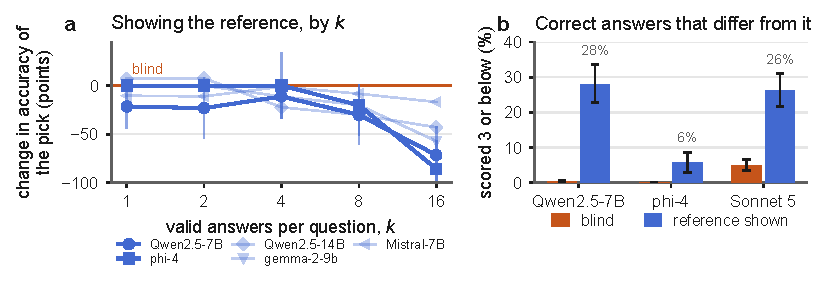
\includegraphics[width=\textwidth]{figures/fig2_selection.pdf}
\caption{\textbf{Selection accuracy by $k$ and false rejections, original scorer.} \textbf{(a)}~Change in the accuracy of the best-of-64 pick when the reference is shown, by the number of correct answers $k$ on the $k$-pool; Qwen2.5-7B and phi-4 in bold with 95\% intervals, three other judges light. \textbf{(b)}~Share of correct answers that differ from the reference scored 3 or below, blind (orange) and with the reference (blue), replication pool.\ph}
\label{fig:selection}
\end{figure}

\begin{table}[htbp]
\centering
\caption{$k$-pool: change in selection accuracy relative to blind judging, in percentage points (95\% CI). After the pass-rate filter, 14 tasks remain at $k{=}1$ and 39 in total at $k{>}1$ (7 at $k{=}16$). Interval bounds of exactly zero arise because per-task accuracy changes take few distinct values.\ph}
\label{tab:acc-kpool}
\footnotesize
\setlength{\tabcolsep}{3pt}
\begin{adjustbox}{max width=\linewidth}\begin{tabular}{llcccccc}
\toprule
Judge & Protocol & $k{=}1$ & $k{=}2$ & $k{=}4$ & $k{=}8$ & $k{=}16$ & pooled $k{>}1$ \\
\midrule
Qwen2.5-7B & reference & $-21.4$ & $-23.1$ & $-11.1$ & $-30.0$ & $-71.4$ & $-30.8$ \\
 & & {\scriptsize$[-43,+0]$} & {\scriptsize$[-54,+8]$} & {\scriptsize$[-33,+0]$} & {\scriptsize$[-60,+0]$} & {\scriptsize$[-100,-43]$} & {\scriptsize$[-46,-18]$} \\
 & blind, then reveal & $-21.4$ & $-15.4$ & $-11.1$ & $-10.0$ & $+0.0$ & $-10.3$ \\
 & & {\scriptsize$[-43,+0]$} & {\scriptsize$[-46,+16]$} & {\scriptsize$[-33,+0]$} & {\scriptsize$[-30,+0]$} & {\scriptsize$[-43,+43]$} & {\scriptsize$[-26,+5]$} \\
 & validity gate & $+0.0$ & $+15.4$ & $+0.0$ & $-10.0$ & $-28.6$ & $-2.6$ \\
 & & {\scriptsize$[+0,+0]$} & {\scriptsize$[+0,+38]$} & {\scriptsize$[+0,+0]$} & {\scriptsize$[-30,+0]$} & {\scriptsize$[-57,+0]$} & {\scriptsize$[-13,+8]$} \\
\addlinespace
phi-4 & reference & $+0.0$ & $+0.0$ & $+0.0$ & $-20.0$ & $-85.7$ & $-20.5$ \\
 & & {\scriptsize$[+0,+0]$} & {\scriptsize$[+0,+0]$} & {\scriptsize$[-33,+33]$} & {\scriptsize$[-50,+0]$} & {\scriptsize$[-100,-57]$} & {\scriptsize$[-36,-5]$} \\
 & blind, then reveal & $-14.3$ & $+0.0$ & $+0.0$ & $-20.0$ & $-57.1$ & $-15.4$ \\
 & & {\scriptsize$[-36,+0]$} & {\scriptsize$[+0,+0]$} & {\scriptsize$[-33,+33]$} & {\scriptsize$[-50,+0]$} & {\scriptsize$[-86,-14]$} & {\scriptsize$[-28,-3]$} \\
 & validity gate & $-7.1$ & $+0.0$ & $+0.0$ & $+0.0$ & $+0.0$ & $+0.0$ \\
 & & {\scriptsize$[-21,+0]$} & {\scriptsize$[+0,+0]$} & {\scriptsize$[+0,+0]$} & {\scriptsize$[+0,+0]$} & {\scriptsize$[+0,+0]$} & {\scriptsize$[+0,+0]$} \\
\addlinespace
Qwen2.5-14B & reference & $+7.1$ & $+7.7$ & $-22.2$ & $-30.0$ & $-42.9$ & $-17.9$ \\
 & & {\scriptsize$[-14,+29]$} & {\scriptsize$[+0,+23]$} & {\scriptsize$[-67,+22]$} & {\scriptsize$[-60,+0]$} & {\scriptsize$[-71,-14]$} & {\scriptsize$[-33,-3]$} \\
 & blind, then reveal & $+4.7$ & $+7.7$ & $+11.1$ & $+0.0$ & $-14.3$ & $+2.6$ \\
 & & {\scriptsize$[-4,+20]$} & {\scriptsize$[+0,+23]$} & {\scriptsize$[+0,+33]$} & {\scriptsize$[+0,+0]$} & {\scriptsize$[-43,+0]$} & {\scriptsize$[-5,+13]$} \\
 & validity gate & $+0.0$ & $+0.0$ & $+0.0$ & $+0.0$ & $-14.3$ & $-2.6$ \\
 & & {\scriptsize$[+0,+0]$} & {\scriptsize$[+0,+0]$} & {\scriptsize$[+0,+0]$} & {\scriptsize$[+0,+0]$} & {\scriptsize$[-43,+0]$} & {\scriptsize$[-8,+0]$} \\
\addlinespace
gemma-2-9b & reference & $+0.0$ & $+0.0$ & $-11.1$ & $-20.0$ & $-57.1$ & $-17.9$ \\
 & & {\scriptsize$[+0,+0]$} & {\scriptsize$[+0,+0]$} & {\scriptsize$[-33,+0]$} & {\scriptsize$[-40,+0]$} & {\scriptsize$[-86,-29]$} & {\scriptsize$[-31,-8]$} \\
 & blind, then reveal & $+0.0$ & $+0.0$ & $-11.1$ & $+0.0$ & $-57.1$ & $-12.8$ \\
 & & {\scriptsize$[+0,+0]$} & {\scriptsize$[+0,+0]$} & {\scriptsize$[-33,+0]$} & {\scriptsize$[+0,+0]$} & {\scriptsize$[-86,-29]$} & {\scriptsize$[-26,-3]$} \\
 & validity gate & $+0.0$ & $+0.0$ & $-11.1$ & $+0.0$ & $+0.0$ & $-2.6$ \\
 & & {\scriptsize$[+0,+0]$} & {\scriptsize$[+0,+0]$} & {\scriptsize$[-33,+0]$} & {\scriptsize$[+0,+0]$} & {\scriptsize$[+0,+0]$} & {\scriptsize$[-8,+0]$} \\
\addlinespace
Mistral-7B & reference & $-10.3$ & $-11.0$ & $-1.0$ & $-8.3$ & $-16.8$ & $-9.0$ \\
 & & {\scriptsize$[-15,-5]$} & {\scriptsize$[-16,-4]$} & {\scriptsize$[-5,+2]$} & {\scriptsize$[-14,-3]$} & {\scriptsize$[-25,-7]$} & {\scriptsize$[-12,-5]$} \\
 & blind, then reveal & $+0.6$ & $+1.3$ & $+1.3$ & $-1.6$ & $-2.8$ & $-0.1$ \\
 & & {\scriptsize$[-4,+5]$} & {\scriptsize$[-3,+8]$} & {\scriptsize$[+0,+3]$} & {\scriptsize$[-6,+3]$} & {\scriptsize$[-7,+2]$} & {\scriptsize$[-3,+3]$} \\
 & validity gate & $-29.4$ & $+7.1$ & $-45.5$ & $+1.3$ & $-18.7$ & $-11.2$ \\
 & & {\scriptsize$[-54,-6]$} & {\scriptsize$[-10,+19]$} & {\scriptsize$[-73,-13]$} & {\scriptsize$[-15,+17]$} & {\scriptsize$[-47,+10]$} & {\scriptsize$[-24,+1]$} \\
\bottomrule
\end{tabular}
\end{adjustbox}

\end{table}

\begin{table}[htbp]
\centering
\caption{Replication pool: selection accuracy on the 105 tasks in the pass-rate band, and false-rejection rate (correct answers that differ from the reference scored 3 or below) on the 93 tasks with both kinds of valid answer. Original scorer. Sonnet~5's selection accuracy cannot be computed: to save cost, only its scores for correct answers were collected.\ph}
\label{tab:acc-repl}
\footnotesize
\begin{adjustbox}{max width=\linewidth}\begin{tabular}{lcccc}
\toprule
Judge & Blind accuracy & With reference & Change (points) & False rejections, blind $\to$ reference \\
\midrule
Qwen2.5-7B & 76.2\% & 68.6\% & $-7.6$ {\scriptsize$[-19.1,+3.8]$} & 0.4\% $\to$ 28.0\% \\
phi-4 & 98.1\% & 86.7\% & $-11.4$ {\scriptsize$[-19.1,-4.8]$} & 0.0\% $\to$ 5.8\% \\
Claude Sonnet 5 & --- & --- & --- & 4.9\% $\to$ 26.2\% \\
\bottomrule
\end{tabular}
\end{adjustbox}

\end{table}

\begin{table}[htbp]
\centering
\caption{$k$-pool: added inflation over blind judging by $k$ (\sd, 95\% CI), 11 to 15 tasks per stratum.\osf}
\label{tab:kpool}
\footnotesize
\setlength{\tabcolsep}{3pt}
\begin{adjustbox}{max width=\linewidth}\begin{tabular}{lcccccc}
\toprule
 & \multicolumn{3}{c}{Qwen2.5-7B} & \multicolumn{3}{c}{phi-4} \\
\cmidrule(lr){2-4}\cmidrule(lr){5-7}
$k$ & reference & blind, then reveal & validity gate & reference & blind, then reveal & validity gate \\
\midrule
1 & \begin{tabular}[c]{@{}c@{}}$+0.05$\\{\scriptsize$[-0.30,+0.43]$}\end{tabular} & \begin{tabular}[c]{@{}c@{}}$+0.41$\\{\scriptsize$[-0.09,+0.84]$}\end{tabular} & \begin{tabular}[c]{@{}c@{}}$-0.04$\\{\scriptsize$[-0.30,+0.16]$}\end{tabular} & \begin{tabular}[c]{@{}c@{}}$-0.11$\\{\scriptsize$[-0.14,-0.07]$}\end{tabular} & \begin{tabular}[c]{@{}c@{}}$+0.04$\\{\scriptsize$[-0.13,+0.27]$}\end{tabular} & \begin{tabular}[c]{@{}c@{}}$+0.05$\\{\scriptsize$[-0.04,+0.21]$}\end{tabular} \\
2 & \begin{tabular}[c]{@{}c@{}}$+0.96$\\{\scriptsize$[+0.58,+1.34]$}\end{tabular} & \begin{tabular}[c]{@{}c@{}}$-0.30$\\{\scriptsize$[-0.92,+0.25]$}\end{tabular} & \begin{tabular}[c]{@{}c@{}}$+0.67$\\{\scriptsize$[+0.32,+0.99]$}\end{tabular} & \begin{tabular}[c]{@{}c@{}}$+0.58$\\{\scriptsize$[+0.29,+0.87]$}\end{tabular} & \begin{tabular}[c]{@{}c@{}}$+0.02$\\{\scriptsize$[-0.12,+0.16]$}\end{tabular} & \begin{tabular}[c]{@{}c@{}}$-0.07$\\{\scriptsize$[-0.11,-0.04]$}\end{tabular} \\
4 & \begin{tabular}[c]{@{}c@{}}$+1.77$\\{\scriptsize$[+0.96,+2.52]$}\end{tabular} & \begin{tabular}[c]{@{}c@{}}$+0.06$\\{\scriptsize$[-0.46,+0.58]$}\end{tabular} & \begin{tabular}[c]{@{}c@{}}$+1.15$\\{\scriptsize$[+0.34,+2.30]$}\end{tabular} & \begin{tabular}[c]{@{}c@{}}$+1.54$\\{\scriptsize$[+0.89,+2.19]$}\end{tabular} & \begin{tabular}[c]{@{}c@{}}$+0.08$\\{\scriptsize$[-0.31,+0.49]$}\end{tabular} & \begin{tabular}[c]{@{}c@{}}$-0.10$\\{\scriptsize$[-0.16,-0.06]$}\end{tabular} \\
8 & \begin{tabular}[c]{@{}c@{}}$+1.90$\\{\scriptsize$[+1.26,+2.48]$}\end{tabular} & \begin{tabular}[c]{@{}c@{}}$+0.12$\\{\scriptsize$[-0.27,+0.51]$}\end{tabular} & \begin{tabular}[c]{@{}c@{}}$+1.00$\\{\scriptsize$[+0.58,+1.51]$}\end{tabular} & \begin{tabular}[c]{@{}c@{}}$+0.99$\\{\scriptsize$[+0.40,+1.60]$}\end{tabular} & \begin{tabular}[c]{@{}c@{}}$+0.18$\\{\scriptsize$[-0.20,+0.50]$}\end{tabular} & \begin{tabular}[c]{@{}c@{}}$+0.03$\\{\scriptsize$[-0.09,+0.15]$}\end{tabular} \\
16 & \begin{tabular}[c]{@{}c@{}}$+1.39$\\{\scriptsize$[+0.71,+2.05]$}\end{tabular} & \begin{tabular}[c]{@{}c@{}}$-0.06$\\{\scriptsize$[-0.61,+0.56]$}\end{tabular} & \begin{tabular}[c]{@{}c@{}}$+2.77$\\{\scriptsize$[+1.75,+3.89]$}\end{tabular} & \begin{tabular}[c]{@{}c@{}}$+1.28$\\{\scriptsize$[+0.89,+1.69]$}\end{tabular} & \begin{tabular}[c]{@{}c@{}}$+0.44$\\{\scriptsize$[+0.13,+0.76]$}\end{tabular} & \begin{tabular}[c]{@{}c@{}}$-0.15$\\{\scriptsize$[-0.21,-0.10]$}\end{tabular} \\
\midrule
pooled $>1$ & \begin{tabular}[c]{@{}c@{}}$+1.50$\\{\scriptsize$[+1.17,+1.82]$}\end{tabular} & \begin{tabular}[c]{@{}c@{}}$-0.05$\\{\scriptsize$[-0.32,+0.21]$}\end{tabular} & \begin{tabular}[c]{@{}c@{}}$+1.31$\\{\scriptsize$[+0.91,+1.77]$}\end{tabular} & \begin{tabular}[c]{@{}c@{}}$+1.07$\\{\scriptsize$[+0.81,+1.34]$}\end{tabular} & \begin{tabular}[c]{@{}c@{}}$+0.16$\\{\scriptsize$[+0.00,+0.33]$}\end{tabular} & \begin{tabular}[c]{@{}c@{}}$-0.07$\\{\scriptsize$[-0.11,-0.03]$}\end{tabular} \\
\bottomrule
\end{tabular}
\end{adjustbox}

\end{table}

\begin{table}[htbp]
\centering
\caption{Synthetic grid, Qwen-generated pool: added inflation (\sd, 95\% CI). After filtering, 6 tasks remain at $k{=}1$ and 20 task-strata over $k{>}1$. The step is positive for all six judges; the level pooled over $k{>}1$ is individually significant for three. Post-hoc paired re-analysis of a pre-specified grid.}
\label{tab:grid}
\footnotesize
\setlength{\tabcolsep}{4pt}
\begin{adjustbox}{max width=\linewidth}\begin{tabular}{lcccc}
\toprule
Judge & At $k{=}1$ & Pooled $k{>}1$ & Step & Slope per doubling of $k$ \\
\midrule
Qwen2.5-1.5B & $-0.48$ {\scriptsize$[-0.70,-0.29]$} & $+0.07$ {\scriptsize$[-0.15,+0.26]$} & $+0.55$ {\scriptsize$[+0.26,+0.85]$} & $+0.02$ {\scriptsize$[-0.20,+0.18]$} \\
Qwen2.5-3B & $-0.14$ {\scriptsize$[-0.30,-0.03]$} & $+2.41$ {\scriptsize$[+1.40,+3.49]$} & $+2.55$ {\scriptsize$[+1.50,+3.67]$} & $-0.06$ {\scriptsize$[-1.04,+1.06]$} \\
Qwen2.5-7B & $-0.33$ {\scriptsize$[-0.53,-0.11]$} & $+0.89$ {\scriptsize$[+0.45,+1.37]$} & $+1.22$ {\scriptsize$[+0.70,+1.73]$} & $+0.28$ {\scriptsize$[-0.10,+0.64]$} \\
Qwen2.5-14B & $-0.38$ {\scriptsize$[-0.56,-0.19]$} & $+0.08$ {\scriptsize$[-0.20,+0.36]$} & $+0.46$ {\scriptsize$[+0.13,+0.80]$} & $+0.23$ {\scriptsize$[+0.00,+0.46]$} \\
Llama-3.1-8B & $-0.28$ {\scriptsize$[-0.65,+0.07]$} & $+0.46$ {\scriptsize$[+0.12,+0.79]$} & $+0.73$ {\scriptsize$[+0.25,+1.24]$} & $+0.36$ {\scriptsize$[+0.07,+0.65]$} \\
phi-4 & $-0.58$ {\scriptsize$[-0.86,-0.30]$} & $+0.22$ {\scriptsize$[-0.19,+0.65]$} & $+0.80$ {\scriptsize$[+0.30,+1.28]$} & $+0.37$ {\scriptsize$[+0.06,+0.70]$} \\
\bottomrule
\end{tabular}
\end{adjustbox}

\end{table}

\begin{figure}[htbp]
\centering
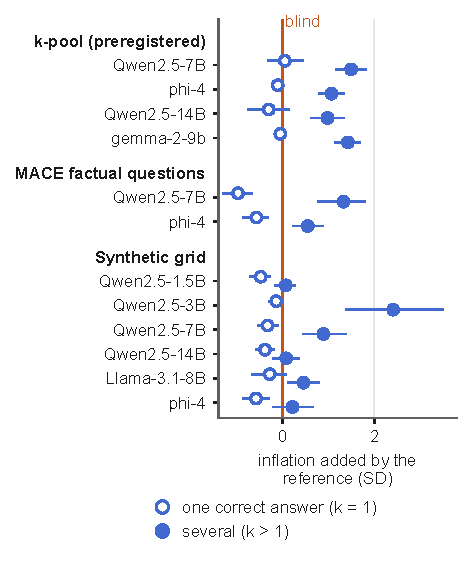
\includegraphics[width=0.6\textwidth]{figures/fig2_boundary.pdf}
\caption{\textbf{The inflation the reference adds is higher with several correct answers than with one.} Per task, referenced minus blind (\sd, 95\% intervals), for tasks with one correct answer (hollow) and several (filled); registered labels. $k$-pool and coverage judges: preregistered.\osf{} \textsc{MACE}: factual questions.\pre{} Synthetic grid: a paired re-analysis of the pre-specified grid.\ph{} Because every correct answer matches the reference when $k{=}1$, the step follows from the swap result and is not an independent test.}
\label{fig:boundary}
\end{figure}

\begin{figure}[htbp]
\centering
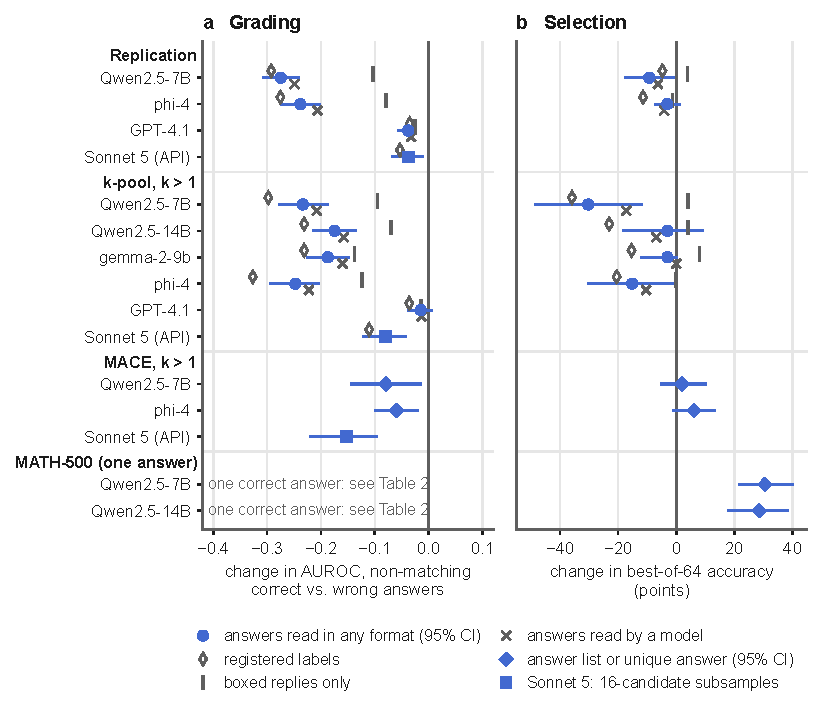
\includegraphics[width=0.94\textwidth]{figures/fig3_cost.pdf}
\caption{\textbf{Grading and selection under three ways of reading answers.} Referenced minus blind, per task. Blue circles: answers read in any format, 95\% intervals; grey diamonds: registered labels; grey ticks: boxed replies only; grey crosses: answers read by a model; blue diamonds: \textsc{MACE}'s answer lists and MATH-500's unique answers; blue squares: Sonnet~5 on 16-candidate subsamples. \textbf{(a)}~Change in grading AUROC for correct answers that differ from the reference against wrong answers. \textbf{(b)}~Change in best-of-64 accuracy; not shown for Sonnet~5, whose subsamples always contain a correct answer matching the reference, or GPT-4.1, whose scores tie. Exact scorer for Qwen2.5 and gemma-2. Any-format and model-read values for open judges are post hoc.\ph}
\label{fig:cost}
\end{figure}

\paragraph{Reading answers in any format.}
The registered checkers read an answer from its \texttt{\textbackslash boxed\{\}} content. On the $k$-pool a reply without a box is compared as a whole, and on the replication pool the checker needs exactly one integer in the reply's last 100 characters, so most answers stated in prose count as wrong. Only 61.6\% of replication samples and 57.1\% of $k$-pool samples use the box.
We relabeled every reply post hoc, before reading any judge score with the new labels. The extracted answer is the boxed content if there is one; otherwise it is the last integer in the reply for tasks with a one-integer answer, and the integers of the reply's last stated clause for subset-sum and Goldbach tasks. A reply counts as correct if the registered checker accepts it or the task's constraint accepts the extracted answer. In a second labeling, Qwen2.5-14B-Instruct reads each unboxed reply and reports the final answer it commits to, or none; 54\% and 55\% of unboxed replies commit to none. The rule relabels 695 replication and 444 $k$-pool candidates as correct, the model somewhat more, and the two agree on 88\% of unboxed replies (\cref{tab:labelings-numbers}). In a spot check of 30 replies the rule relabeled, 3 were doubtful: a hedged pair of answers or a truncated list of candidates. A registered audit then had Claude Opus~5 (API, thinking disabled, the same extraction prompt) read a stratified random sample of 200 unboxed replies, 50 per pool and any-format label, and labeled each with the constraint check applied to the answer it reported. Weighted by stratum sizes, its reading agrees with the any-format label on 91.1\% of unboxed replies (predicted at least 85\%; confirmed) and with the Qwen2.5-14B reading on 94.7\%. It confirms 86.2\% of the replies the any-format rule credits (predicted at least 90\%; falsified) and credits 7.4\% of those the rule rejects (predicted at most 15\%; confirmed). Of the 13 sampled replies the rule credits and the reader does not, 6 end by listing several numbers, whose last integer the rule takes as the answer, 5 commit to no answer, and 2 are single integers the constraint check rejects; of the 8 the rule rejects and the reader credits, 6 are subset-sum or Goldbach answers in an order or format the rule misparses. The any-format labels therefore over-credit some replies, which is one reason we also report boxed replies alone.
\Cref{tab:labelings-acc,tab:labelings-gnm,tab:labelings-fr} report selection accuracy, grading AUROC for correct non-matching against wrong answers, and false rejections under the registered labels, both relabelings, and the registered labels restricted to boxed replies. Grading gets worse under the registered labels and both relabelings for every open judge; keeping only boxed replies shrinks the fall to 0.07 to 0.14 and removes it for Mistral-7B, whose integer scores failed our score-resolution screen. Under the registered labels and the exact scorer, Qwen2.5-7B scores 28.1\% of the replication
pool's correct answers that differ from the reference 3 or below with the reference, against 0.4\%
blind (93 tasks).\pre{} The selection loss at $k{>}1$ does not survive in the same way: crediting answers in any format leaves a loss that excludes zero only for Qwen2.5-7B, and with model-read labels no loss excludes zero. The preregistered inflation endpoints do survive relabeling (\cref{tab:inflation-relabeled}): on the replication pool the pooled endpoint is $+1.19$ under the registered labels, $+1.14$ with answers read in any format, and $+1.12$ with model-read labels, and on the $k$-pool at $k{>}1$ the reference adds $+1.44$ and $+0.98$ with any-format labels against $+1.50$ and $+1.06$ registered. At $k{=}1$ the relabeling changes the sign: with answers read in any format the reference lowers inflation for both $k$-pool judges ($-0.27$ and $-0.15$), as the answer-key reading predicts for a single correct answer. An earlier version of this analysis instead set aside wrong candidates that contain the reference's answer (\cref{tab:round7}); most of those were unboxed replies stating a correct value, which the relabelings count as correct.\ph

\begin{table}[htbp]
\centering
\caption{Change in best-of-64 accuracy from showing the reference (points, 95\% CI), constructed pools, under four labelings. The pass-rate band is recomputed under each labeling. Exact scorer for Qwen2.5 and gemma-2; Mistral-7B's scores are parsed integers. Registered-checker values for the four open $k$-pool judges at $k{>}1$ are a pre-specified re-analysis ($\ddagger$); the rest are post hoc.}
\label{tab:labelings-acc}
\footnotesize
\setlength{\tabcolsep}{3pt}
\begin{adjustbox}{max width=\linewidth}\begin{tabular}{llcccc}
\toprule
Pool & Judge & Registered & Any format & Model-read & Boxed only \\
\midrule
Replication & Qwen2.5-7B & $-4.8$ {\scriptsize$[-15.2,+5.7]$} & $-9.3$ {\scriptsize$[-17.5,-1.0]$} & $-6.3$ {\scriptsize$[-13.7,+1.1]$} & $+3.9$ {\scriptsize$[-1.3,+9.1]$} \\
 & phi-4 & $-11.4$ {\scriptsize$[-19.1,-4.8]$} & $-3.1$ {\scriptsize$[-7.2,+1.0]$} & $-4.2$ {\scriptsize$[-9.5,+1.1]$} & $-1.3$ {\scriptsize$[-6.5,+2.6]$} \\
 & GPT-4.1 & $+0.1$ {\scriptsize$[-2.9,+3.2]$} & $-0.3$ {\scriptsize$[-3.1,+2.2]$} & $+1.2$ {\scriptsize$[-0.1,+3.0]$} & $+0.7$ {\scriptsize$[-0.5,+2.5]$} \\
\addlinespace
$k$-pool, $k{=}1$ & Qwen2.5-7B & $-21.4$ {\scriptsize$[-42.9,+0.0]$} & $+0.0$ {\scriptsize$[+0.0,+0.0]$} & $+0.0$ {\scriptsize$[+0.0,+0.0]$} & $+0.0$ {\scriptsize$[+0.0,+0.0]$} \\
 & Qwen2.5-14B & $+3.6$ {\scriptsize$[-21.4,+28.6]$} & $+0.0$ {\scriptsize$[+0.0,+0.0]$} & $+0.0$ {\scriptsize$[+0.0,+0.0]$} & $+0.0$ {\scriptsize$[+0.0,+0.0]$} \\
 & gemma-2-9b & $+0.0$ {\scriptsize$[+0.0,+0.0]$} & $+0.0$ {\scriptsize$[+0.0,+0.0]$} & $+0.0$ {\scriptsize$[+0.0,+0.0]$} & $+0.0$ {\scriptsize$[+0.0,+0.0]$} \\
 & phi-4 & $+0.0$ {\scriptsize$[+0.0,+0.0]$} & $+0.0$ {\scriptsize$[+0.0,+0.0]$} & $+0.0$ {\scriptsize$[+0.0,+0.0]$} & $+0.0$ {\scriptsize$[+0.0,+0.0]$} \\
 & Mistral-7B & $-10.4$ {\scriptsize$[-16.1,-4.4]$} & $-3.3$ {\scriptsize$[-7.9,+0.6]$} & $-2.8$ {\scriptsize$[-6.9,+1.2]$} & $-4.6$ {\scriptsize$[-10.6,+1.4]$} \\
 & GPT-4.1 & $+4.0$ {\scriptsize$[-6.2,+18.8]$} & $-0.1$ {\scriptsize$[-0.7,+0.4]$} & $+0.0$ {\scriptsize$[+0.0,+0.0]$} & $+0.0$ {\scriptsize$[+0.0,+0.0]$} \\
\addlinespace
$k$-pool, $k{>}1$ & Qwen2.5-7B & $-35.9$ {\scriptsize$[-51.3,-20.5]$} & $-30.3$ {\scriptsize$[-48.5,-12.1]$} & $-17.2$ {\scriptsize$[-34.5,+3.5]$} & $+4.0$ {\scriptsize$[-20.0,+28.0]$} \\
 & Qwen2.5-14B & $-23.1$ {\scriptsize$[-38.5,-7.7]$} & $-3.0$ {\scriptsize$[-18.2,+9.1]$} & $-6.9$ {\scriptsize$[-20.7,+6.9]$} & $+4.0$ {\scriptsize$[-12.0,+20.0]$} \\
 & gemma-2-9b & $-15.4$ {\scriptsize$[-28.2,-5.1]$} & $-3.0$ {\scriptsize$[-12.1,+0.0]$} & $+0.0$ {\scriptsize$[-10.3,+10.3]$} & $+8.0$ {\scriptsize$[-4.0,+24.0]$} \\
 & phi-4 & $-20.5$ {\scriptsize$[-35.9,-5.1]$} & $-15.2$ {\scriptsize$[-30.3,+0.0]$} & $-10.3$ {\scriptsize$[-27.6,+6.9]$} & $+0.0$ {\scriptsize$[-16.0,+16.0]$} \\
 & Mistral-7B & $-8.5$ {\scriptsize$[-11.8,-4.7]$} & $-4.7$ {\scriptsize$[-8.6,-0.8]$} & $-2.8$ {\scriptsize$[-6.8,+1.5]$} & $+1.6$ {\scriptsize$[-4.5,+7.5]$} \\
 & GPT-4.1 & $-1.6$ {\scriptsize$[-7.6,+3.5]$} & $+0.8$ {\scriptsize$[-8.5,+10.1]$} & $+2.5$ {\scriptsize$[-7.1,+12.7]$} & $+12.5$ {\scriptsize$[+3.3,+24.3]$} \\
\bottomrule
\end{tabular}
\end{adjustbox}
\end{table}

\begin{table}[htbp]
\centering
\caption{Change in per-task AUROC for separating correct answers that differ from the reference from wrong answers (95\% CI), under four labelings. Exact scorer for Qwen2.5 and gemma-2; matches are decided from the extracted answer (compare \cref{tab:r4-grading}). Qwen2.5-7B's replication value under the registered checker is pre-specified; the rest are post hoc.}
\label{tab:labelings-gnm}
\footnotesize
\setlength{\tabcolsep}{3pt}
\begin{adjustbox}{max width=\linewidth}\begin{tabular}{llcccc}
\toprule
Pool & Judge & Registered & Any format & Model-read & Boxed only \\
\midrule
Replication & Qwen2.5-7B & $-0.29$ {\scriptsize$[-0.32,-0.26]$} & $-0.27$ {\scriptsize$[-0.31,-0.24]$} & $-0.25$ {\scriptsize$[-0.28,-0.22]$} & $-0.10$ {\scriptsize$[-0.13,-0.08]$} \\
 & phi-4 & $-0.28$ {\scriptsize$[-0.31,-0.25]$} & $-0.24$ {\scriptsize$[-0.27,-0.20]$} & $-0.21$ {\scriptsize$[-0.24,-0.18]$} & $-0.08$ {\scriptsize$[-0.10,-0.06]$} \\
 & GPT-4.1 & $-0.04$ {\scriptsize$[-0.05,-0.02]$} & $-0.04$ {\scriptsize$[-0.06,-0.02]$} & $-0.03$ {\scriptsize$[-0.05,-0.02]$} & $-0.02$ {\scriptsize$[-0.04,-0.01]$} \\
\addlinespace
$k$-pool, $k{>}1$ & Qwen2.5-7B & $-0.30$ {\scriptsize$[-0.34,-0.25]$} & $-0.23$ {\scriptsize$[-0.28,-0.19]$} & $-0.21$ {\scriptsize$[-0.26,-0.16]$} & $-0.09$ {\scriptsize$[-0.15,-0.04]$} \\
 & Qwen2.5-14B & $-0.23$ {\scriptsize$[-0.28,-0.19]$} & $-0.17$ {\scriptsize$[-0.21,-0.14]$} & $-0.16$ {\scriptsize$[-0.20,-0.12]$} & $-0.07$ {\scriptsize$[-0.10,-0.04]$} \\
 & gemma-2-9b & $-0.23$ {\scriptsize$[-0.27,-0.19]$} & $-0.19$ {\scriptsize$[-0.23,-0.15]$} & $-0.16$ {\scriptsize$[-0.20,-0.12]$} & $-0.14$ {\scriptsize$[-0.19,-0.09]$} \\
 & phi-4 & $-0.33$ {\scriptsize$[-0.38,-0.27]$} & $-0.25$ {\scriptsize$[-0.29,-0.20]$} & $-0.22$ {\scriptsize$[-0.27,-0.17]$} & $-0.12$ {\scriptsize$[-0.18,-0.07]$} \\
 & Mistral-7B & $-0.10$ {\scriptsize$[-0.13,-0.06]$} & $-0.08$ {\scriptsize$[-0.11,-0.05]$} & $-0.08$ {\scriptsize$[-0.12,-0.04]$} & $+0.01$ {\scriptsize$[-0.05,+0.07]$} \\
 & GPT-4.1 & $-0.04$ {\scriptsize$[-0.08,-0.01]$} & $-0.01$ {\scriptsize$[-0.04,+0.00]$} & $-0.01$ {\scriptsize$[-0.03,+0.00]$} & $-0.01$ {\scriptsize$[-0.06,+0.02]$} \\
\bottomrule
\end{tabular}
\end{adjustbox}
\end{table}

\begin{table}[htbp]
\centering
\caption{Change in the share of correct non-matching answers scored 3 or below (points, 95\% CI), under four labelings. Exact scorer for Qwen2.5 and gemma-2; matches are decided from the extracted answer.\ph}
\label{tab:labelings-fr}
\footnotesize
\setlength{\tabcolsep}{3pt}
\begin{adjustbox}{max width=\linewidth}\begin{tabular}{llcccc}
\toprule
Pool & Judge & Registered & Any format & Model-read & Boxed only \\
\midrule
Replication & Qwen2.5-7B & $+28.2$ {\scriptsize$[+23.6,+33.2]$} & $+27.0$ {\scriptsize$[+22.5,+31.8]$} & $+25.9$ {\scriptsize$[+21.7,+30.5]$} & $+28.3$ {\scriptsize$[+23.6,+33.2]$} \\
 & phi-4 & $+6.8$ {\scriptsize$[+4.5,+9.9]$} & $+6.6$ {\scriptsize$[+4.4,+9.2]$} & $+6.5$ {\scriptsize$[+4.3,+9.0]$} & $+6.8$ {\scriptsize$[+4.5,+9.7]$} \\
 & GPT-4.1 & $+5.8$ {\scriptsize$[+3.5,+8.6]$} & $+6.4$ {\scriptsize$[+4.0,+9.1]$} & $+6.4$ {\scriptsize$[+4.2,+9.0]$} & $+6.0$ {\scriptsize$[+3.5,+8.7]$} \\
\addlinespace
$k$-pool, $k{>}1$ & Qwen2.5-7B & $+35.4$ {\scriptsize$[+28.3,+42.4]$} & $+32.4$ {\scriptsize$[+26.2,+38.5]$} & $+32.3$ {\scriptsize$[+25.6,+39.0]$} & $+35.4$ {\scriptsize$[+28.3,+42.4]$} \\
 & Qwen2.5-14B & $+14.4$ {\scriptsize$[+8.9,+20.2]$} & $+13.4$ {\scriptsize$[+8.3,+19.4]$} & $+13.1$ {\scriptsize$[+8.2,+18.7]$} & $+14.4$ {\scriptsize$[+8.9,+20.2]$} \\
 & gemma-2-9b & $+54.4$ {\scriptsize$[+46.8,+62.1]$} & $+52.8$ {\scriptsize$[+44.9,+60.5]$} & $+51.8$ {\scriptsize$[+45.6,+58.5]$} & $+53.7$ {\scriptsize$[+45.7,+61.7]$} \\
 & phi-4 & $+11.7$ {\scriptsize$[+7.4,+16.5]$} & $+10.3$ {\scriptsize$[+6.2,+14.8]$} & $+9.5$ {\scriptsize$[+5.9,+13.4]$} & $+12.6$ {\scriptsize$[+7.8,+18.1]$} \\
 & Mistral-7B & $+4.9$ {\scriptsize$[+1.5,+9.6]$} & $+6.9$ {\scriptsize$[+2.5,+11.8]$} & $+6.6$ {\scriptsize$[+1.7,+11.6]$} & $+4.8$ {\scriptsize$[+1.6,+9.5]$} \\
 & GPT-4.1 & $+1.0$ {\scriptsize$[-4.0,+6.0]$} & $+1.2$ {\scriptsize$[-2.4,+4.8]$} & $+0.0$ {\scriptsize$[-3.6,+3.9]$} & $+1.0$ {\scriptsize$[-4.0,+6.0]$} \\
\bottomrule
\end{tabular}
\end{adjustbox}
\end{table}

\begin{table}[htbp]
\centering
\caption{Labeling counts, agreement between the rule and the model on unboxed replies, and $k$-pool selection at $k{>}1$ with answers read in any format for the referenced judge, the max rule, and blind-then-reveal (original scorer for all three, so the reference row differs from \cref{tab:labelings-acc}).\ph}
\label{tab:labelings-numbers}
\footnotesize
\begin{adjustbox}{max width=\linewidth}\begin{tabular}{L{7.6cm}L{5.4cm}}
\toprule
Quantity & Value \\
\midrule
Replication pool: samples; with a \texttt{\textbackslash boxed\{\}} answer & 7680; 4730 (61.6\%) \\
Replication pool: correct under the registered checker; in any format & 3494; 4189 (+682 unboxed, +13 boxed) \\
$k$-pool: samples; with a \texttt{\textbackslash boxed\{\}} answer & 4800; 2739 (57.1\%) \\
$k$-pool: correct under the registered checker; in any format & 1926; 2370 (+431 unboxed, +13 boxed) \\
Replication pool, unboxed replies: rule and model labels agree; correct by rule / by model & 87.9\%; 760 / 925 \\
$k$-pool, unboxed replies: rule and model labels agree; correct by rule / by model & 88.4\%; 453 / 594 \\
$k$-pool, $k{>}1$, any format, Qwen2.5-7B: accuracy change for reference; max rule; blind, then reveal (points) & $-24.2$ {\scriptsize$[-42.4,-6.1]$}; $+3.0$ {\scriptsize$[+0.0,+9.1]$}; $+0.0$ {\scriptsize$[-12.1,+12.1]$} \\
$k$-pool, $k{>}1$, any format, Qwen2.5-14B: accuracy change for reference; max rule; blind, then reveal (points) & $+0.0$ {\scriptsize$[-12.1,+12.1]$}; $+3.0$ {\scriptsize$[-6.1,+12.1]$}; $+3.0$ {\scriptsize$[-6.1,+12.1]$} \\
$k$-pool, $k{>}1$, any format, gemma-2-9b: accuracy change for reference; max rule; blind, then reveal (points) & $-3.0$ {\scriptsize$[-12.1,+0.0]$}; $+0.0$ {\scriptsize$[+0.0,+0.0]$}; $+0.0$ {\scriptsize$[+0.0,+0.0]$} \\
$k$-pool, $k{>}1$, any format, phi-4: accuracy change for reference; max rule; blind, then reveal (points) & $-15.2$ {\scriptsize$[-30.3,+0.0]$}; $+3.0$ {\scriptsize$[+0.0,+9.1]$}; $-6.1$ {\scriptsize$[-18.2,+6.1]$} \\
\bottomrule
\end{tabular}
\end{adjustbox}
\end{table}

\begin{table}[htbp]
\centering
\caption{The preregistered inflation endpoints recomputed with the same estimator under corrected labels (\sd, 95\% CI). Replication: per-task referenced-minus-blind inflation on the registered 105 tasks, pooled over both judges by task-cluster bootstrap; the ``band recomputed'' row re-selects tasks with pass rate in $[0.2, 0.8]$ under each labeling. $k$-pool: condition minus blind on the registered tasks. The registered column reproduces the registered values up to tie-break and permutation randomness.\ph}
\label{tab:inflation-relabeled}
\footnotesize
\setlength{\tabcolsep}{3pt}
\begin{adjustbox}{max width=\linewidth}\begin{tabular}{llccc}
\toprule
Endpoint & Judge & Registered & Any format & Model-read \\
\midrule
Replication, 105 tasks & Qwen2.5-7B & $+1.29$ {\scriptsize$[+1.07,+1.52]$} & $+1.36$ {\scriptsize$[+1.16,+1.57]$} & $+1.34$ {\scriptsize$[+1.13,+1.56]$} \\
 & phi-4 & $+1.08$ {\scriptsize$[+0.94,+1.24]$} & $+0.92$ {\scriptsize$[+0.78,+1.05]$} & $+0.90$ {\scriptsize$[+0.77,+1.04]$} \\
 & Pooled & $+1.19$ {\scriptsize$[+1.02,+1.36]$} & $+1.14$ {\scriptsize$[+0.98,+1.29]$} & $+1.12$ {\scriptsize$[+0.97,+1.28]$} \\
 & Pooled, band recomputed & --- & $+1.10$ {\scriptsize$[+0.95,+1.26]$} & $+1.11$ {\scriptsize$[+0.95,+1.29]$} \\
\addlinespace
$k$-pool, reference, $k{=}1$ & Qwen2.5-7B & $+0.05$ {\scriptsize$[-0.30,+0.42]$} & $-0.27$ {\scriptsize$[-0.54,-0.04]$} & $-0.28$ {\scriptsize$[-0.54,-0.03]$} \\
 & phi-4 & $-0.11$ {\scriptsize$[-0.15,-0.08]$} & $-0.14$ {\scriptsize$[-0.19,-0.10]$} & $-0.19$ {\scriptsize$[-0.23,-0.14]$} \\
$k$-pool, reference, $k{>}1$ & Qwen2.5-7B & $+1.50$ {\scriptsize$[+1.16,+1.82]$} & $+1.44$ {\scriptsize$[+1.14,+1.74]$} & $+1.34$ {\scriptsize$[+1.02,+1.68]$} \\
 & phi-4 & $+1.06$ {\scriptsize$[+0.79,+1.34]$} & $+0.98$ {\scriptsize$[+0.73,+1.24]$} & $+0.85$ {\scriptsize$[+0.58,+1.12]$} \\
$k$-pool, blind, then reveal, $k{=}1$ & Qwen2.5-7B & $+0.41$ {\scriptsize$[-0.09,+0.83]$} & $+0.14$ {\scriptsize$[-0.26,+0.46]$} & $+0.03$ {\scriptsize$[-0.34,+0.25]$} \\
 & phi-4 & $+0.04$ {\scriptsize$[-0.14,+0.28]$} & $-0.16$ {\scriptsize$[-0.21,-0.12]$} & $-0.20$ {\scriptsize$[-0.25,-0.15]$} \\
$k$-pool, blind, then reveal, $k{>}1$ & Qwen2.5-7B & $-0.05$ {\scriptsize$[-0.31,+0.21]$} & $-0.11$ {\scriptsize$[-0.34,+0.12]$} & $-0.13$ {\scriptsize$[-0.36,+0.11]$} \\
 & phi-4 & $+0.15$ {\scriptsize$[-0.01,+0.33]$} & $+0.01$ {\scriptsize$[-0.12,+0.13]$} & $-0.04$ {\scriptsize$[-0.17,+0.08]$} \\
\bottomrule
\end{tabular}
\end{adjustbox}
\end{table}

\begin{table}[htbp]
\centering
\footnotesize
\caption{Robustness numbers: look-alike wrong answers, results with them removed, GPT-4.1 selection, Sonnet~5 score coverage, and Sonnet~5's mean scores of correct replication-pool answers (95\% CI).\ph}
\label{tab:round7}
\begin{adjustbox}{max width=\linewidth}\begin{tabular}{L{8.4cm}L{4.8cm}}
\toprule
Quantity & Value (95\% CI) \\
\midrule
\multicolumn{2}{l}{\emph{Wrong candidates whose text contains the reference's answer (look-alikes)}} \\
Replication pool: share of wrong candidates; share of those with no \texttt{\textbackslash boxed\{\}} answer & 23.6\%; 73.3\% \\
$k$-pool: share of wrong candidates; share of those with no \texttt{\textbackslash boxed\{\}} answer & 26.8\%; 76.9\% \\
\textsc{MACE} River and Language: share of wrong candidates & 3.1\% \\
\multicolumn{2}{l}{\emph{$k$-pool accuracy change with look-alikes removed (points): $k{=}1$; $k{>}1$; step}} \\
Qwen2.5-7B & $+0.0$ {\scriptsize$[+0.0,+0.0]$}; $-15.4$ {\scriptsize$[-28.2,-2.6]$}; step $-15.4$ {\scriptsize$[-28.2,-2.6]$} \\
Qwen2.5-14B & $+7.1$ {\scriptsize$[+0.0,+21.4]$}; $-5.1$ {\scriptsize$[-15.4,+5.1]$}; step $-12.3$ {\scriptsize$[-31.7,+2.6]$} \\
gemma-2-9b & $+0.0$ {\scriptsize$[+0.0,+0.0]$}; $-15.4$ {\scriptsize$[-28.2,-5.1]$}; step $-15.4$ {\scriptsize$[-28.2,-5.1]$} \\
phi-4 & $+0.0$ {\scriptsize$[+0.0,+0.0]$}; $-20.5$ {\scriptsize$[-35.9,-5.1]$}; step $-20.5$ {\scriptsize$[-35.9,-7.6]$} \\
\multicolumn{2}{l}{\emph{Replication pool with look-alikes removed: AUROC change (non-matching, all); accuracy change (points)}} \\
Qwen2.5-7B & $-0.24$ {\scriptsize$[-0.27,-0.21]$}, $-0.19$ {\scriptsize$[-0.22,-0.16]$}; $+1.9$ {\scriptsize$[-5.7,+9.5]$} \\
phi-4 & $-0.20$ {\scriptsize$[-0.23,-0.17]$}, $-0.16$ {\scriptsize$[-0.19,-0.13]$}; $-5.7$ {\scriptsize$[-11.4,-0.9]$} \\
\textsc{MACE}, Qwen2.5-7B, non-matching AUROC change with look-alikes removed & $-0.07$ {\scriptsize$[-0.14,-0.01]$} \\
\multicolumn{2}{l}{\emph{GPT-4.1 on the $k$-pool: accuracy change (points) and mean candidates tied at the maximum, blind / reference}} \\
GPT-4.1, $k{=}1$ & $+4.0$ {\scriptsize$[-6.2,+18.8]$}; ties 13.4 / 23.4 \\
GPT-4.1, $k{>}1$ & $-1.6$ {\scriptsize$[-7.6,+3.5]$}; ties 9.2 / 15.5 \\
Sonnet~5 score files, replication pool: correct answers scored; wrong answers scored & 3494 of 3494; 0 of 4186 \\
\multicolumn{2}{l}{\emph{Sonnet~5 (API) mean score of correct answers, replication pool, blind $\to$ reference}} \\
Matching the reference & 9.19 {\scriptsize$[+8.90,+9.45]$} $\to$ 9.99 {\scriptsize$[+9.98,+10.00]$} \\
Differing from the reference & 9.09 {\scriptsize$[+8.91,+9.26]$} $\to$ 6.93 {\scriptsize$[+6.39,+7.44]$} \\
\bottomrule
\end{tabular}
\end{adjustbox}
\end{table}

\paragraph{Robustness of the replication endpoint.}
Only 61.6\% of samples put their answer in the requested \texttt{\textbackslash boxed\{\}} format. Restricting to the top third of tasks by format compliance still gives $+0.90$, and including all 120 tasks rather than the 105 in the band gives $+1.14$ (\cref{tab:repl-robust}). The paired raw gap $G$, without the permutation adjustment, is already present at best-of-2 and grows with $n$ (\cref{tab:repl-pressure}).

\begin{table}[htbp]
\centering
\caption{Added inflation on the replication pool under different populations (\sd, 95\% CI). All rows except the first are post hoc.}
\label{tab:repl-robust}
\footnotesize
\begin{adjustbox}{max width=\linewidth}\begin{tabular}{lccc}
\toprule
Population & Qwen2.5-7B & phi-4 & Pooled \\
\midrule
Preregistered band (primary), 105 tasks & $+1.29$ {\scriptsize$[+1.06,+1.52]$} & $+1.09$ {\scriptsize$[+0.95,+1.24]$} & $+1.19$ {\scriptsize$[+1.03,+1.35]$} \\
All 120 tasks (intention to treat) & $+1.27$ {\scriptsize$[+1.06,+1.49]$} & $+1.01$ {\scriptsize$[+0.86,+1.17]$} & $+1.14$ {\scriptsize$[+0.97,+1.30]$} \\
15 out-of-band tasks only & $+1.13$ {\scriptsize$[+0.38,+1.81]$} & $+0.43$ {\scriptsize$[-0.09,+0.91]$} & $+0.78$ {\scriptsize$[+0.19,+1.32]$} \\
Top tercile of answer-format compliance, 40 tasks & & & $+0.90$ {\scriptsize$[+0.65,+1.16]$} \\
\bottomrule
\end{tabular}
\end{adjustbox}

\end{table}

\begin{table}[htbp]
\centering
\caption{Referenced-minus-blind raw gap $G$ by best-of-$n$ budget, pooled over both judges, 105 tasks.\ph}
\label{tab:repl-pressure}
\footnotesize
\begin{adjustbox}{max width=\linewidth}\begin{tabular}{lcccccc}
\toprule
Best-of-$n$ & $n{=}2$ & $n{=}4$ & $n{=}8$ & $n{=}16$ & $n{=}32$ & $n{=}64$ \\
\midrule
Paired gap & $+0.076$ & $+0.267$ & $+0.468$ & $+0.671$ & $+0.810$ & $+0.895$ \\
95\% CI & {\scriptsize$[+0.056,+0.096]$} & {\scriptsize$[+0.233,+0.302]$} & {\scriptsize$[+0.415,+0.525]$} & {\scriptsize$[+0.585,+0.759]$} & {\scriptsize$[+0.701,+0.924]$} & {\scriptsize$[+0.748,+1.048]$} \\
\bottomrule
\end{tabular}
\end{adjustbox}

\end{table}

%==========================================================================================
\FloatBarrier
\section{Exact scoring, a bare-answer reference, and grading}
\label{app:estimator}

\paragraph{Rescoring with the exact scorer.}
A pre-specified experiment rescored Qwen2.5-7B on the replication pool (blind and referenced), the swapped replication pool, the $k$-pool, \textsc{MACE}, and MATH-500, and Qwen2.5-14B, gemma-2-9b, and Mistral-7B on the $k$-pool, with the exact scorer of \cref{app:setup}; the bare-answer experiment below scored Qwen2.5-14B anew on MATH-500 under all three conditions. Each score also stores the value under the original rule and the greedy integer. No Qwen2.5-7B reply fell below the captured-probability threshold, and the exact and original values differ by 0.07 to 0.17 points per score on average. The swap effect is slightly larger under the exact scorer and larger still on greedy integers (\cref{tab:r4-rotation}), so the original rule did not create it. \Cref{tab:r4-kpool} gives $k$-pool selection accuracy under the exact scorer.\pre

\begin{table}[htbp]
\centering
\caption{Swap on the replication pool for Qwen2.5-7B, rubric~$a$, under three ways of reading the score (points, 95\% CI; 120, 93, and 113 tasks).\pre}
\label{tab:r4-rotation}
\footnotesize
\setlength{\tabcolsep}{3pt}
\begin{adjustbox}{max width=\linewidth}\begin{tabular}{lccc}
\toprule
Score used & Moved onto & Moved off & Matches neither \\
\midrule
Exact scorer & $+5.25$ {\scriptsize$[+4.97,+5.53]$} & $-5.41$ {\scriptsize$[-5.73,-5.09]$} & $+0.12$ {\scriptsize$[-0.07,+0.30]$} \\
Original scorer, rescored & $+4.96$ {\scriptsize$[+4.65,+5.26]$} & $-5.01$ {\scriptsize$[-5.38,-4.66]$} & $+0.11$ {\scriptsize$[-0.06,+0.27]$} \\
Greedy integer & $+5.65$ {\scriptsize$[+5.32,+5.99]$} & $-5.78$ {\scriptsize$[-6.20,-5.38]$} & $+0.11$ {\scriptsize$[-0.12,+0.33]$} \\
\bottomrule
\end{tabular}
\end{adjustbox}

\end{table}

\begin{table}[htbp]
\centering
\caption{$k$-pool: change in best-of-64 selection accuracy from showing the reference, exact scorer (points, 95\% CI). Mistral-7B's scores are parsed integers, with replies that contain no score excluded.\pre}
\label{tab:r4-kpool}
\footnotesize
\setlength{\tabcolsep}{3pt}
\begin{adjustbox}{max width=\linewidth}\begin{tabular}{lcccccc}
\toprule
Judge & $k{=}1$ & $k{=}2$ & $k{=}4$ & $k{=}8$ & $k{=}16$ & pooled $k{>}1$ \\
\midrule
Qwen2.5-7B & $-21.4$ & $-30.8$ & $-11.1$ & $-40.0$ & $-71.4$ & $-35.9$ \\
 & {\scriptsize$[-43,+0]$} & {\scriptsize$[-54,-8]$} & {\scriptsize$[-33,+0]$} & {\scriptsize$[-70,-10]$} & {\scriptsize$[-100,-43]$} & {\scriptsize$[-51,-21]$} \\
Qwen2.5-14B & $+3.6$ & $+0.0$ & $-22.2$ & $-40.0$ & $-42.9$ & $-23.1$ \\
 & {\scriptsize$[-21,+29]$} & {\scriptsize$[+0,+0]$} & {\scriptsize$[-67,+22]$} & {\scriptsize$[-70,-10]$} & {\scriptsize$[-71,-14]$} & {\scriptsize$[-38,-8]$} \\
gemma-2-9b & $+0.0$ & $+0.0$ & $-11.1$ & $-10.0$ & $-57.1$ & $-15.4$ \\
 & {\scriptsize$[+0,+0]$} & {\scriptsize$[+0,+0]$} & {\scriptsize$[-33,+0]$} & {\scriptsize$[-30,+0]$} & {\scriptsize$[-86,-29]$} & {\scriptsize$[-28,-5]$} \\
Mistral-7B & $-10.4$ & $-10.9$ & $-0.1$ & $-8.2$ & $-15.4$ & $-8.5$ \\
 & {\scriptsize$[-16,-4]$} & {\scriptsize$[-16,-3]$} & {\scriptsize$[-5,+5]$} & {\scriptsize$[-14,-2]$} & {\scriptsize$[-24,-6]$} & {\scriptsize$[-12,-5]$} \\
\midrule
\multicolumn{7}{l}{Replication pool, Qwen2.5-7B, 105 tasks: blind 77.1\%, reference 72.4\%, change $-4.8$ {\scriptsize$[-15.2,+5.7]$}} \\
\bottomrule
\end{tabular}
\end{adjustbox}

\end{table}

\paragraph{A bare-answer reference on MATH-500.}
The MATH-500 contrast of the main text originally showed the judge a full reference solution. The same experiment added a condition that shows only the final answer, with the rubric's ``reference solution'' changed to ``reference answer'' (\cref{tab:r4-math}).\pre

\begin{table}[htbp]
\centering
\caption{MATH-500, 105 problems: best-of-64 selection accuracy (\%) blind, with the reference solution, and with its final answer alone, and the differences (points, 95\% CI). Exact scorer; both judges' scores are new runs, so blind accuracies differ slightly from the original-scorer files of \cref{tab:acc-math,tab:r2a} (68.6\% and 66.7\% against 67.6\%). Intervals here and in \cref{tab:protocol-grading} come from separate bootstrap runs, so the same contrast can show slightly different bounds.\pre}
\label{tab:r4-math}
\footnotesize
\setlength{\tabcolsep}{3pt}
\begin{adjustbox}{max width=\linewidth}\begin{tabular}{lcccccc}
\toprule
Judge & Blind & Solution & Answer & Solution $-$ blind & Answer $-$ blind & Answer $-$ solution \\
\midrule
Qwen2.5-7B & 68.6 & 99.1 & 97.1 & $+30.5$ {\scriptsize$[+21.9,+40.0]$} & $+28.6$ {\scriptsize$[+18.1,+38.1]$} & $-1.9$ {\scriptsize$[-4.8,+0.0]$} \\
Qwen2.5-14B & 66.7 & 95.2 & 97.3 & $+28.6$ {\scriptsize$[+18.1,+38.1]$} & $+30.6$ {\scriptsize$[+22.1,+39.2]$} & $+2.1$ {\scriptsize$[-1.8,+6.0]$} \\
\bottomrule
\end{tabular}
\end{adjustbox}

\end{table}

\paragraph{Grading and blind verification.}
For each task we compute the AUROC of the judge's score for separating correct from wrong answers, blind and with the reference, over three sets of correct answers: those that differ from the reference, those that match it, and all of them (\cref{tab:r4-grading}). Blind verification is the AUROC over all answers without a reference; we predicted that it would be lower on \textsc{MACE} than on both constructed pools.\pre

\begin{table}[htbp]
\centering
\caption{Grading AUROC (per-task mean, 95\% CI), with the number of tasks per row, under the registered labels and the registered rule for deciding which answers match the reference. \Cref{tab:labelings-gnm} decides matches from the extracted answer instead, so its registered-label replication changes differ slightly ($-0.29$ and $-0.28$); the main text quotes that table's any-format values. Qwen2.5-7B uses the exact scorer; phi-4 writes ``10'' as one token, so its scores are the same under both scorers. The Qwen2.5-7B rows were pre-specified; the phi-4 rows are post hoc.}
\label{tab:r4-grading}
\footnotesize
\setlength{\tabcolsep}{3pt}
\begin{adjustbox}{max width=\linewidth}\begin{tabular}{llccc}
\toprule
Pool & Correct answers, against wrong ones & Blind & Reference & Change \\
\midrule
Replication, Qwen2.5-7B & that differ from the reference (120 tasks) & 0.87 {\scriptsize$[0.86,0.89]$} & 0.60 {\scriptsize$[0.57,0.63]$} & $-0.27$ {\scriptsize$[-0.31,-0.24]$} \\
 & that match the reference (93 tasks) & 0.85 {\scriptsize$[0.83,0.88]$} & 0.97 {\scriptsize$[0.96,0.98]$} & $+0.12$ {\scriptsize$[+0.09,+0.14]$} \\
 & all correct answers (120 tasks) & 0.87 {\scriptsize$[0.86,0.89]$} & 0.66 {\scriptsize$[0.63,0.69]$} & $-0.22$ {\scriptsize$[-0.24,-0.19]$} \\
\addlinespace
\textsc{MACE}, Qwen2.5-7B & that differ from the reference (91 tasks) & 0.74 {\scriptsize$[0.68,0.80]$} & 0.66 {\scriptsize$[0.62,0.71]$} & $-0.08$ {\scriptsize$[-0.14,-0.01]$} \\
 & that match the reference (96 tasks) & 0.69 {\scriptsize$[0.63,0.75]$} & 0.98 {\scriptsize$[0.96,0.99]$} & $+0.29$ {\scriptsize$[+0.23,+0.34]$} \\
 & all correct answers (133 tasks) & 0.73 {\scriptsize$[0.69,0.78]$} & 0.81 {\scriptsize$[0.77,0.84]$} & $+0.07$ {\scriptsize$[+0.02,+0.13]$} \\
\addlinespace
Replication, phi-4 & that differ from the reference (120 tasks) & 0.90 {\scriptsize$[0.88,0.91]$} & 0.65 {\scriptsize$[0.62,0.68]$} & $-0.24$ {\scriptsize$[-0.27,-0.22]$} \\
 & all correct answers (120 tasks) & 0.90 {\scriptsize$[0.88,0.91]$} & 0.70 {\scriptsize$[0.68,0.73]$} & $-0.19$ {\scriptsize$[-0.22,-0.17]$} \\
\addlinespace
\textsc{MACE}, phi-4 & that differ from the reference (91 tasks) & 0.79 {\scriptsize$[0.74,0.84]$} & 0.73 {\scriptsize$[0.68,0.78]$} & $-0.06$ {\scriptsize$[-0.10,-0.02]$} \\
 & all correct answers (133 tasks) & 0.79 {\scriptsize$[0.75,0.83]$} & 0.86 {\scriptsize$[0.83,0.89]$} & $+0.07$ {\scriptsize$[+0.03,+0.11]$} \\
\midrule
\multicolumn{5}{l}{Blind verification AUROC: replication 0.87 {\scriptsize$[0.86,0.89]$}; $k$-pool 0.87 {\scriptsize$[0.85,0.89]$}; \textsc{MACE} 0.73 {\scriptsize$[0.69,0.78]$}; MATH-500 0.69 {\scriptsize$[0.65,0.73]$}} \\
\bottomrule
\end{tabular}
\end{adjustbox}

\end{table}

\paragraph{Numbers quoted in the main text.}
\Cref{tab:main-numbers} collects the exact-scorer and post hoc numbers quoted in the main text that appear in no other table.\ph

{\footnotesize\setlength{\tabcolsep}{4pt}\begin{longtable}{L{8.2cm}L{5.0cm}}
\caption{Numbers quoted in the main text that are not in other tables, grouped by topic. Exact scorer for Qwen2.5-7B unless stated; phi-4 uses the original scorer, which is exact for its tokenizer. Post hoc unless the main text marks them otherwise.}\label{tab:main-numbers} \\
\toprule
Quantity & Value (95\% CI) \\
\midrule
\endfirsthead
\multicolumn{2}{l}{\small\emph{\cref{tab:main-numbers}, continued}} \\
\toprule
Quantity & Value (95\% CI) \\
\midrule
\endhead
\bottomrule
\endfoot
\multicolumn{2}{L{13.2cm}}{\emph{Swap, Qwen2.5-7B, exact scorer, correct answers scored at least $t$ blind}} \\
Moved onto, $t=7$ & $+5.27$ {\scriptsize$[+4.99,+5.57]$} (96\% kept) \\
Moved onto, $t=9$ & $+5.32$ {\scriptsize$[+5.03,+5.60]$} (81\% kept) \\
Moved off, $t=7$ & $-5.40$ {\scriptsize$[-5.73,-5.07]$} (96\% kept) \\
Moved off, $t=9$ & $-5.47$ {\scriptsize$[-5.83,-5.07]$} (73\% kept) \\
\multicolumn{2}{L{13.2cm}}{\emph{False rejections of correct non-matching answers, replication pool, Qwen2.5-7B, exact scorer}} \\
Scored 3 or below: blind 0.4\%, reference 28.1\% & change $+27.7$ {\scriptsize$[+22.8,+33.2]$} \\
Scored 5 or below (post hoc): blind 1.9\%, reference 68.9\% & change $+67.0$ {\scriptsize$[+61.4,+73.3]$} \\
\multicolumn{2}{L{13.2cm}}{\emph{\textup{\textsc{MACE}}, Qwen2.5-7B exact scorer; phi-4 original scorer}} \\
Selection accuracy change, Qwen2.5-7B, $k{=}1$ (34 tasks) & $+29.4$ {\scriptsize$[+14.7,+44.1]$} \\
Selection accuracy change, Qwen2.5-7B, $k{>}1$ (99 tasks) & $+2.0$ {\scriptsize$[-5.1,+10.1]$} \\
Selection accuracy change, Qwen2.5-7B, all (133 tasks) & $+9.0$ {\scriptsize$[+2.3,+15.8]$} \\
Overall AUROC change, Qwen2.5-7B, $k{=}1$ & $+0.29$ {\scriptsize$[+0.19,+0.42]$} \\
Overall AUROC change, Qwen2.5-7B, $k{>}1$ & $+0.00$ {\scriptsize$[-0.05,+0.05]$} \\
Overall AUROC change, phi-4, $k{=}1$ & $+0.23$ {\scriptsize$[+0.14,+0.34]$} \\
Overall AUROC change, phi-4, $k{>}1$ & $+0.02$ {\scriptsize$[-0.02,+0.06]$} \\
\multicolumn{2}{L{13.2cm}}{\emph{Split-half Spearman $\rho$ between blind AUROC and the reference's change in AUROC (split 0; mean over 20 splits)}} \\
Qwen2.5-7B, replication (118 tasks) & $+0.10$ {\scriptsize$[-0.07,+0.27]$}; mean $+0.06$ \\
Qwen2.5-7B, $k$-pool (72 tasks) & $+0.05$ {\scriptsize$[-0.19,+0.28]$}; mean $+0.02$ \\
Qwen2.5-7B, \textsc{MACE} (133 tasks) & $-0.54$ {\scriptsize$[-0.67,-0.38]$}; mean $-0.53$ \\
Qwen2.5-7B, \textsc{MACE}, $k{>}1$ (99 tasks) & $-0.50$ {\scriptsize$[-0.66,-0.31]$}; mean $-0.50$ \\
Qwen2.5-7B, all three pools (323 tasks) & $-0.20$ {\scriptsize$[-0.32,-0.09]$}; mean $-0.25$ \\
phi-4, replication (118 tasks) & $+0.14$ {\scriptsize$[-0.02,+0.30]$}; mean $+0.19$ \\
phi-4, $k$-pool (72 tasks) & $-0.03$ {\scriptsize$[-0.27,+0.24]$}; mean $+0.07$ \\
phi-4, \textsc{MACE} (133 tasks) & $-0.38$ {\scriptsize$[-0.54,-0.20]$}; mean $-0.43$ \\
phi-4, \textsc{MACE}, $k{>}1$ (99 tasks) & $-0.35$ {\scriptsize$[-0.54,-0.16]$}; mean $-0.34$ \\
phi-4, all three pools (323 tasks) & $-0.13$ {\scriptsize$[-0.24,-0.01]$}; mean $-0.12$ \\
\multicolumn{2}{L{13.2cm}}{\emph{$k$-pool selection accuracy change (points): $k{=}1$, $k{>}1$, and the step between them}} \\
Qwen2.5-7B & $-21.4$, $-35.9$; step $-14.5$ {\scriptsize$[-39.6,+12.7]$} \\
Qwen2.5-14B & $+3.6$, $-23.1$; step $-26.7$ {\scriptsize$[-55.8,+3.0]$} \\
gemma-2-9b & $+0.0$, $-15.4$; step $-15.4$ {\scriptsize$[-28.2,-5.1]$} \\
Mistral-7B & $-10.4$, $-8.5$; step $+1.9$ {\scriptsize$[-4.9,+9.0]$} \\
phi-4 (original scorer) & $+0.0$, $-20.5$; step $-20.5$ {\scriptsize$[-35.9,-7.6]$} \\
\multicolumn{2}{L{13.2cm}}{\emph{What best-of-64 picks on the $k$-pool: correct / wrong containing the reference's answer text / other wrong (\%, blind $\to$ reference)}} \\
Qwen2.5-7B, $k{=}1$ (14 tasks) & 79/21/0 $\to$ 57/43/0 \\
Qwen2.5-7B, $k{>}1$ (39 tasks) & 92/5/3 $\to$ 56/28/15 \\
phi-4, $k{=}1$ (14 tasks) & 100/0/0 $\to$ 100/0/0 \\
phi-4, $k{>}1$ (39 tasks) & 97/0/3 $\to$ 77/8/15 \\
Qwen2.5-14B, $k{=}1$ (14 tasks) & 86/7/7 $\to$ 89/11/0 \\
Qwen2.5-14B, $k{>}1$ (39 tasks) & 95/0/5 $\to$ 72/21/8 \\
gemma-2-9b, $k{=}1$ (14 tasks) & 100/0/0 $\to$ 100/0/0 \\
gemma-2-9b, $k{>}1$ (39 tasks) & 100/0/0 $\to$ 85/5/10 \\
Mistral-7B, $k{=}1$ (14 tasks) & 80/9/11 $\to$ 69/18/13 \\
Mistral-7B, $k{>}1$ (39 tasks) & 78/5/17 $\to$ 69/10/21 \\
\multicolumn{2}{L{13.2cm}}{\emph{$k$-pool overall AUROC change with the reference, $k{=}1$ and $k{>}1$}} \\
Qwen2.5-7B & $-0.07$ {\scriptsize$[-0.12,-0.03]$}; $-0.21$ {\scriptsize$[-0.26,-0.17]$} \\
phi-4 & $+0.01$ {\scriptsize$[+0.00,+0.02]$}; $-0.23$ {\scriptsize$[-0.28,-0.18]$} \\
Qwen2.5-14B & $-0.03$ {\scriptsize$[-0.06,-0.01]$}; $-0.14$ {\scriptsize$[-0.18,-0.11]$} \\
gemma-2-9b & $+0.04$ {\scriptsize$[+0.01,+0.07]$}; $-0.15$ {\scriptsize$[-0.19,-0.11]$} \\
Mistral-7B & $-0.06$ {\scriptsize$[-0.10,-0.01]$}; $-0.07$ {\scriptsize$[-0.10,-0.03]$} \\
\multicolumn{2}{L{13.2cm}}{\emph{Power to separate blind AUROC on the replication pool from \textup{\textsc{MACE}} (Qwen2.5-7B; share of 400 draws)}} \\
16 candidates per task: 10, 20, 40 tasks & 0.14, 0.42, 0.76 \\
64 candidates per task: 10, 20, 40 tasks & 0.21, 0.56, 0.93 \\
\multicolumn{2}{L{13.2cm}}{\emph{Best-of-64 accuracy change by whether a correct candidate matches the reference (any-format labels, points; exact scorer for Qwen2.5)}} \\
$k$-pool, $k{>}1$, Qwen2.5-7B: with a matching correct candidate (22 tasks); without one (11 tasks) & $-13.6$ {\scriptsize$[-31.8,+4.5]$}; $-63.6$ {\scriptsize$[-90.9,-36.4]$} \\
$k$-pool, $k{>}1$, phi-4: with a matching correct candidate (22 tasks); without one (11 tasks) & $+0.0$ {\scriptsize$[-13.6,+13.6]$}; $-45.5$ {\scriptsize$[-72.7,-18.2]$} \\
$k$-pool, $k{>}1$, Qwen2.5-14B: with a matching correct candidate (22 tasks); without one (11 tasks) & $+4.5$ {\scriptsize$[+0.0,+13.6]$}; $-18.2$ {\scriptsize$[-45.7,+18.2]$} \\
$k$-pool, $k{>}1$, gemma-2-9b: with a matching correct candidate (22 tasks); without one (11 tasks) & $+0.0$ {\scriptsize$[+0.0,+0.0]$}; $-9.1$ {\scriptsize$[-27.3,+0.0]$} \\
Replication, Qwen2.5-7B: with a matching correct candidate (81 tasks); without one (16 tasks) & $-4.9$ {\scriptsize$[-13.6,+3.7]$}; $-31.2$ {\scriptsize$[-56.2,-6.2]$} \\
Replication, phi-4: with a matching correct candidate (81 tasks); without one (16 tasks) & $-1.2$ {\scriptsize$[-4.9,+2.5]$}; $-12.5$ {\scriptsize$[-31.2,+0.0]$} \\
\multicolumn{2}{L{13.2cm}}{\emph{Sonnet~5 (API), correct answers that differ from the reference and were scored 7 or above blind}} \\
\textsc{MACE}, $k{>}1$: tasks with such answers; answers; share scored 3 or below with the reference & 38; 214; 34.9\% {\scriptsize$[+23.2,+46.7]$} \\
\textsc{MACE}, $k{>}1$: answers scored 10 blind; share of them scored 3 or below with the reference & 81; 18.5\% \\
Replication: tasks with such answers; answers; share scored 3 or below with the reference & 40; 248; 9.2\% {\scriptsize$[+5.5,+13.8]$} \\
Replication: answers scored 10 blind; share of them scored 3 or below with the reference & 150; 8.7\% \\
$k$-pool, $k{>}1$: tasks with such answers; answers; share scored 3 or below with the reference & 22; 137; 21.8\% {\scriptsize$[+10.8,+34.2]$} \\
$k$-pool, $k{>}1$: answers scored 10 blind; share of them scored 3 or below with the reference & 87; 14.9\% \\
\multicolumn{2}{L{13.2cm}}{\emph{Sonnet~5 (API), correct answers scored 10 blind: share scored 3 or below with the reference, differing from it against matching it}} \\
\textsc{MACE}, $k{>}1$ & 18.5\% of 81; 0.0\% of 38 \\
Replication & 8.7\% of 150; 0.0\% of 60 \\
$k$-pool, $k{>}1$ & 14.9\% of 87; 0.0\% of 39 \\
\multicolumn{2}{L{13.2cm}}{\emph{Sonnet~5 (API) subsamples: share of wrong and correct answers scored 10 blind}} \\
\textsc{MACE}, $k{>}1$: wrong answers; correct answers & 1.9\% of 258; 31.1\% of 382 \\
Replication: wrong answers; correct answers & 1.8\% of 273; 57.2\% of 367 \\
$k$-pool, $k{>}1$: wrong answers; correct answers & 3.7\% of 134; 57.8\% of 218 \\
\end{longtable}
}

\paragraph{A second thinking toggle.}
Qwen3-14B was run with the protocol of \cref{app:reasoning}, thinking off and on (\cref{tab:r4-toggle}). The Qwen3-8B columns repeat \cref{tab:toggle}; its verification AUROCs were computed afterwards and are post hoc.\pre

\begin{table}[htbp]
\centering
\caption{Thinking off and on for Qwen3-14B and Qwen3-8B, same weights and prompt within each model (points, 95\% CI; verification as blind AUROC).\pre}
\label{tab:r4-toggle}
\footnotesize
\setlength{\tabcolsep}{3pt}
\begin{adjustbox}{max width=\linewidth}\begin{tabular}{llcccc}
\toprule
& & \multicolumn{2}{c}{Qwen3-14B} & \multicolumn{2}{c}{Qwen3-8B} \\
\cmidrule(lr){3-4}\cmidrule(lr){5-6}
Task type & Readout & Off & On & Off & On \\
\midrule
Arithmetic (swap) & moved onto & \begin{tabular}[c]{@{}c@{}}$+1.73$\\{\scriptsize$[+1.40,+2.10]$}\end{tabular} & \begin{tabular}[c]{@{}c@{}}$+0.01$\\{\scriptsize$[+0.00,+0.04]$}\end{tabular} & \begin{tabular}[c]{@{}c@{}}$+0.57$\\{\scriptsize$[+0.41,+0.75]$}\end{tabular} & \begin{tabular}[c]{@{}c@{}}$-0.01$\\{\scriptsize$[-0.02,+0.00]$}\end{tabular} \\
 & moved off & \begin{tabular}[c]{@{}c@{}}$-1.98$\\{\scriptsize$[-2.50,-1.49]$}\end{tabular} & \begin{tabular}[c]{@{}c@{}}$-0.12$\\{\scriptsize$[-0.27,+0.00]$}\end{tabular} & \begin{tabular}[c]{@{}c@{}}$-0.69$\\{\scriptsize$[-0.92,-0.47]$}\end{tabular} & \begin{tabular}[c]{@{}c@{}}$+0.01$\\{\scriptsize$[+0.00,+0.03]$}\end{tabular} \\
 & matches neither & \begin{tabular}[c]{@{}c@{}}$-0.03$\\{\scriptsize$[-0.30,+0.24]$}\end{tabular} & \begin{tabular}[c]{@{}c@{}}$-0.02$\\{\scriptsize$[-0.10,+0.07]$}\end{tabular} & \begin{tabular}[c]{@{}c@{}}$-0.04$\\{\scriptsize$[-0.21,+0.14]$}\end{tabular} & \begin{tabular}[c]{@{}c@{}}$+0.00$\\{\scriptsize$[-0.01,+0.00]$}\end{tabular} \\
Arithmetic ($k$-subsample) & added margin & \begin{tabular}[c]{@{}c@{}}$+1.09$\\{\scriptsize$[+0.41,+1.76]$}\end{tabular} & \begin{tabular}[c]{@{}c@{}}$+0.29$\\{\scriptsize$[-0.03,+0.69]$}\end{tabular} & \begin{tabular}[c]{@{}c@{}}$+1.18$\\{\scriptsize$[+0.25,+2.38]$}\end{tabular} & \begin{tabular}[c]{@{}c@{}}$+0.06$\\{\scriptsize$[-0.10,+0.26]$}\end{tabular} \\
Factual (\textsc{MACE} subsample) & added margin & \begin{tabular}[c]{@{}c@{}}$+7.07$\\{\scriptsize$[+6.03,+8.10]$}\end{tabular} & \begin{tabular}[c]{@{}c@{}}$+3.13$\\{\scriptsize$[+2.10,+4.24]$}\end{tabular} & \begin{tabular}[c]{@{}c@{}}$+6.16$\\{\scriptsize$[+5.23,+7.15]$}\end{tabular} & \begin{tabular}[c]{@{}c@{}}$+3.62$\\{\scriptsize$[+2.55,+4.75]$}\end{tabular} \\
 & false rejections, ref $-$ blind & \begin{tabular}[c]{@{}c@{}}$+41.6$\\{\scriptsize$[+33.2,+49.6]$}\end{tabular} & \begin{tabular}[c]{@{}c@{}}$+17.8$\\{\scriptsize$[+10.4,+26.2]$}\end{tabular} & \begin{tabular}[c]{@{}c@{}}$+44.3$\\{\scriptsize$[+36.9,+52.3]$}\end{tabular} & \begin{tabular}[c]{@{}c@{}}$+21.6$\\{\scriptsize$[+13.3,+29.9]$}\end{tabular} \\
Blind verification AUROC & arithmetic & \begin{tabular}[c]{@{}c@{}}0.85\\{\scriptsize$[0.82,0.88]$}\end{tabular} & \begin{tabular}[c]{@{}c@{}}0.86\\{\scriptsize$[0.83,0.89]$}\end{tabular} & \begin{tabular}[c]{@{}c@{}}0.86\\{\scriptsize$[0.83,0.89]$}\end{tabular} & \begin{tabular}[c]{@{}c@{}}0.86\\{\scriptsize$[0.83,0.89]$}\end{tabular} \\
 & factual & \begin{tabular}[c]{@{}c@{}}0.72\\{\scriptsize$[0.67,0.77]$}\end{tabular} & \begin{tabular}[c]{@{}c@{}}0.81\\{\scriptsize$[0.77,0.85]$}\end{tabular} & \begin{tabular}[c]{@{}c@{}}0.78\\{\scriptsize$[0.74,0.83]$}\end{tabular} & \begin{tabular}[c]{@{}c@{}}0.80\\{\scriptsize$[0.76,0.84]$}\end{tabular} \\
\bottomrule
\end{tabular}
\end{adjustbox}

\end{table}

%==========================================================================================
\FloatBarrier
\section{Reasoning, verification, and a natural multi-answer pool}
\label{app:reasoning}

\begin{figure}[htbp]
\centering
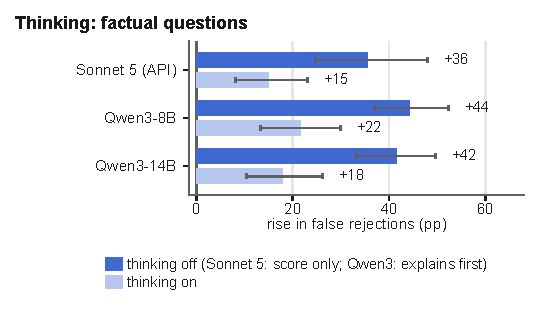
\includegraphics[width=0.66\textwidth]{figures/figA_thinking.pdf}
\caption{\textbf{On factual questions, thinking about halves the rise in false rejections.} Rise in false rejections on \textsc{MACE} without and with thinking: Sonnet~5 through the API (score only against adaptive thinking), Qwen3 judges (explanation first against thinking on). 95\% intervals.\pre}
\label{fig:thinking}
\end{figure}

\paragraph{Thinking on versus off.}
This pre-specified experiment reran the Qwen3-8B protocol of \cref{app:rotation} (rubric~$a$ ending in a ``Score: N'' line, temperature 0.6, top-p 0.95, top-k 20, up to 4,096 new tokens) with the chat template's thinking switch off and nothing else changed. The pools are the swap subsample and the 16-sample $k$-subsample of \cref{app:rotation}, plus a \textsc{MACE} subsample: every River or Language task with $k{>}1$ that has both matching and non-matching valid samples, with up to four samples each of matching-valid, non-matching-valid, and invalid answers (81 tasks, 825 samples). Twelve of 1,200 blind thinking-off replies on the $k$-subsample had no parseable score; none did elsewhere. \Cref{tab:toggle} gives the results. A second pre-specified toggle with Qwen3-14B repeats the pattern (\cref{tab:r4-toggle}). With thinking off, the loss under the swap is $-1.98$; with it on, $-0.12$. The \textsc{MACE} margin increase is $+7.07$ off and $+3.13$ on. With thinking on, Qwen3-14B's blind verification AUROC is 0.86 on the arithmetic subsample and 0.81 on the factual one (Qwen3-8B: 0.86 and 0.80).

\begin{table}[htbp]
\centering
\caption{Qwen3-8B with thinking off and on, same weights and prompt. Swap rows: change in score of identical valid text (points). Margin rows: referenced-minus-blind margin (points). False rejections: share of non-matching valid answers scored 3 or below, referenced minus blind (points). 95\% CI; mean generated tokens.\pre}
\label{tab:toggle}
\footnotesize
\setlength{\tabcolsep}{3pt}
\begin{adjustbox}{max width=\linewidth}\begin{tabular}{llccc}
\toprule
Task type & Readout & Thinking off & Thinking on & Tokens (off / on) \\
\midrule
Arithmetic (swap) & moved onto & $+0.567$ {\scriptsize$[+0.414,+0.747]$} & $-0.006$ {\scriptsize$[-0.017,+0.000]$} & 159 / 569 \\
 & moved off & $-0.694$ {\scriptsize$[-0.918,-0.471]$} & $+0.011$ {\scriptsize$[+0.000,+0.032]$} & \\
 & matches neither & $-0.035$ {\scriptsize$[-0.209,+0.142]$} & $-0.003$ {\scriptsize$[-0.009,+0.000]$} & \\
Arithmetic ($k$-subsample) & added margin & $+1.18$ {\scriptsize$[+0.25,+2.38]$} & $+0.06$ {\scriptsize$[-0.10,+0.26]$} & 193 / 1009 \\
Factual (MACE subsample) & added margin & $+6.16$ {\scriptsize$[+5.23,+7.15]$} & $+3.62$ {\scriptsize$[+2.55,+4.75]$} & 80 / 631 \\
 & false rejections, ref $-$ blind & $+44.3$ {\scriptsize$[+36.9,+52.3]$} & $+21.6$ {\scriptsize$[+13.3,+29.9]$} & \\
\bottomrule
\end{tabular}
\end{adjustbox}

\end{table}

With thinking on, valid swap samples receive 10 in 99.8\% of referenced replies and 96.2\% of blind ones; with thinking off, in 79.2\% and 76.9\%. The thinking judge's arithmetic scores therefore sit at the top of the scale whether or not the reference agrees, which leaves no room for a reference to raise them. A ceiling does not explain the missing loss, however: the same answers keep their scores when the reference moves off them ($+0.01$), although they were free to fall. On \textsc{MACE} its valid answers average 7.96 with the reference and 8.18 blind, away from the ceiling, and the anchoring returns. These diagnostics are post hoc.

\paragraph{Sonnet~5 with and without thinking.}
A pre-specified three-arm design tested the same contrast on a frontier judge through the Claude command-line tool, with the default system prompt replaced, no tools, and an empty working directory, on 60 replication-pool tasks with one sample each that gains, loses, or keeps neither reference under the swap. The score-only arm, with thinking off, anchors: $+3.57$ \ci{+2.57}{+4.55} for text the reference moves onto, $-2.85$ \ci{-3.85}{-1.92} for text it moves off, and $-0.07$ \ci{-1.18}{+1.10} for text matching neither, with 26.7\% \ci{20.4}{33.3} of correct non-matching answers scored 3 or below. Asking it to reason before a final ``Score: N'' line removes most of this, with thinking off ($+0.28$, $-0.20$ \ci{-0.37}{-0.05}, 0.4\% false rejections) or on ($+0.18$, $-0.32$ \ci{-0.67}{-0.07}, 0.4\%). All four registered predictions were confirmed; the reasoning and thinking arms were completed in a second session that re-ran only the calls that had failed.\pre{}
A second pre-specified experiment asked the same question on 40 factual \textsc{MACE} tasks, with one matching-correct, one non-matching-correct, and one wrong sample each, blind and referenced. The added margin is $+3.98$ \ci{+2.70}{+5.30} with a score only and $+3.03$ \ci{+1.70}{+4.65} with thinking on (paired difference $-0.95$ \ci{-2.45}{+0.63}), and the share of non-matching correct answers scored 3 or below rises by 17.5 and 12.5 points. Blind, Sonnet~5 ranks both correct answers above the wrong one 94.4\% and 96.9\% of the time, so it anchors on these questions although it can verify them; all three registered predictions were confirmed.\pre

\paragraph{Does acceptance mean verification, and does anchoring shrink where judges verify?}
Keeping answers a judge scored 7 or above without a reference is a weak test of verification for the open judges: that filter keeps 93\% of correct replication-pool answers for Qwen2.5-7B but also 24\% of wrong ones, and 96\% and 30\% for phi-4 (any-format labels). It is closer to verification for Sonnet~5, which scores 7 or above on 7\% to 16\% of wrong answers in its subsamples, and for GPT-4.1 (12\%). Across the 120 replication tasks, Qwen2.5-7B's swap size (the mean gain of text the reference moves onto and loss of text it moves off, exact scorer) falls as its blind AUROC rises (Spearman $-0.40$ \ci{-0.53}{-0.25}): it is 5.2 and 5.4 points in the lower two thirds of tasks (mean blind AUROC 0.83 and 0.93) and 3.6 points in the top third (0.98). Verification therefore reduces the effect but does not remove it where the judge already separates correct from wrong answers almost perfectly.\ph

\begin{table}[htbp]
\centering
\small
\caption{\textbf{Showing the reference raises the share of correct non-matching answers scored 3 or below, most on factual questions.} Points, referenced minus blind (95\% CI). Rows use different subsets and score readouts, so compare within a row; sources in \cref{tab:fr-sources}. Sonnet~5's two factual cells differ in design: the API cell uses 16-candidate subsamples (40 tasks), the command-line cells one answer per group (40 tasks).}
\label{tab:false-reject}
\setlength{\tabcolsep}{4pt}
\begin{adjustbox}{max width=\linewidth}\begin{tabular}{lcccc}
\toprule
 & \multicolumn{2}{c}{Arithmetic (constructed)} & \multicolumn{2}{c}{Factual (\textsc{MACE})} \\
\cmidrule(lr){2-3}\cmidrule(lr){4-5}
Judge & Thinking off & Thinking on & Thinking off & Thinking on \\
\midrule
Qwen2.5-7B & $+27.7$ {\scriptsize$[+22.8,+33.2]$}\pre & n/a & $+63.8$ {\scriptsize$[+56.6,+70.2]$}\ph & n/a \\
phi-4 & $+5.8$ {\scriptsize$[+2.9,+8.6]$}\ph & n/a & $+54.4$ {\scriptsize$[+46.9,+61.4]$}\ph & n/a \\
Qwen3-8B & $+1.5$ {\scriptsize$[+0.5,+2.6]$}\ph & $+0.0$ {\scriptsize$[+0.0,+0.0]$}\ph & $+44.3$ {\scriptsize$[+36.9,+52.3]$}\pre & $+21.6$ {\scriptsize$[+13.3,+29.9]$}\pre \\
Qwen3-14B & $+6.1$ {\scriptsize$[+3.8,+8.5]$}\ph & $+0.3$ {\scriptsize$[+0.0,+0.7]$}\ph & $+41.6$ {\scriptsize$[+33.2,+49.6]$}\pre & $+17.8$ {\scriptsize$[+10.4,+26.2]$}\pre \\
Sonnet~5, API & $+9.2$ {\scriptsize$[+5.1,+14.6]$}\pre & not run & $+35.6$ {\scriptsize$[+24.8,+48.0]$}\pre & not run \\
Sonnet~5, CLI & not run & not run & $+17.5$ {\scriptsize$[+5.0,+30.0]$}\pre & $+12.5$ {\scriptsize$[+2.5,+25.0]$}\pre \\
\bottomrule
\end{tabular}
\end{adjustbox}
\end{table}

\paragraph{End to end on \textsc{MACE}.}
The last pre-specified experiment measured selection accuracy on the benchmark's natural mix of $k$: all 133 River and Language tasks in the pass-rate band (34 with $k{=}1$, 99 with $k{>}1$), best of 64, rubric-$a$ selection. Blind and referenced scores are the frozen files of \cref{app:mace}, whose blind scores correlate with validity at $0.361$ (Qwen2.5-7B) and $0.477$ (phi-4); blind-then-reveal and the validity gate were run new with the prompts of \cref{app:setup}. We predicted that the reference would lower accuracy at $k{>}1$, that blind-then-reveal would beat it there, and that blind-then-reveal would be at least as accurate over the natural mix. All three predictions failed for both judges (\cref{tab:mace-accuracy}). The anchoring on these questions is large (\cref{app:mace}), but blind judges that verify factual answers this poorly gain more from the reference's help against wrong answers than they lose to its pull away from correct ones.

\begin{table}[htbp]
\centering
\caption{\textsc{MACE} River and Language: best-of-64 selection accuracy (\%) by protocol, and differences in points (95\% CI).\pre}
\label{tab:mace-accuracy}
\footnotesize
\setlength{\tabcolsep}{3pt}
\begin{adjustbox}{max width=\linewidth}\begin{tabular}{llcccccc}
\toprule
Judge & Tasks & Blind & Reference & Blind, then reveal & Validity gate & Reference $-$ blind & Reveal $-$ reference \\
\midrule
Qwen2.5-7B & $k{=}1$ (34) & 67.7 & 100.0 & 91.2 & 91.2 & $+32.4$ {\scriptsize$[+17.6,+47.1]$} & $-8.8$ {\scriptsize$[-20.6,+0.0]$} \\
 & $k{>}1$ (99) & 86.9 & 88.9 & 87.9 & 91.9 & $+2.0$ {\scriptsize$[-5.1,+9.1]$} & $-1.0$ {\scriptsize$[-7.1,+6.1]$} \\
 & all (133) & 82.0 & 91.7 & 88.7 & 91.7 & $+9.8$ {\scriptsize$[+2.3,+17.3]$} & $-3.0$ {\scriptsize$[-8.3,+2.3]$} \\
\addlinespace
phi-4 & $k{=}1$ (34) & 73.5 & 100.0 & 100.0 & 82.3 & $+26.5$ {\scriptsize$[+11.8,+41.2]$} & $+0.0$ {\scriptsize$[+0.0,+0.0]$} \\
 & $k{>}1$ (99) & 87.9 & 93.9 & 91.9 & 90.9 & $+6.1$ {\scriptsize$[-1.0,+13.1]$} & $-2.0$ {\scriptsize$[-6.1,+2.0]$} \\
 & all (133) & 84.2 & 95.5 & 94.0 & 88.7 & $+11.3$ {\scriptsize$[+5.2,+18.1]$} & $-1.5$ {\scriptsize$[-4.5,+1.5]$} \\
\bottomrule
\end{tabular}
\end{adjustbox}

\end{table}

%==========================================================================================
\FloatBarrier
\section{Swap test: all cells and the judge-size ladder}
\label{app:rotation}

The ledger calls the swap test \emph{rot\-ation}: the reference is moved to a different correct answer while the candidate text stays fixed.

The swap assigns each task the valid alternative that appears most often among its valid samples, so that enough samples match the new reference. This choice makes cross-sample margins partly reflect how common an answer is; the paired same-sample changes in \cref{tab:rotation} compare each sample with itself and are not affected.

\begin{table}[htbp]
\centering
\caption{Change in score of identical text when the reference is swapped (replication pool, 0--10 scale, 95\% CI; original scorer, registered runs; exact-scorer values for Qwen2.5-7B are in \cref{tab:r4-rotation}).\pre{} ``Onto'': samples that match the new reference. ``Off'': samples that matched only the old one. ``Neither'': valid samples matching neither. The last row keeps only samples Sonnet~5 scored at least 7 blind (3,194 of 3,494). For the open judges the analogous filter on each judge's own blind score gives $+4.99$ \ci{+4.69}{+5.32} (Qwen2.5-7B, 91\% kept) and $+4.08$ (phi-4, 98\% kept).\ph}
\label{tab:rotation}
\footnotesize
\setlength{\tabcolsep}{3pt}
\begin{adjustbox}{max width=\linewidth}\begin{tabular}{llcccc}
\toprule
Judge & Rubric & Moved onto ($n{=}120$) & Moved off ($n{=}93$) & Neither ($n{=}113$) & Onto minus neither \\
\midrule
Qwen2.5-7B & $a$ & $+4.97$ {\scriptsize$[+4.66,+5.27]$} & $-5.04$ {\scriptsize$[-5.38,-4.67]$} & $+0.13$ {\scriptsize$[-0.04,+0.31]$} & $+4.81$ {\scriptsize$[+4.44,+5.17]$} \\
 & $b$ & $+6.34$ {\scriptsize$[+6.10,+6.60]$} & $-6.58$ {\scriptsize$[-6.89,-6.26]$} & $+0.10$ {\scriptsize$[-0.11,+0.29]$} & $+6.18$ {\scriptsize$[+5.84,+6.50]$} \\
phi-4 & $a$ & $+4.09$ {\scriptsize$[+3.79,+4.38]$} & $-3.92$ {\scriptsize$[-4.26,-3.59]$} & $+0.30$ {\scriptsize$[+0.04,+0.57]$} & $+3.88$ {\scriptsize$[+3.52,+4.25]$} \\
 & $b$ & $+3.25$ {\scriptsize$[+2.95,+3.51]$} & $-3.18$ {\scriptsize$[-3.46,-2.87]$} & $+0.24$ {\scriptsize$[+0.01,+0.47]$} & $+3.08$ {\scriptsize$[+2.76,+3.41]$} \\
Claude Sonnet 5 & $a$ & $+3.04$ {\scriptsize$[+2.53,+3.56]$} & $-2.66$ {\scriptsize$[-3.36,-2.00]$} & $+0.04$ {\scriptsize$[-0.41,+0.46]$} & $+3.08$ {\scriptsize$[+2.45,+3.78]$} \\
 & $b$ & $+2.54$ {\scriptsize$[+2.04,+3.08]$} & $-2.51$ {\scriptsize$[-3.17,-1.89]$} & $+0.28$ {\scriptsize$[-0.10,+0.69]$} & $+2.31$ {\scriptsize$[+1.75,+2.86]$} \\
\quad blind-accepted only & $a$ & $+2.79$ {\scriptsize$[+2.26,+3.40]$} & $-2.50$ {\scriptsize$[-3.20,-1.83]$} & $+0.20$ {\scriptsize$[-0.21,+0.65]$} & $+2.67$ {\scriptsize$[+2.04,+3.33]$} \\
\bottomrule
\end{tabular}
\end{adjustbox}

\end{table}

Before the replication, we ran the same test on the exploratory Ties pool at four Qwen2.5 judge sizes (\cref{tab:ladder}). The effect is largest for small judges, where it saturates the scale, and smaller but present at 14B. On the same split, blind margins are small, and samples matching neither reference move between $-0.44$ and $+0.82$. Restricting to samples the 7B judge scored at least 7 blind gives $+4.74$ \ci{+3.67}{+5.87} against $+4.57$ unfiltered.

\begin{table}[htbp]
\centering
\caption{Swap on the exploratory Ties pool, Qwen2.5 judges (0--10 scale).\pre}
\label{tab:ladder}
\footnotesize
\setlength{\tabcolsep}{4pt}
\begin{tabular}{llcccc}
\toprule
Readout & Rubric & 1.5B & 3B & 7B & 14B \\
\midrule
Gain, reference moved onto the sample ($n{=}40$) & $a$ & $+9.48$ & $+9.29$ & $+4.57$ & $+3.07$ \\
 & $b$ & $+8.73$ & $+9.58$ & $+5.96$ & $+3.47$ \\
Loss, reference moved off the sample ($n{=}10$) & $a$ & $-9.65$ & $-8.85$ & $-3.14$ & $-2.78$ \\
 & $b$ & $-9.42$ & $-9.80$ & $-4.71$ & $-3.81$ \\
Referenced margin ($n{=}18$) & $a$ & $+9.00$ & $+9.05$ & $+4.75$ & $+3.26$ \\
 & $b$ & $+8.36$ & $+9.12$ & $+5.93$ & $+3.67$ \\
Blind margin, same split ($n{=}18$) & $a$ & $+0.16$ & $+1.36$ & $+0.31$ & $+0.69$ \\
 & $b$ & $+0.61$ & $+1.91$ & $+0.14$ & $+0.04$ \\
\bottomrule
\end{tabular}

\end{table}

\paragraph{Judges that explain or think before scoring.}
A later pre-specified experiment re-ran the swap on a subsample of the replication pool (up to three samples per class per task, 879 samples) and the $k$ comparison on a 16-sample subsample of the $k$-pool, under two protocols: the verbatim MT-Bench single-answer templates with Qwen2.5-7B (the reference version asks the judge to begin ``by comparing the assistant's answer with the reference answer'' and to explain before a rating from 1 to 10), and Qwen3-8B with thinking enabled (temperature 0.6, up to 4,096 new tokens, rubric~$a$ ending in a ``Score: N'' line). Replies without a parseable score were dropped (20 of 879 swap pairs for MT-Bench; none for the thinking judge's swap replies). \Cref{tab:r2b} gives the results; accuracy is best-of-16.

\begin{table}[htbp]
\centering
\caption{Judges that write before scoring: change in score of identical text under the swap (points, 95\% CI).\pre}
\label{tab:r2b}
\footnotesize
\setlength{\tabcolsep}{3pt}
\begin{adjustbox}{max width=\linewidth}\begin{tabular}{lccc}
\toprule
Protocol & Moved onto & No longer matches & Neither \\
\midrule
MT-Bench template, Qwen2.5-7B & $+3.618$ {\scriptsize$[+3.401,+3.842]$} & $-3.591$ {\scriptsize$[-3.936,-3.242]$} & $+0.077$ {\scriptsize$[-0.212,+0.404]$} \\
Thinking judge, Qwen3-8B & $-0.006$ {\scriptsize$[-0.017,+0.000]$} & $+0.011$ {\scriptsize$[+0.000,+0.032]$} & $-0.003$ {\scriptsize$[-0.009,+0.000]$} \\
\bottomrule
\end{tabular}
\end{adjustbox}

\end{table}

\begin{table}[htbp]
\centering
\caption{Judges that write before scoring on the 16-sample $k$-subsample: referenced-minus-blind margin at $k{>}1$ (points) and change in best-of-16 selection accuracy (points, 95\% CI).\pre}
\label{tab:r2b-k}
\footnotesize
\begin{adjustbox}{max width=\linewidth}\begin{tabular}{lccc}
\toprule
Protocol & Margin, $k{>}1$ (ref $-$ blind) & Accuracy change, $k{=}1$ & Accuracy change, $k{>}1$ \\
\midrule
MT-Bench template, Qwen2.5-7B & $+3.19$ {\scriptsize$[+2.57,+3.88]$} & $+16.6$ {\scriptsize$[-1.5,+34.2]$} & $-13.0$ {\scriptsize$[-25.1,-1.1]$} \\
Thinking judge, Qwen3-8B & $+0.06$ {\scriptsize$[-0.10,+0.26]$} & $-5.8$ {\scriptsize$[-11.4,-1.8]$} & $-3.7$ {\scriptsize$[-7.5,+0.0]$} \\
\bottomrule
\end{tabular}
\end{adjustbox}

\end{table}
The thinking judge gives a score of 10 to 96.2\% of valid swap samples blind and to 99.8\% with either reference, while invalid $k$-subsample answers average 3.67 blind and 3.15 with the reference; it writes 569 to 1,092 tokens on average, and 82.7\% of its referenced swap replies mention the reference in their final text. Under the MT-Bench template, by contrast, the mean score of valid swap samples falls from 6.68 blind to 4.97 with the reference, and its explanations average 259 tokens. These diagnostics are post hoc.

%==========================================================================================
\FloatBarrier
\section{Mechanism details}
\label{app:mechanism}

\begin{table}[htbp]
\centering
\caption{Masking suite: margin by how the reference is written (0--10 scale, 95\% CI). Numeral, words, and expression use 93 replication-pool tasks; the worked-solution columns use 21 $k$-pool tasks with a single-number answer.\pre}
\label{tab:masking}
\footnotesize
\setlength{\tabcolsep}{3pt}
\begin{adjustbox}{max width=\linewidth}\begin{tabular}{llcccc}
\toprule
Judge & Rubric & Numeral & Words & Expression & Worked: visible $\to$ masked \\
\midrule
Qwen2.5-7B & $a$ & $+4.62$ {\scriptsize$[+4.32,+4.96]$} & $+2.88$ {\scriptsize$[+2.47,+3.28]$} & $+0.29$ {\scriptsize$[+0.07,+0.49]$} & $+2.97$ {\scriptsize$[+2.01,+4.06]$} $\to$ $+0.05$ {\scriptsize$[-0.52,+0.63]$} \\
 & $b$ & $+5.99$ {\scriptsize$[+5.69,+6.29]$} & $+4.60$ {\scriptsize$[+4.14,+5.03]$} & $+0.35$ {\scriptsize$[+0.12,+0.56]$} & $+4.62$ {\scriptsize$[+3.57,+5.78]$} $\to$ $+0.31$ {\scriptsize$[-0.46,+1.13]$} \\
phi-4 & $a$ & $+3.79$ {\scriptsize$[+3.48,+4.11]$} & $+3.68$ {\scriptsize$[+3.27,+4.06]$} & $+0.89$ {\scriptsize$[+0.64,+1.13]$} & $+3.51$ {\scriptsize$[+3.06,+4.01]$} $\to$ $-0.49$ {\scriptsize$[-1.27,+0.26]$} \\
 & $b$ & $+3.11$ {\scriptsize$[+2.83,+3.39]$} & $+3.01$ {\scriptsize$[+2.71,+3.37]$} & $+0.63$ {\scriptsize$[+0.45,+0.82]$} & $+2.84$ {\scriptsize$[+2.40,+3.28]$} $\to$ $-0.45$ {\scriptsize$[-1.11,+0.12]$} \\
\bottomrule
\end{tabular}
\end{adjustbox}

\end{table}

\paragraph{Decode cost.}
We kept the answer an integer and re-encoded the reference with one, two, or three reversible steps (a digit shift; then base64; then string reversal), stating the decoding rule each time. We had predicted a graded decline. For Qwen2.5-7B the margin instead collapsed at the first step and stayed at zero (\cref{tab:cipher}). Every encoded prompt announced that the reference had been encoded, and that framing may explain the collapse by itself: ``30+1'', a comparable single step without such framing, cut the margin by 94\% and 77\% but did not remove it. The phi-4 cells are not evaluable. A later audit found that 81.0\% to 97.6\% of phi-4's encoded-reference replies contained no score, so the scorer substituted 5.0, and its near-zero margins measure that substitution rather than the judge. All of Qwen2.5-7B's replies contained scores.

\begin{table}[htbp]
\centering
\caption{Margin with the reference encoded by one to three stated decoding steps (0--10 scale, 95\% CI, 93 tasks). The phi-4 decoding cells are not evaluable: most of its replies contained no score and were set to 5.0 by the scorer.\pre}
\label{tab:cipher}
\footnotesize
\begin{adjustbox}{max width=\linewidth}\begin{tabular}{lcccc}
\toprule
Judge & Plain reference & One decode step & Two steps & Three steps \\
\midrule
Qwen2.5-7B & $+4.62$ {\scriptsize$[+4.32,+4.96]$} & $-0.18$ {\scriptsize$[-0.44,+0.08]$} & $-0.28$ {\scriptsize$[-0.57,+0.00]$} & $-0.27$ {\scriptsize$[-0.56,+0.00]$} \\
phi-4 & $+3.79$ {\scriptsize$[+3.46,+4.12]$} & $-0.02$ {\scriptsize$[-0.07,+0.03]$} & $+0.00$ {\scriptsize$[+0.00,+0.01]$} & $+0.01$ {\scriptsize$[+0.00,+0.01]$} \\
\bottomrule
\end{tabular}
\end{adjustbox}

\end{table}

\paragraph{Solution route.}
Holding the reference answer fixed and swapping its derivation to a different method moves the identical sample's score by $-0.32$ and $-0.40$ points for Qwen2.5-7B and $-0.02$ for phi-4. The registered no-change prediction fails for Qwen2.5-7B, whose interval excludes zero, and holds for phi-4, whose interval reaches zero; the effects are 20 to 400 times smaller than swapping the answer, and a preference for samples whose own route matches the shown one appears in one of four cells.

%==========================================================================================
\FloatBarrier
\section{Frontier judges}
\label{app:frontier}

\paragraph{An excluded command-line check.}
An earlier check called \texttt{claude -p --model sonnet} from the project directory in August 2026 on 37 $k$-pool tasks. It ran with the interface's default agent context, which may have shown repository metadata naming the hypothesis, and with extended thinking on 178 of 330 blind but 27 of 330 referenced calls, so we exclude it from the ledger counts and the main text. For the record, its mean per-task margin was $+0.35$ \ci{-0.56}{+1.27} blind and $+7.49$ \ci{+6.58}{+8.27} with the reference, and it scored 19.6\% of correct non-matching answers at 3 or below blind and 82.5\% with the reference, pooled over samples. The command-line replication of \cref{app:reasoning} removes this context.

\paragraph{API judges.}
Sonnet~5 reproduces the swap (\cref{tab:rotation}), the blind-accepted filter, the masking pattern (bare reference $+3.06$, words $+3.14$, expression $+0.47$), and the \textsc{MACE} result that its blind margin is negative. GPT-4.1 picks matching answers far more often with the reference (32 referenced-only against 1 blind-only picks) and has a margin of $+1.19$. It failed our pre-specified score-resolution screen: an average of 15.03 candidates per pool tie at its maximum score, against a bar of 3.0. Its $k$ step is $+0.27$ \ci{-0.02}{+0.61} on the $k$-pool and $-0.08$ \ci{-0.49}{+0.20} on the synthetic grid, where ties are heavier (47.0 per pool), so we report it as unresolved.

\begin{table}[htbp]
\centering
\caption{API judges (inflation in \sd, margins in points, 95\% CI). GPT-4.1's inflation and step rows are unreliable because of ties. Sonnet~5's inflation and step were not run: its tool-call scores are integers and tie under best-of-64.\pre}
\label{tab:frontier-api}
\footnotesize
\begin{adjustbox}{max width=\linewidth}\begin{tabular}{lcc}
\toprule
Readout & GPT-4.1 & Claude Sonnet 5 \\
\midrule
Replication pool: added inflation ($n{=}105$) & $+0.12$ {\scriptsize$[+0.02,+0.23]$} & --- \\
Replication pool: referenced-only / blind-only picks & 32 / 1 & --- \\
Replication pool: margin & $+1.19$ {\scriptsize$[+0.92,+1.50]$} & --- \\
$k$-pool: step $k{>}1$ minus $k{=}1$ & $+0.27$ {\scriptsize$[-0.02,+0.61]$} & --- \\
$k$-pool margin, reference & $+0.99$ {\scriptsize$[+0.57,+1.55]$} & $+3.00$ {\scriptsize$[+2.02,+4.02]$} \\
\quad + any-valid-answer instruction & $+0.46$ {\scriptsize$[+0.13,+0.94]$} & $+2.08$ {\scriptsize$[+1.14,+3.14]$} \\
\quad + do-not-compare instruction & $+0.59$ {\scriptsize$[+0.21,+1.12]$} & $+2.60$ {\scriptsize$[+1.59,+3.66]$} \\
$k$-pool margin, blind & $+0.09$ {\scriptsize$[-0.46,+0.74]$} & $+0.20$ {\scriptsize$[-0.46,+0.99]$} \\
\bottomrule
\end{tabular}
\end{adjustbox}

\end{table}

\paragraph{Sonnet~5 with wrong answers.}
The first Sonnet~5 API scores (\cref{tab:round7}) covered correct answers only. A pre-specified experiment scored 16-candidate subsamples that include wrong answers, blind and with the reference: 40 replication tasks (8 per family), 40 \textsc{MACE} tasks with $k{>}1$, and all 22 eligible $k$-pool tasks with $k{>}1$, each subsample holding at least one matching-correct, one non-matching-correct, and one wrong answer. It began through the command-line interface and stopped at the account's spend limit after 939 of the 1,280 replication calls; a registered amendment re-ran every call through the Messages API with extended thinking disabled and the same prompts, and those scores give the results (\cref{tab:sonnet-r8}).\pre{} Before the amendment we had seen the partial command-line readouts on 24 replication tasks, which the amendment records. On the 939 calls that both interfaces completed, command-line and API scores agree exactly on 67\% and within one point on 82\%, and API scores are 0.38 points higher on average, so we do not compare command-line and API results for Sonnet~5 directly.\ph

\begin{table}[htbp]
\centering
\caption{Sonnet~5 (Messages API, thinking disabled) on 16-candidate subsamples with wrong answers: referenced minus blind unless stated (95\% CI). Replication and $k$-pool use answers read in any format; ``registered'' uses the registered checker.\pre}
\label{tab:sonnet-r8}
\footnotesize
\setlength{\tabcolsep}{3pt}
\begin{adjustbox}{max width=\linewidth}\begin{tabular}{lcccc}
\toprule
Readout & Replication & Repl., registered & \textsc{MACE}, $k{>}1$ & $k$-pool, $k{>}1$ \\
\midrule
Tasks with all 32 calls scored & 40 & 40 & 40 & 22 \\
AUROC, non-matching vs.\ wrong: blind & 0.96 {\scriptsize$[0.94,0.98]$} & 0.92 {\scriptsize$[0.89,0.94]$} & 0.94 {\scriptsize$[0.91,0.97]$} & 0.94 {\scriptsize$[0.91,0.97]$} \\
\quad with the reference & 0.92 {\scriptsize$[0.89,0.95]$} & 0.86 {\scriptsize$[0.82,0.90]$} & 0.78 {\scriptsize$[0.71,0.85]$} & 0.86 {\scriptsize$[0.81,0.91]$} \\
\quad change & $-0.04$ {\scriptsize$[-0.07,-0.01]$} & $-0.05$ {\scriptsize$[-0.08,-0.02]$} & $-0.15$ {\scriptsize$[-0.22,-0.10]$} & $-0.08$ {\scriptsize$[-0.12,-0.04]$} \\
AUROC, all correct vs.\ wrong: change & $-0.03$ {\scriptsize$[-0.05,+0.00]$} & $-0.04$ {\scriptsize$[-0.06,-0.01]$} & $-0.08$ {\scriptsize$[-0.12,-0.04]$} & $-0.05$ {\scriptsize$[-0.08,-0.02]$} \\
False rejections, change (points) & $+9.2$ {\scriptsize$[+5.1,+14.6]$} & $+8.7$ {\scriptsize$[+4.3,+14.1]$} & $+35.6$ {\scriptsize$[+24.8,+48.0]$} & $+22.5$ {\scriptsize$[+11.8,+35.1]$} \\
Margin, change (points of 10) & $+1.58$ {\scriptsize$[+1.07,+2.16]$} & $+1.58$ {\scriptsize$[+0.90,+2.25]$} & $+4.21$ {\scriptsize$[+2.89,+5.65]$} & $+2.57$ {\scriptsize$[+1.75,+3.50]$} \\
Best-of-16 accuracy, change (points) & $+1.3$ {\scriptsize$[-1.6,+4.2]$} & $-1.1$ {\scriptsize$[-6.5,+4.0]$} & $+1.4$ {\scriptsize$[-1.3,+4.7]$} & $-2.6$ {\scriptsize$[-5.8,+0.4]$} \\
Max rule accuracy, change (points) & $+0.0$ {\scriptsize$[-1.9,+2.3]$} & $-2.0$ {\scriptsize$[-6.5,+2.1]$} & $+0.2$ {\scriptsize$[-1.8,+2.7]$} & $-2.4$ {\scriptsize$[-5.0,-0.5]$} \\
\bottomrule
\end{tabular}
\end{adjustbox}
\end{table}

\begin{table}[htbp]
\centering
\caption{Sources of the cells of \cref{tab:false-reject}: value (points, 95\% CI), pool, scorer or experiment, and number of tasks.}
\label{tab:fr-sources}
\footnotesize
\begin{adjustbox}{max width=\linewidth}\begin{tabular}{llL{6.2cm}}
\toprule
Judge & Cell & Value (95\% CI), source \\
\midrule
Qwen2.5-7B & arithmetic, thinking off & $+27.7$ {\scriptsize$[+22.8,+33.2]$}; replication, exact scorer (93 tasks) \\
Qwen2.5-7B & factual, thinking off & $+63.8$ {\scriptsize$[+56.6,+70.2]$}; \textsc{MACE} $k{>}1$, exact scorer (91 tasks) \\
phi-4 & arithmetic, thinking off & $+5.8$ {\scriptsize$[+2.9,+8.6]$}; replication (93 tasks) \\
phi-4 & factual, thinking off & $+54.4$ {\scriptsize$[+46.9,+61.4]$}; \textsc{MACE} $k{>}1$ (91 tasks) \\
Qwen3-8B & arithmetic, thinking off & $+1.5$ {\scriptsize$[+0.5,+2.6]$}; swap subsample (120 tasks) \\
Qwen3-8B & arithmetic, thinking on & $+0.0$ {\scriptsize$[+0.0,+0.0]$}; swap subsample (120 tasks) \\
Qwen3-8B & factual, thinking off & $+44.3$ {\scriptsize$[+36.9,+52.3]$}; MACE subsample, thinking toggle (81 tasks) \\
Qwen3-8B & factual, thinking on & $+21.6$ {\scriptsize$[+13.3,+29.9]$}; MACE subsample, thinking toggle (81 tasks) \\
Qwen3-14B & arithmetic, thinking off & $+6.1$ {\scriptsize$[+3.8,+8.5]$}; swap subsample (120 tasks) \\
Qwen3-14B & arithmetic, thinking on & $+0.3$ {\scriptsize$[+0.0,+0.7]$}; swap subsample (120 tasks) \\
Qwen3-14B & factual, thinking off & $+41.6$ {\scriptsize$[+33.2,+49.6]$}; MACE subsample, thinking toggle (81 tasks) \\
Qwen3-14B & factual, thinking on & $+17.8$ {\scriptsize$[+10.4,+26.2]$}; MACE subsample, thinking toggle (81 tasks) \\
Sonnet~5, API & arithmetic, thinking off & $+9.2$ {\scriptsize$[+5.1,+14.6]$}; replication subsamples with wrong answers, any-format labels, API (40 tasks) \\
Sonnet~5, API & factual, thinking off & $+35.6$ {\scriptsize$[+24.8,+48.0]$}; MACE subsamples with wrong answers, API (40 tasks) \\
Sonnet~5, CLI & factual, thinking off & $+17.5$ {\scriptsize$[+5.0,+30.0]$}; MACE, one answer of each kind, CLI (40 tasks) \\
Sonnet~5, CLI & factual, thinking on & $+12.5$ {\scriptsize$[+2.5,+25.0]$}; MACE, one answer of each kind, CLI (40 tasks) \\
\bottomrule
\end{tabular}
\end{adjustbox}
\end{table}

%==========================================================================================
\FloatBarrier
\section{Acceptance, the full-credit sentence, and benchmark scores}
\label{app:acceptance}

\begin{figure}[htbp]
\centering
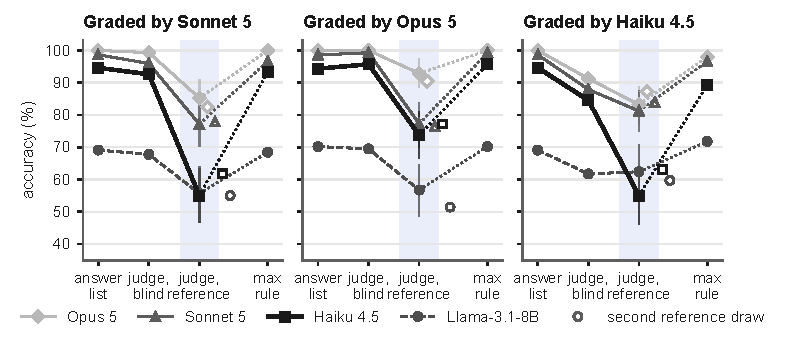
\includegraphics[width=\textwidth]{figures/fig4_benchmark.pdf}
\caption{\textbf{Shown the reference, every grader scores the models below their answer lists; blind, Sonnet~5 and Opus~5 stay within 3 points of them.} One answer per model on 149 \textsc{MACE} questions with several correct answers, scored by the answer lists and by each judge, blind, with the reference, and under the max rule (dotted); a score of 7 or above counts as correct; vertical lines are 95\% intervals for referenced accuracy; hollow markers use a second reference drawn from each answer list. Opus~5's panel uses 141 questions (136 for hollow markers) because its reasoning ran past the token limit on some referenced calls, which may understate its shortfall. Pre-specified, except Sonnet~5's max rule.}
\label{fig:benchmark}
\end{figure}

\paragraph{Opus~5 on the Sonnet~5 subsamples.}
A pre-specified experiment ran Claude Opus~5 (\texttt{claude-opus-5}) through the Messages API with thinking disabled, with the prompts and 16-candidate subsamples of \cref{app:frontier}: 3,264 calls, no errors, and 10 replies without a score, treated as missing (9 on \textsc{MACE}, cut off at 512 tokens). Grading AUROC for correct non-matching answers changes by $-0.164$ \ci{-0.223}{-0.110} on \textsc{MACE}, $-0.057$ \ci{-0.117}{-0.013} on the $k$-pool, and $-0.015$ \ci{-0.038}{+0.009} on the replication pool, and false rejections on \textsc{MACE} rise by 36.3 points \ci{+26.7}{+46.7}. Pooled over the three pools, 76 of 525 non-matching correct answers scored 10 blind fall to 3 or below with the reference, against 0 of 247 matching ones. We predicted that at most 5\% of wrong answers would score 10 blind in each pool; 5.9\%, 5.1\%, and 8.2\% did (replication, \textsc{MACE}, $k$-pool), so a blind 10 is a slightly weaker sign of verification for Opus~5 than for Sonnet~5 (1.8\% to 3.7\%). Although thinking was disabled and the rubric asks for a score only, Opus~5 wrote visible reasoning before its score on 24\% to 33\% of blind calls and 12\% to 16\% of referenced calls. We parsed the last integer, which was the final score in every reply we inspected; restricting to answers whose two calls both gave a bare score leaves the \textsc{MACE} false-rejection rise essentially unchanged ($+35.3$ against $+35.0$ points).\ph

\paragraph{Sonnet~5 with thinking through the API.}
A pre-specified experiment re-ran the 40 \textsc{MACE} subsamples with adaptive thinking (1,280 calls, none failed or unparseable). Grading AUROC changes by $-0.091$ \ci{-0.140}{-0.050}, against $-0.153$ with thinking disabled, and false rejections rise by 14.9 points \ci{+8.2}{+23.1}, against 35.6; all three predictions were confirmed. With thinking, Sonnet~5 gives a blind 10 to none of 258 wrong answers but also to only 22 of 382 correct ones, too few to test acceptance: 1 of the 13 non-matching answers it scored 10 blind falls to 3 or below with the reference, against 0 of 9 matching ones.

\paragraph{A second blind call.}
A pre-specified experiment re-scored blind, through the same interface and with the same settings, every correct answer that each API judge had scored 10 on its first blind call (\cref{tab:r20-retest}). On the second call Sonnet~5 gives 3 or below to none of the 318 non-matching answers and still gives 10 to 87.1\% of them; Opus~5 gives 3 or below to 2 of 525 and 10 to 96.2\%. All three predictions were confirmed. One of Opus~5's second calls, on a matching \textsc{MACE} answer, returned no score. An earlier noise floor re-scored replication answers through the command-line interface and compared two interfaces; this experiment supersedes it.

\begin{table}[htbp]
\centering
\caption{Correct answers each API judge scored 10 on its first blind call: how many score 3 or below with the reference, and on a second blind call through the same interface. One of Opus~5's second calls, on a matching \textsc{MACE} answer, returned no score, so its pooled matching count is 246 here and 247 in the registered acceptance readout.\pre}
\label{tab:r20-retest}
\footnotesize
\begin{adjustbox}{max width=\linewidth}\begin{tabular}{llrrrrrr}
\toprule
 & & \multicolumn{3}{c}{Differ from the reference} & \multicolumn{3}{c}{Match the reference} \\
\cmidrule(lr){3-5}\cmidrule(lr){6-8}
Judge & Pool & Blind 10 & Ref.\ $\leq 3$ & Retest $\leq 3$ & Blind 10 & Ref.\ $\leq 3$ & Retest $\leq 3$ \\
\midrule
Sonnet 5 & \textsc{MACE}, $k{>}1$ & 81 & 15 (18.5\%) & 0 (0.0\%) & 38 & 0 (0.0\%) & 0 (0.0\%) \\
 & Replication & 150 & 13 (8.7\%) & 0 (0.0\%) & 60 & 0 (0.0\%) & 0 (0.0\%) \\
 & $k$-pool, $k{>}1$ & 87 & 13 (14.9\%) & 0 (0.0\%) & 39 & 0 (0.0\%) & 0 (0.0\%) \\
 & Pooled & 318 & 41 (12.9\%) & 0 (0.0\%) & 137 & 0 (0.0\%) & 0 (0.0\%) \\
\addlinespace
Opus 5 & \textsc{MACE}, $k{>}1$ & 201 & 63 (31.3\%) & 2 (1.0\%) & 102 & 0 (0.0\%) & 0 (0.0\%) \\
 & Replication & 211 & 10 (4.7\%) & 0 (0.0\%) & 88 & 0 (0.0\%) & 0 (0.0\%) \\
 & $k$-pool, $k{>}1$ & 113 & 3 (2.7\%) & 0 (0.0\%) & 56 & 0 (0.0\%) & 0 (0.0\%) \\
 & Pooled & 525 & 76 (14.5\%) & 2 (0.4\%) & 246 & 0 (0.0\%) & 0 (0.0\%) \\
\addlinespace
Both judges & Pooled & 843 & 117 (13.9\%) & 2 (0.2\%) & 383 & 0 (0.0\%) & 0 (0.0\%) \\
Both judges & \textsc{MACE}, $k{>}1$ & 282 & 78 (27.7\%) & 2 (0.7\%) & 140 & 0 (0.0\%) & 0 (0.0\%) \\
\bottomrule
\end{tabular}
\end{adjustbox}
\end{table}

\paragraph{A matched acceptance threshold for the open judges.}
Open judges' expected scores are deterministic, so a second call would repeat the first, and they rarely give any answer exactly 10. For each open judge and pool we took the lowest blind expected score, on a grid of 0.05, that at most 3\% of wrong answers reach, and asked how often correct answers at or above it score 3 or below with the reference (\cref{tab:r20-matched}). On the constructed pools, 5\% to 57\% of those that differ from the reference score 3 or below, against at most 0.4\% of those that match; on \textsc{MACE}, 83.3\% (Qwen2.5-7B) and 41.9\% (phi-4), against none of the matching ones, and a 5\% threshold gives 85.0\% and 43.0\%.\ph{} For Qwen3 on the 81-task \textsc{MACE} subsample we use a blind 10, which with thinking on 21\% to 24\% of wrong answers also receive, so those rows do not isolate acceptance; we report them for completeness.

\begin{table}[htbp]
\centering
\caption{Acceptance at a matched threshold for the open judges (full 64-candidate pools; any-format labels on the constructed pools, answer lists on \textsc{MACE}; exact scorer for Qwen2.5 and gemma-2), and at a blind 10 for Qwen3 on the \textsc{MACE} subsample. Threshold: the lowest blind expected score that at most 3\% of wrong answers reach.\ph}
\label{tab:r20-matched}
\footnotesize
\setlength{\tabcolsep}{2.6pt}
\begin{tabular}{llrrrr}
\toprule
 & & & & \multicolumn{2}{c}{Accepted: $n$; share $\leq 3$ with ref.} \\
\cmidrule(lr){5-6}
Judge & Pool & Threshold & Wrong accepted & Differ & Match \\
\midrule
Qwen2.5-7B & Replication & 9.80 & 3.0\% of 3491 & 1747; 19.2\% & 466; 0.4\% \\
phi-4 & Replication & 9.75 & 2.6\% of 3491 & 1839; 4.6\% & 530; 0.0\% \\
Qwen2.5-7B & $k$-pool, $k{>}1$ & 9.85 & 2.7\% of 2012 & 699; 25.0\% & 193; 0.0\% \\
phi-4 & $k$-pool, $k{>}1$ & 9.70 & 2.9\% of 2012 & 714; 15.4\% & 230; 0.0\% \\
Qwen2.5-14B & $k$-pool, $k{>}1$ & 8.20 & 3.0\% of 2012 & 836; 23.9\% & 235; 0.0\% \\
gemma-2-9b & $k$-pool, $k{>}1$ & 9.65 & 3.0\% of 2012 & 520; 56.5\% & 135; 0.0\% \\
\addlinespace
Qwen2.5-7B & \textsc{MACE}, $k{>}1$ & 9.80 & 2.6\% of 2493 & 527; 83.3\% & 266; 0.0\% \\
phi-4 & \textsc{MACE}, $k{>}1$ & 9.60 & 2.9\% of 2926 & 775; 41.9\% & 434; 0.0\% \\
\addlinespace
Qwen3-8B, thinking off & \textsc{MACE} subsample & 10 & 12.3\% of 260 & 132; 53.8\% & 116; 0.9\% \\
Qwen3-8B, thinking on & \textsc{MACE} subsample & 10 & 20.8\% of 260 & 227; 23.4\% & 200; 2.0\% \\
Qwen3-14B, thinking off & \textsc{MACE} subsample & 10 & 11.9\% of 260 & 117; 32.5\% & 76; 0.0\% \\
Qwen3-14B, thinking on & \textsc{MACE} subsample & 10 & 24.2\% of 260 & 241; 22.0\% & 213; 0.0\% \\
\bottomrule
\end{tabular}

\end{table}

\paragraph{The full-credit sentence, measured by grading.}
A pre-specified experiment appended the any-valid-answer sentence of \cref{app:setup} to the referenced rubric and re-ran the referenced calls on the Sonnet~5 \textsc{MACE} and replication subsamples and the Opus~5 \textsc{MACE} subsample, reusing each judge's blind calls (\cref{tab:r20-safeguards}). All four predictions were confirmed: with the sentence, grading on \textsc{MACE} stays below blind for both judges, and Sonnet~5's rise in false rejections is smaller than without the sentence on both pools. Against the plain reference, the sentence raises \textsc{MACE} grading AUROC by 0.09 (Sonnet~5) and 0.11 (Opus~5) and lowers false rejections by 17.6 and 28.0 points; on the replication pool neither change is distinguishable from zero.\ph{}

\begin{table}[htbp]
\centering
\caption{API judges: grading AUROC (correct non-matching against wrong answers) and false rejections, as changes against blind under the plain reference, the reference with the full-credit sentence, and the max rule, with paired differences below (95\% CI). The reference and sentence columns against blind are pre-specified; the max rule and the paired differences are post hoc. AUROC uses three decimals so that an interval ending just below zero does not print as reaching it.}
\label{tab:r20-safeguards}
\footnotesize
\begin{adjustbox}{max width=\linewidth}\begin{tabular}{llccccc}
\toprule
 & & \multicolumn{3}{c}{Grading AUROC, change against blind} & \multicolumn{2}{c}{False rejections, change against blind (points)} \\
\cmidrule(lr){3-5}\cmidrule(lr){6-7}
Judge & Pool & Reference & Sentence & Max rule & Reference & Sentence \\
\midrule
Sonnet 5 & \textsc{MACE}, $k{>}1$ & \begin{tabular}[c]{@{}c@{}}$-0.153$\\{\scriptsize$[-0.219,-0.097]$}\end{tabular} & \begin{tabular}[c]{@{}c@{}}$-0.065$\\{\scriptsize$[-0.115,-0.019]$}\end{tabular} & \begin{tabular}[c]{@{}c@{}}$-0.015$\\{\scriptsize$[-0.042,+0.004]$}\end{tabular} & \begin{tabular}[c]{@{}c@{}}$+35.6$\\{\scriptsize$[+24.8,+48.0]$}\end{tabular} & \begin{tabular}[c]{@{}c@{}}$+18.1$\\{\scriptsize$[+9.9,+28.0]$}\end{tabular} \\
 & Replication & \begin{tabular}[c]{@{}c@{}}$-0.037$\\{\scriptsize$[-0.068,-0.011]$}\end{tabular} & \begin{tabular}[c]{@{}c@{}}$-0.033$\\{\scriptsize$[-0.065,-0.006]$}\end{tabular} & \begin{tabular}[c]{@{}c@{}}$-0.001$\\{\scriptsize$[-0.012,+0.010]$}\end{tabular} & \begin{tabular}[c]{@{}c@{}}$+9.2$\\{\scriptsize$[+5.1,+14.6]$}\end{tabular} & \begin{tabular}[c]{@{}c@{}}$+6.1$\\{\scriptsize$[+2.4,+10.6]$}\end{tabular} \\
 & $k$-pool, $k{>}1$ & \begin{tabular}[c]{@{}c@{}}$-0.080$\\{\scriptsize$[-0.120,-0.043]$}\end{tabular} & not run & \begin{tabular}[c]{@{}c@{}}$-0.023$\\{\scriptsize$[-0.048,-0.003]$}\end{tabular} & \begin{tabular}[c]{@{}c@{}}$+22.5$\\{\scriptsize$[+11.8,+35.1]$}\end{tabular} & not run \\
\addlinespace
Opus 5 & \textsc{MACE}, $k{>}1$ & \begin{tabular}[c]{@{}c@{}}$-0.165$\\{\scriptsize$[-0.223,-0.110]$}\end{tabular} & \begin{tabular}[c]{@{}c@{}}$-0.052$\\{\scriptsize$[-0.105,-0.004]$}\end{tabular} & \begin{tabular}[c]{@{}c@{}}$-0.008$\\{\scriptsize$[-0.018,+0.000]$}\end{tabular} & \begin{tabular}[c]{@{}c@{}}$+36.3$\\{\scriptsize$[+26.7,+46.7]$}\end{tabular} & \begin{tabular}[c]{@{}c@{}}$+8.1$\\{\scriptsize$[+2.1,+15.9]$}\end{tabular} \\
 & Replication & \begin{tabular}[c]{@{}c@{}}$-0.015$\\{\scriptsize$[-0.038,+0.009]$}\end{tabular} & not run & \begin{tabular}[c]{@{}c@{}}$-0.012$\\{\scriptsize$[-0.024,+0.000]$}\end{tabular} & \begin{tabular}[c]{@{}c@{}}$+3.6$\\{\scriptsize$[+0.8,+6.9]$}\end{tabular} & not run \\
 & $k$-pool, $k{>}1$ & \begin{tabular}[c]{@{}c@{}}$-0.057$\\{\scriptsize$[-0.117,-0.013]$}\end{tabular} & not run & \begin{tabular}[c]{@{}c@{}}$-0.027$\\{\scriptsize$[-0.046,-0.009]$}\end{tabular} & \begin{tabular}[c]{@{}c@{}}$+8.4$\\{\scriptsize$[+1.0,+20.2]$}\end{tabular} & not run \\
\midrule
 & & \multicolumn{2}{c}{Sentence $-$ reference} & Max $-$ reference & \multicolumn{2}{c}{Sentence $-$ reference} \\
\midrule
Sonnet 5 & \textsc{MACE}, $k{>}1$ & \multicolumn{2}{c}{\begin{tabular}[c]{@{}c@{}}$+0.088$\\{\scriptsize$[+0.046,+0.136]$}\end{tabular}} & \begin{tabular}[c]{@{}c@{}}$+0.138$\\{\scriptsize$[+0.084,+0.200]$}\end{tabular} & \multicolumn{2}{c}{\begin{tabular}[c]{@{}c@{}}$-17.6$\\{\scriptsize$[-25.4,-10.0]$}\end{tabular}} \\
 & Replication & \multicolumn{2}{c}{\begin{tabular}[c]{@{}c@{}}$+0.004$\\{\scriptsize$[-0.025,+0.032]$}\end{tabular}} & \begin{tabular}[c]{@{}c@{}}$+0.036$\\{\scriptsize$[+0.014,+0.062]$}\end{tabular} & \multicolumn{2}{c}{\begin{tabular}[c]{@{}c@{}}$-3.1$\\{\scriptsize$[-8.2,+1.6]$}\end{tabular}} \\
 & $k$-pool, $k{>}1$ & \multicolumn{2}{c}{not run} & \begin{tabular}[c]{@{}c@{}}$+0.057$\\{\scriptsize$[+0.029,+0.089]$}\end{tabular} & \multicolumn{2}{c}{not run} \\
Opus 5 & \textsc{MACE}, $k{>}1$ & \multicolumn{2}{c}{\begin{tabular}[c]{@{}c@{}}$+0.112$\\{\scriptsize$[+0.070,+0.156]$}\end{tabular}} & \begin{tabular}[c]{@{}c@{}}$+0.157$\\{\scriptsize$[+0.103,+0.217]$}\end{tabular} & \multicolumn{2}{c}{\begin{tabular}[c]{@{}c@{}}$-28.0$\\{\scriptsize$[-37.6,-19.3]$}\end{tabular}} \\
 & Replication & \multicolumn{2}{c}{not run} & \begin{tabular}[c]{@{}c@{}}$+0.003$\\{\scriptsize$[-0.016,+0.022]$}\end{tabular} & \multicolumn{2}{c}{not run} \\
 & $k$-pool, $k{>}1$ & \multicolumn{2}{c}{not run} & \begin{tabular}[c]{@{}c@{}}$+0.029$\\{\scriptsize$[-0.008,+0.091]$}\end{tabular} & \multicolumn{2}{c}{not run} \\
\bottomrule
\end{tabular}
\end{adjustbox}
\end{table}

\paragraph{Benchmark scores.}
A pre-specified experiment asked Claude Haiku~4.5, Sonnet~5, and Opus~5 (API, default temperature, up to 512 tokens, the \textsc{MACE} generation prompt) for one answer to each of the 150 River and Language questions with several correct answers, and took Llama-3.1-8B-Instruct's first stored sample for each. Opus~5 used all 512 tokens on one question without returning text, which leaves 149 questions. Answers were labeled with the \textsc{MACE} answer lists and matching rule, and Sonnet~5 (API, thinking disabled) scored each blind and with the reference, a score of 7 or above counting as correct (\cref{tab:r20-leaderboard}); no grading call failed. All three predictions were confirmed. We report without a prediction that the answer lists and the blind judge rank the models Opus~5, Sonnet~5, Haiku~4.5, Llama-3.1-8B, while the referenced judge puts Llama-3.1-8B one question above Haiku~4.5. Sonnet~5 grades its own answers here; the other three models' answers are free of that concern, and all four show the shortfall.

\begin{table}[htbp]
\centering
\caption{Benchmark scores on 149 \textsc{MACE} questions with several correct answers: one answer per model, graded by the answer list and by Sonnet~5 (a score of 7 or above counts as correct). Referenced minus list uses a question-level bootstrap (2,000 resamples). The max-rule column and its pooled change are post hoc; the rest is pre-specified.}
\label{tab:r20-leaderboard}
\footnotesize
\begin{adjustbox}{max width=\linewidth}\begin{tabular}{lrrrrrrr}
\toprule
 & \multicolumn{4}{c}{Accuracy (\%)} & & & \\
\cmidrule(lr){2-5}
Model & List & Blind & Ref. & Max & Ref.\ $-$ list & Differ & $\leq 3$: blind; ref. \\
\midrule
Llama-3.1-8B-Instruct & 69.1 & 67.8 & 55.7 & 68.5 & \begin{tabular}[c]{@{}c@{}}$-13.4$\\{\scriptsize$[-20.8,-7.4]$}\end{tabular} & 70 of 103 & 4.3\%; 18.6\% \\
Claude Haiku 4.5 & 94.6 & 92.6 & 55.0 & 93.3 & \begin{tabular}[c]{@{}c@{}}$-39.6$\\{\scriptsize$[-47.6,-31.5]$}\end{tabular} & 110 of 141 & 0.9\%; 41.8\% \\
Claude Sonnet 5 & 98.7 & 96.0 & 77.2 & 96.6 & \begin{tabular}[c]{@{}c@{}}$-21.5$\\{\scriptsize$[-28.2,-14.8]$}\end{tabular} & 107 of 147 & 0.0\%; 23.4\% \\
Claude Opus 5 & 100.0 & 99.3 & 85.2 & 100.0 & \begin{tabular}[c]{@{}c@{}}$-14.8$\\{\scriptsize$[-20.1,-9.4]$}\end{tabular} & 109 of 149 & 0.0\%; 11.0\% \\
\midrule
Pooled $-$ list & --- & \begin{tabular}[c]{@{}c@{}}$-1.7$\\{\scriptsize$[-3.5,+0.0]$}\end{tabular} & \begin{tabular}[c]{@{}c@{}}$-22.3$\\{\scriptsize$[-27.0,-17.9]$}\end{tabular} & \begin{tabular}[c]{@{}c@{}}$-1.0$\\{\scriptsize$[-2.5,+0.5]$}\end{tabular} & & & 1.0\%; 24.2\% \\
\bottomrule
\end{tabular}
\end{adjustbox}
\end{table}

\paragraph{Two more graders.}
A pre-specified follow-up graded the same answers with Opus~5 and Haiku~4.5 (API, thinking disabled, 1,192 calls each). Opus~5 left 11 referenced replies without a score, all cut off at 512 tokens while it reasoned about whether a differing answer was acceptable; their questions drop out of its readouts (141 remain), which may understate its shortfall. All nine predictions were confirmed (\cref{tab:r21-graders}). With the reference, pooled accuracy falls 15.6 points below the answer lists under Opus~5 and 20.1 under Haiku~4.5; blind, Opus~5 differs from the lists by $+0.4$ points and Haiku~4.5, a weaker grader, by $-9.2$; under the max rule both stay within 2 points pooled, although Haiku~4.5's own answers fall 5.4 points short under it. Reported without a prediction: Opus~5 keeps the answer-list ranking with the reference, while Haiku~4.5 puts Llama-3.1-8B (62.4\%) above its own answers (55.0\%). The shortfall also holds at a threshold of 5; at a threshold of 10 every grader under-counts even blind, because blind 10s are rare.

\begin{table}[htbp]
\centering
\caption{The benchmark study under three graders: pooled changes against the answer lists (points, 95\% CI) at score thresholds 5, 7, and 10, the max rule at 7, and the shares of correct non-matching answers scored 3 or below, blind and with the reference. For Opus~5 and Haiku~4.5, threshold 7 and the max rule carry registered predictions and thresholds 5 and 10 are registered readouts; Sonnet~5's thresholds 5 and 10 and its max rule are post hoc.}
\label{tab:r21-graders}
\footnotesize
\begin{tabular}{lrcccc}
\toprule
Grader & Threshold & Blind $-$ list & Ref.\ $-$ list & Max $-$ list & $\leq 3$: blind; ref. \\
\midrule
Sonnet 5 & 5 & \begin{tabular}[c]{@{}c@{}}$+0.2$\\{\scriptsize$[-1.3,+1.7]$}\end{tabular} & \begin{tabular}[c]{@{}c@{}}$-17.6$\\{\scriptsize$[-21.8,-13.3]$}\end{tabular} & --- & 1.0\%; 24.2\% \\
 & 7 & \begin{tabular}[c]{@{}c@{}}$-1.7$\\{\scriptsize$[-3.5,+0.0]$}\end{tabular} & \begin{tabular}[c]{@{}c@{}}$-22.3$\\{\scriptsize$[-27.0,-17.9]$}\end{tabular} & \begin{tabular}[c]{@{}c@{}}$-1.0$\\{\scriptsize$[-2.5,+0.5]$}\end{tabular} & 1.0\%; 24.2\% \\
 & 10 & \begin{tabular}[c]{@{}c@{}}$-53.2$\\{\scriptsize$[-58.4,-47.8]$}\end{tabular} & \begin{tabular}[c]{@{}c@{}}$-43.5$\\{\scriptsize$[-49.0,-37.9]$}\end{tabular} & --- & 1.0\%; 24.2\% \\
\addlinespace
Opus 5 & 5 & \begin{tabular}[c]{@{}c@{}}$+0.5$\\{\scriptsize$[-0.5,+1.8]$}\end{tabular} & \begin{tabular}[c]{@{}c@{}}$-14.9$\\{\scriptsize$[-18.8,-11.0]$}\end{tabular} & --- & 0.5\%; 23.4\% \\
 & 7 & \begin{tabular}[c]{@{}c@{}}$+0.4$\\{\scriptsize$[-0.7,+1.6]$}\end{tabular} & \begin{tabular}[c]{@{}c@{}}$-15.6$\\{\scriptsize$[-19.9,-11.5]$}\end{tabular} & \begin{tabular}[c]{@{}c@{}}$+0.5$\\{\scriptsize$[-0.5,+1.8]$}\end{tabular} & 0.5\%; 23.4\% \\
 & 10 & \begin{tabular}[c]{@{}c@{}}$-4.8$\\{\scriptsize$[-7.1,-2.7]$}\end{tabular} & \begin{tabular}[c]{@{}c@{}}$-22.7$\\{\scriptsize$[-27.1,-18.4]$}\end{tabular} & --- & 0.5\%; 23.4\% \\
\addlinespace
Haiku 4.5 & 5 & \begin{tabular}[c]{@{}c@{}}$-6.5$\\{\scriptsize$[-9.6,-3.7]$}\end{tabular} & \begin{tabular}[c]{@{}c@{}}$-14.4$\\{\scriptsize$[-18.6,-10.2]$}\end{tabular} & --- & 9.1\%; 25.2\% \\
 & 7 & \begin{tabular}[c]{@{}c@{}}$-9.2$\\{\scriptsize$[-12.6,-6.0]$}\end{tabular} & \begin{tabular}[c]{@{}c@{}}$-20.1$\\{\scriptsize$[-24.5,-15.9]$}\end{tabular} & \begin{tabular}[c]{@{}c@{}}$-1.7$\\{\scriptsize$[-4.0,+0.5]$}\end{tabular} & 9.1\%; 25.2\% \\
 & 10 & \begin{tabular}[c]{@{}c@{}}$-48.8$\\{\scriptsize$[-53.2,-44.6]$}\end{tabular} & \begin{tabular}[c]{@{}c@{}}$-30.5$\\{\scriptsize$[-34.9,-26.2]$}\end{tabular} & --- & 9.1\%; 25.2\% \\
\bottomrule
\end{tabular}

\end{table}

\paragraph{A second reference draw.}
A pre-specified experiment redrew the reference for each of the 149 questions from the listed answers that neither contain nor are contained in the first (none was dropped; 318 of the 596 answers change match group) and re-ran the referenced calls of all three graders, reusing their blind calls. All nine predictions were confirmed (\cref{tab:r22-redraw}). With the second reference, pooled accuracy is still 21.3, 16.9, and 17.1 points below the answer lists (Sonnet~5, Opus~5, Haiku~4.5), within 3 points of the first draw. Credit follows the reference for the answers whose match changes: correct answers that match the first reference but not the second go from 100\%, 99.3\%, and 99.3\% credited to 61.8\%, 72.1\%, and 74.3\%, and those that match only the second go from 64.4\%, 76.2\%, and 68.4\% to 99.4\%, 99.4\%, and 97.7\%. Reported without a prediction, each model's referenced accuracy moves by at most 8.1 points between draws (\cref{tab:r22-redraw-models}), and the gap between Haiku~4.5 and Llama-3.1-8B, 25.5 points on the answer lists, is erased by Sonnet~5 and Haiku~4.5 under the first draw and partly restored under the second (\cref{tab:r22-haiku-llama}; post hoc paired intervals for the first draw).

\begin{table}[htbp]
\centering
\caption{The benchmark study under a second reference draw: pooled referenced minus answer-list accuracy under each draw and its change (points, 95\% CI, question bootstrap), and the share of correct answers credited (score 7 or above) among those that stop or start matching the reference between draws. Opus~5 uses the 136 questions with both draws complete.\pre}
\label{tab:r22-redraw}
\footnotesize
\setlength{\tabcolsep}{3pt}
\begin{tabular}{lrccccc}
\toprule
 & & \multicolumn{3}{c}{Referenced $-$ list (points)} & \multicolumn{2}{c}{Credited (\%), draw 1 $\to$ 2 ($n$)} \\
\cmidrule(lr){3-5}\cmidrule(lr){6-7}
Grader & $n$ & Draw 1 & Draw 2 & Change & Stop matching & Start matching \\
\midrule
Sonnet 5 & 149 & \begin{tabular}[c]{@{}c@{}}$-22.3$\\{\scriptsize$[-27.0,-17.9]$}\end{tabular} & \begin{tabular}[c]{@{}c@{}}$-21.3$\\{\scriptsize$[-25.8,-16.8]$}\end{tabular} & \begin{tabular}[c]{@{}c@{}}$+1.0$\\{\scriptsize$[-3.9,+5.9]$}\end{tabular} & 100 $\to$ 62 (144) & 64 $\to$ 99 (174) \\
Opus 5 & 136 & \begin{tabular}[c]{@{}c@{}}$-15.1$\\{\scriptsize$[-19.3,-11.0]$}\end{tabular} & \begin{tabular}[c]{@{}c@{}}$-16.9$\\{\scriptsize$[-21.3,-12.7]$}\end{tabular} & \begin{tabular}[c]{@{}c@{}}$-1.8$\\{\scriptsize$[-6.6,+2.9]$}\end{tabular} & 99 $\to$ 72 (140) & 76 $\to$ 99 (164) \\
Haiku 4.5 & 149 & \begin{tabular}[c]{@{}c@{}}$-20.1$\\{\scriptsize$[-24.5,-15.9]$}\end{tabular} & \begin{tabular}[c]{@{}c@{}}$-17.1$\\{\scriptsize$[-21.1,-13.3]$}\end{tabular} & \begin{tabular}[c]{@{}c@{}}$+3.0$\\{\scriptsize$[-1.3,+7.4]$}\end{tabular} & 99 $\to$ 74 (144) & 68 $\to$ 98 (174) \\
\bottomrule
\end{tabular}

\end{table}

\begin{table}[htbp]
\centering
\caption{Per-model accuracy (\%) under the answer list and each reference draw, and the paired change between draws (points, 95\% CI).\pre}
\label{tab:r22-redraw-models}
\footnotesize
\begin{tabular}{llrrrc}
\toprule
Grader & Model & List & Ref., draw 1 & Ref., draw 2 & Draw 2 $-$ draw 1 \\
\midrule
Sonnet 5 & Llama-3.1-8B & 69.1 & 55.7 & 55.0 & $-0.7$ {\scriptsize$[-8.1,+6.7]$} \\
 & Haiku 4.5 & 94.6 & 55.0 & 61.7 & $+6.7$ {\scriptsize$[-2.7,+16.1]$} \\
 & Sonnet 5 & 98.7 & 77.2 & 77.8 & $+0.7$ {\scriptsize$[-7.4,+8.7]$} \\
 & Opus 5 & 100.0 & 85.2 & 82.5 & $-2.7$ {\scriptsize$[-8.7,+4.0]$} \\
\addlinespace
Opus 5 & Llama-3.1-8B & 70.6 & 57.4 & 51.5 & $-5.9$ {\scriptsize$[-13.2,+0.7]$} \\
 & Haiku 4.5 & 94.1 & 73.5 & 77.2 & $+3.7$ {\scriptsize$[-4.4,+12.5]$} \\
 & Sonnet 5 & 98.5 & 77.9 & 76.5 & $-1.5$ {\scriptsize$[-10.3,+7.3]$} \\
 & Opus 5 & 100.0 & 94.1 & 90.4 & $-3.7$ {\scriptsize$[-9.6,+2.2]$} \\
\addlinespace
Haiku 4.5 & Llama-3.1-8B & 69.1 & 62.4 & 59.7 & $-2.7$ {\scriptsize$[-8.7,+3.4]$} \\
 & Haiku 4.5 & 94.6 & 55.0 & 63.1 & $+8.1$ {\scriptsize$[-1.4,+17.4]$} \\
 & Sonnet 5 & 98.7 & 81.2 & 83.9 & $+2.7$ {\scriptsize$[-5.4,+10.7]$} \\
 & Opus 5 & 100.0 & 83.2 & 87.2 & $+4.0$ {\scriptsize$[-3.4,+12.1]$} \\
\bottomrule
\end{tabular}

\end{table}

\begin{table}[htbp]
\centering
\caption{Haiku~4.5 minus Llama-3.1-8B accuracy (points, paired question bootstrap, 95\% CI) under each grader. The answer-list, blind, and first-draw columns are post hoc (Opus~5: its 141 questions); the second-draw column was a registered readout (Opus~5: the 136 questions with both draws complete).}
\label{tab:r22-haiku-llama}
\footnotesize
\begin{tabular}{lcccc}
\toprule
Grader & Answer list & Blind & Reference, draw 1 & Reference, draw 2 \\
\midrule
Sonnet 5 & \begin{tabular}[c]{@{}c@{}}$+25.5$\\{\scriptsize$[+18.1,+32.9]$}\end{tabular} & \begin{tabular}[c]{@{}c@{}}$+24.8$\\{\scriptsize$[+16.8,+32.9]$}\end{tabular} & \begin{tabular}[c]{@{}c@{}}$-0.7$\\{\scriptsize$[-10.7,+8.7]$}\end{tabular} & \begin{tabular}[c]{@{}c@{}}$+6.7$\\{\scriptsize$[-3.4,+16.1]$}\end{tabular} \\
Opus 5 & \begin{tabular}[c]{@{}c@{}}$+24.1$\\{\scriptsize$[+16.3,+31.9]$}\end{tabular} & \begin{tabular}[c]{@{}c@{}}$+26.2$\\{\scriptsize$[+18.4,+34.0]$}\end{tabular} & \begin{tabular}[c]{@{}c@{}}$+17.0$\\{\scriptsize$[+8.5,+25.5]$}\end{tabular} & \begin{tabular}[c]{@{}c@{}}$+25.7$\\{\scriptsize$[+16.2,+35.3]$}\end{tabular} \\
Haiku 4.5 & \begin{tabular}[c]{@{}c@{}}$+25.5$\\{\scriptsize$[+18.1,+32.9]$}\end{tabular} & \begin{tabular}[c]{@{}c@{}}$+22.8$\\{\scriptsize$[+14.1,+31.5]$}\end{tabular} & \begin{tabular}[c]{@{}c@{}}$-7.4$\\{\scriptsize$[-18.1,+2.7]$}\end{tabular} & \begin{tabular}[c]{@{}c@{}}$+3.4$\\{\scriptsize$[-6.0,+12.8]$}\end{tabular} \\
\bottomrule
\end{tabular}

\end{table}

\paragraph{A same-reference regrade.}
To tell a draw effect from call-to-call variation, a pre-specified experiment re-ran every referenced call of all three graders with the first reference (\cref{tab:r23-regrade}). All nine predictions were confirmed. Pooled referenced accuracy moves by less than 2 points between two calls with the same reference, and correct answers whose match changes between draws keep the credit of their first call to within about 3 points, so the credit they gain or lose under the second draw, 24 to 38 points beyond the regrade, is a draw effect. Gaps between models are not: reported without a prediction, the Haiku~4.5 minus Llama-3.1-8B gap under Haiku~4.5 as grader moves by 10.7 points under the same-reference regrade \ci{+2.7}{+19.5} and by 10.7 under the second draw, while under Sonnet~5 and Opus~5 it moves by 0.0 and $-0.7$ under the regrade and by 7.4 and 8.9 under the second draw. Of the six model pairs, 0, 0, and 2 change order under the regrade and 1, 1, and 1 under the second draw (Sonnet~5, Opus~5, Haiku~4.5). Per-model referenced accuracy moves by at most about 4 points between two calls with the same reference, except Haiku~4.5 grading its own answers ($+6.7$ \ci{+0.7}{+12.8}). Opus~5's regrade left 4 referenced replies unscored (135 questions complete).

\begin{table}[htbp]
\centering
\caption{Same-reference regrade against the second reference draw: pooled change in referenced accuracy (points), credited share of the answers that stop or start matching under the second draw (first call, regrade, second draw), the change in the Haiku~4.5 minus Llama-3.1-8B gap (points, 95\% CI, question bootstrap). Opus~5 uses the 135 questions with all four calls complete, so its second-draw change differs from \cref{tab:r22-redraw} (136).\pre}
\label{tab:r23-regrade}
\footnotesize
\setlength{\tabcolsep}{2pt}
\begin{adjustbox}{max width=\linewidth}\begin{tabular}{lrcccccc}
\toprule
 & & \multicolumn{2}{c}{Pooled accuracy change} & \multicolumn{2}{c}{Credited (\%): first $\to$ regrade $\to$ draw 2} & \multicolumn{2}{c}{Haiku $-$ Llama gap change} \\
\cmidrule(lr){3-4}\cmidrule(lr){5-6}\cmidrule(lr){7-8}
Grader & $n$ & Regrade & Draw 2 & Stop matching & Start matching & Regrade & Draw 2 \\
\midrule
Sonnet 5 & 149 & \begin{tabular}[c]{@{}c@{}}$+0.5$\\{\scriptsize$[-1.5,+2.5]$}\end{tabular} & \begin{tabular}[c]{@{}c@{}}$+1.0$\\{\scriptsize$[-3.9,+5.9]$}\end{tabular} & 100 $\to$ 99 $\to$ 62 & 64 $\to$ 66 $\to$ 99 & \begin{tabular}[c]{@{}c@{}}$+0.0$\\{\scriptsize$[-6.7,+7.4]$}\end{tabular} & \begin{tabular}[c]{@{}c@{}}$+7.4$\\{\scriptsize$[-3.4,+18.1]$}\end{tabular} \\
Opus 5 & 135 & \begin{tabular}[c]{@{}c@{}}$-1.8$\\{\scriptsize$[-4.3,+0.7]$}\end{tabular} & \begin{tabular}[c]{@{}c@{}}$-2.4$\\{\scriptsize$[-7.0,+2.2]$}\end{tabular} & 99 $\to$ 99 $\to$ 72 & 78 $\to$ 75 $\to$ 99 & \begin{tabular}[c]{@{}c@{}}$-0.7$\\{\scriptsize$[-6.7,+5.9]$}\end{tabular} & \begin{tabular}[c]{@{}c@{}}$+8.9$\\{\scriptsize$[+0.7,+17.8]$}\end{tabular} \\
Haiku 4.5 & 149 & \begin{tabular}[c]{@{}c@{}}$-0.3$\\{\scriptsize$[-3.5,+2.9]$}\end{tabular} & \begin{tabular}[c]{@{}c@{}}$+3.0$\\{\scriptsize$[-1.3,+7.4]$}\end{tabular} & 99 $\to$ 99 $\to$ 74 & 68 $\to$ 69 $\to$ 98 & \begin{tabular}[c]{@{}c@{}}$+10.7$\\{\scriptsize$[+2.7,+19.5]$}\end{tabular} & \begin{tabular}[c]{@{}c@{}}$+10.7$\\{\scriptsize$[+0.0,+21.5]$}\end{tabular} \\
\bottomrule
\end{tabular}
\end{adjustbox}
\end{table}

\paragraph{Rejection by blind score.}
Under verification failure, the penalty on a correct answer that differs from the reference should shrink as the judge's own confidence rises and reach zero among answers the judge is sure of. Binned by blind score, the share of such answers scored 3 or below with the reference is lower in a judge's top blind-score bin than in its lowest in all fourteen judge--pool cells, although monotonically in only four, and stays above zero in every top bin, while matching answers are rejected at more than 3\% only in each judge's lowest bin (up to 64\% below a blind 7 for Opus~5 on \textsc{MACE}), except in bins of fewer than 15 answers, and at most 0.4\% from a blind 9 up (\cref{fig:bins,tab:r22-bins-open,tab:r22-bins-api}).\ph{} On \textsc{MACE}, Qwen2.5-7B rejects 98.1\% of differing answers it scores below 5 blind and still 83.3\% of those it scores 9.8 or above; phi-4 falls from 88.6\% to 45.5\%; Sonnet~5 and Opus~5 fall to 18.5\% and 31.3\% among answers they score 10. On the constructed pools phi-4 falls furthest (58.9\% to 4.8\% on the replication pool), gemma-2-9b falls from 89\% to between 54\% and 63\%, and Qwen2.5-14B is not monotone (15\%, 28\%, 39\%, 23\%).

\begin{figure}[htbp]
\centering
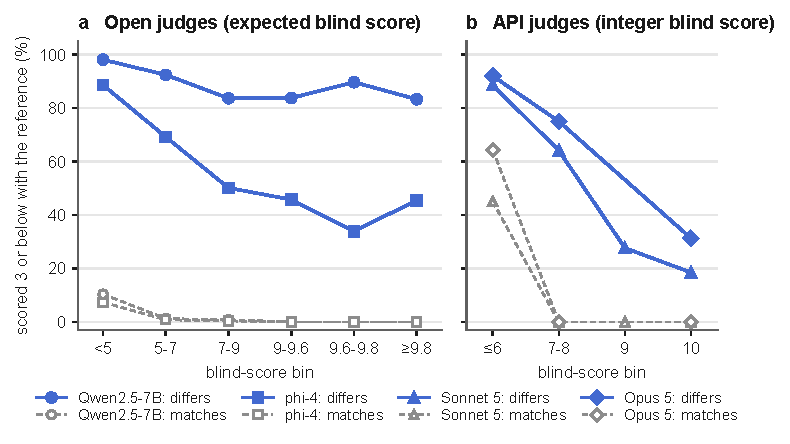
\includegraphics[width=\linewidth]{figures/figA_bins.pdf}
\caption{Rejection by blind-score bin on \textsc{MACE}: the share of correct answers scored 3 or below with the reference, for answers that differ from it (solid) and answers that match it (dashed grey). Open judges are binned on expected blind score, API judges on integer blind score; bins with at least 10 differing answers.\ph}
\label{fig:bins}
\end{figure}

\begin{table}[htbp]
\centering
\caption{Open judges: share (\%) of correct answers scored 3 or below with the reference, by blind expected score, for answers that differ from the reference and answers that match it (number of answers in parentheses).\ph}
\label{tab:r22-bins-open}
\footnotesize
\setlength{\tabcolsep}{3pt}
\begin{tabular}{llrrrrrr}
\toprule
Judge and pool & Answers & $<5$ & 5--7 & 7--9 & 9--9.6 & 9.6--9.8 & $\geq 9.8$ \\
\midrule
Qwen2.5-7B, \textsc{MACE} & differ & 98 (838) & 92 (409) & 84 (710) & 84 (203) & 90 (126) & 83 (527) \\
 & match & 10 (394) & 1 (161) & 1 (119) & 0 (63) & 0 (27) & 0 (266) \\
phi-4, \textsc{MACE} & differ & 89 (658) & 69 (711) & 50 (1578) & 46 (911) & 34 (239) & 46 (536) \\
 & match & 7 (325) & 1 (369) & 0 (531) & 0 (382) & 0 (169) & 0 (265) \\
Qwen2.5-7B, Replication & differ & 68 (81) & 42 (163) & 33 (690) & 28 (386) & 25 (253) & 19 (1747) \\
 & match & 0 (12) & 0 (39) & 1 (207) & 0 (85) & 0 (60) & 0 (466) \\
phi-4, Replication & differ & 59 (39) & 30 (103) & 10 (588) & 8 (533) & 5 (316) & 5 (1741) \\
 & match & 0 (1) & 0 (11) & 0 (136) & 0 (127) & 0 (90) & 0 (504) \\
Qwen2.5-7B, $k$-pool & differ & 72 (57) & 47 (76) & 38 (308) & 39 (154) & 28 (90) & 26 (737) \\
 & match & 0 (6) & 8 (13) & 0 (102) & 0 (50) & 0 (31) & 0 (204) \\
phi-4, $k$-pool & differ & 37 (19) & 15 (59) & 10 (332) & 8 (246) & 14 (120) & 15 (646) \\
 & match & 0 (4) & 0 (9) & 0 (66) & 0 (79) & 0 (38) & 0 (210) \\
Qwen2.5-14B, $k$-pool & differ & 78 (36) & 37 (91) & 15 (666) & 28 (116) & 39 (59) & 23 (454) \\
 & match & 20 (5) & 0 (19) & 0 (224) & 0 (34) & 0 (26) & 0 (98) \\
gemma-2-9b, $k$-pool & differ & 89 (108) & 60 (117) & 54 (473) & 55 (188) & 63 (97) & 56 (439) \\
 & match & 11 (27) & 3 (35) & 1 (145) & 0 (56) & 0 (27) & 0 (116) \\
\bottomrule
\end{tabular}

\end{table}

\begin{table}[htbp]
\centering
\caption{API judges on their 16-candidate subsamples: the same by integer blind score.\ph}
\label{tab:r22-bins-api}
\footnotesize
\begin{tabular}{llrrrr}
\toprule
Judge and pool & Answers & $\leq 6$ & 7--8 & 9 & 10 \\
\midrule
Sonnet 5, \textsc{MACE} & differ & 89 (35) & 64 (39) & 28 (94) & 19 (81) \\
 & match & 45 (20) & 0 (30) & 0 (45) & 0 (38) \\
Sonnet 5, Replication & differ & 53 (17) & 9 (45) & 15 (53) & 9 (150) \\
 & match & 0 (3) & 0 (13) & 0 (26) & 0 (60) \\
Sonnet 5, $k$-pool & differ & 75 (8) & 35 (20) & 30 (30) & 15 (87) \\
 & match & 0 (4) & 0 (9) & 0 (21) & 0 (39) \\
Opus 5, \textsc{MACE} & differ & 92 (25) & 75 (12) & 100 (5) & 31 (201) \\
 & match & 64 (14) & 0 (6) & 0 (9) & 0 (103) \\
Opus 5, Replication & differ & 50 (10) & 4 (27) & 0 (17) & 5 (211) \\
 & match & 0 (3) & 0 (5) & 0 (6) & 0 (88) \\
Opus 5, $k$-pool & differ & 25 (8) & 12 (17) & 14 (7) & 3 (113) \\
 & match & 40 (5) & 14 (7) & 0 (5) & 0 (56) \\
\bottomrule
\end{tabular}

\end{table}

\paragraph{Open judges as graders.}
Graded by Qwen2.5-7B or phi-4, Llama-3.1-8B's 64 stored samples per question on the same 150 questions are under-counted blind as well as with the reference, and with the reference these judges credit at most 1.4\% of the correct answers that differ from it (\cref{tab:r20-benchopen}).\ph{} Each judge's row uses the samples it scored in both conditions, so answer-list accuracy differs between the rows.

\begin{table}[htbp]
\centering
\caption{Open judges as graders of Llama-3.1-8B's stored samples on the 150 multi-answer \textsc{MACE} questions (a score of 7 or above counts as correct; question-level bootstrap).\ph}
\label{tab:r20-benchopen}
\footnotesize
\begin{tabular}{lrrrrr}
\toprule
Judge & List (\%) & Blind (\%) & Ref.\ (\%) & Ref.\ $-$ list & Differing credited: blind; ref. \\
\midrule
Qwen2.5-7B & 60.7 & 39.8 & 14.0 & \begin{tabular}[c]{@{}c@{}}$-46.7$\\{\scriptsize$[-52.4,-40.9]$}\end{tabular} & 55.7\%; 0.5\% \\
phi-4 & 69.5 & 54.1 & 22.1 & \begin{tabular}[c]{@{}c@{}}$-47.5$\\{\scriptsize$[-53.3,-41.5]$}\end{tabular} & 70.5\%; 1.4\% \\
\bottomrule
\end{tabular}

\end{table}

%==========================================================================================
\FloatBarrier
\section{Benchmark graders and fixes}
\label{app:r24}

\paragraph{Design.} A pre-specified experiment graded the 596 benchmark answers of Section~6 of the paper (149 \textsc{MACE} questions, one answer each from Llama-3.1-8B-Instruct, Claude Haiku~4.5, Sonnet~5, and Opus~5; 90.6\% correct by the answer lists) with two graders copied verbatim from their repositories at pinned commits: the SimpleQA grader of \texttt{openai/simple-evals}, which sends a few-shot template to GPT-4.1 (system message ``You are a helpful assistant.'', temperature 0.5) and reads a letter A (correct), B, or C, and the judge prompt of Humanity's Last Exam, which BrowseComp also uses, sent to o3-mini with HLE's structured output or to GPT-4.1 as configured for BrowseComp and read as ``correct: yes/no''. Sonnet~5 (thinking disabled) ran both prompts as a second judge. Each answer was graded with the first reference draw as the gold target and with the full answer list written as ``Any one of the following is a complete correct answer: $a_1$; $a_2$; \dots''. Every call returned a parseable grade, and the official parse and a markdown-robust parse agreed on all of them (\cref{tab:r24-standard}).

\begin{table}[htbp]
\centering
\caption{Benchmark graders with one reference and with the full answer list: pooled accuracy minus answer-list accuracy (points, 95\% CI, question bootstrap), and the share of correct answers that differ from the reference (396) and of wrong answers (56) that each condition credits. 149 questions per row.\pre}
\label{tab:r24-standard}
\footnotesize
\setlength{\tabcolsep}{3pt}
\begin{adjustbox}{max width=\linewidth}\begin{tabular}{llcccccc}
\toprule
 & & \multicolumn{2}{c}{Accuracy minus list (points)} & \multicolumn{2}{c}{Differing correct credited (\%)} & \multicolumn{2}{c}{Wrong credited (\%)} \\
\cmidrule(lr){3-4}\cmidrule(lr){5-6}\cmidrule(lr){7-8}
Prompt & Judge & One reference & Full list & One ref. & Full list & One ref. & Full list \\
\midrule
SimpleQA grader & GPT-4.1 & \begin{tabular}[c]{@{}c@{}}$-30.4$\\{\scriptsize$[-35.4,-25.3]$}\end{tabular} & \begin{tabular}[c]{@{}c@{}}$+0.3$\\{\scriptsize$[-0.7,+1.5]$}\end{tabular} & 53.0 & 99.2 & 8.9 & 8.9 \\
BrowseComp judge & GPT-4.1 & \begin{tabular}[c]{@{}c@{}}$-66.8$\\{\scriptsize$[-71.8,-61.7]$}\end{tabular} & \begin{tabular}[c]{@{}c@{}}$-0.2$\\{\scriptsize$[-0.8,+0.5]$}\end{tabular} & 0.0 & 99.2 & 0.0 & 3.6 \\
HLE judge & o3-mini & \begin{tabular}[c]{@{}c@{}}$-66.6$\\{\scriptsize$[-71.8,-61.6]$}\end{tabular} & \begin{tabular}[c]{@{}c@{}}$+0.0$\\{\scriptsize$[-0.8,+0.8]$}\end{tabular} & 0.0 & 99.2 & 0.0 & 5.4 \\
SimpleQA grader & Sonnet~5 & \begin{tabular}[c]{@{}c@{}}$-34.4$\\{\scriptsize$[-39.9,-29.2]$}\end{tabular} & \begin{tabular}[c]{@{}c@{}}$+0.5$\\{\scriptsize$[-0.3,+1.5]$}\end{tabular} & 46.7 & 99.5 & 10.7 & 8.9 \\
HLE judge & Sonnet~5 & \begin{tabular}[c]{@{}c@{}}$-64.9$\\{\scriptsize$[-70.3,-59.9]$}\end{tabular} & \begin{tabular}[c]{@{}c@{}}$+0.2$\\{\scriptsize$[-0.3,+0.7]$}\end{tabular} & 2.3 & 99.7 & 1.8 & 3.6 \\
\bottomrule
\end{tabular}
\end{adjustbox}
\end{table}

The wrong answers credited only with the full list are ``The Democratic Republic of Congo'' (listed as ``Democratic Republic of the Congo'', credited in four configurations), ``Territory of New Guinea'' (listed ``Papua New Guinea''), ``Wales'' (listed ``United Kingdom''), and ``Sudan'' (listed ``South Sudan''); the registered bound of 3 points on extra wrong-answer credit failed for the BrowseComp/HLE judge with GPT-4.1 (2 of 56) and o3-mini (3 of 56).

\paragraph{GPT-4.1 with our rubric.} GPT-4.1, with the logprob-expected score of \cref{app:frontier}, graded the same answers blind, with the first reference, and with a second reference drawn from each list (\cref{tab:r24-gpt41}). Answers that stop matching under the second draw are credited 100\% under the first and 87.5\% under the second (144 answers); answers that start matching, 80.5\% and 99.4\% (174). All four predictions were confirmed.

\begin{table}[htbp]
\centering
\caption{GPT-4.1 as a benchmark grader with our rubric: accuracy (\%) by answering model, and pooled accuracy minus the answer lists (points, 95\% CI).\pre}
\label{tab:r24-gpt41}
\footnotesize
\begin{tabular}{lcccc}
\toprule
Model & Answer list & Blind & One reference & Second reference \\
\midrule
Llama-3.1-8B & 69.1 & 63.8 & 65.8 & --- \\
Haiku~4.5 & 94.6 & 94.6 & 80.5 & --- \\
Sonnet~5 & 98.7 & 94.0 & 79.9 & --- \\
Opus~5 & 100.0 & 100.0 & 98.0 & --- \\
Pooled, minus list & & \begin{tabular}[c]{@{}c@{}}$-2.5$\\{\scriptsize$[-4.7,-0.3]$}\end{tabular} & \begin{tabular}[c]{@{}c@{}}$-9.6$\\{\scriptsize$[-12.9,-6.4]$}\end{tabular} & \begin{tabular}[c]{@{}c@{}}$-7.0$\\{\scriptsize$[-10.1,-4.0]$}\end{tabular} \\
\bottomrule
\end{tabular}

\end{table}

\paragraph{The answer list and prompt changes, measured by grading.} On the 40 \textsc{MACE} subsamples of \cref{app:frontier}, Sonnet~5, Opus~5 (their earlier blind and referenced calls reused), and GPT-4.1 graded every candidate with the full answer list in the reference slot, and Sonnet~5 with adaptive thinking graded them with one reference and the full-credit sentence, its earlier thinking blind calls reused (\cref{tab:r24-fix}). All nine answer-list predictions and two of the three combination predictions were confirmed; the combination left no measurable rise in false rejections, so its third prediction, that the rise would remain, was not confirmed.

\begin{table}[htbp]
\centering
\caption{Grading AUROC of correct answers that differ from the reference against wrong answers, blind, with one reference, and with the full answer list, and changes against blind (95\% CI, task bootstrap); below, Sonnet~5 with the full-credit sentence, adaptive thinking, and both, each against its own blind calls. 40 tasks.\pre}
\label{tab:r24-fix}
\footnotesize
\setlength{\tabcolsep}{3pt}
\begin{adjustbox}{max width=\linewidth}\begin{tabular}{lcccccc}
\toprule
 & \multicolumn{3}{c}{Grading AUROC} & \multicolumn{3}{c}{Change against blind} \\
\cmidrule(lr){2-4}\cmidrule(lr){5-7}
Judge & Blind & One ref. & Full list & One ref. & Full list & False rejections, full list (pp) \\
\midrule
Sonnet~5 & 0.938 & 0.785 & 0.970 & \begin{tabular}[c]{@{}c@{}}$-0.153$\\{\scriptsize$[-0.219,-0.097]$}\end{tabular} & \begin{tabular}[c]{@{}c@{}}$+0.032$\\{\scriptsize$[+0.008,+0.060]$}\end{tabular} & \begin{tabular}[c]{@{}c@{}}$-2.2$\\{\scriptsize$[-8.0,+4.9]$}\end{tabular} \\
Opus~5 & 0.936 & 0.771 & 0.969 & \begin{tabular}[c]{@{}c@{}}$-0.164$\\{\scriptsize$[-0.223,-0.110]$}\end{tabular} & \begin{tabular}[c]{@{}c@{}}$+0.033$\\{\scriptsize$[-0.000,+0.084]$}\end{tabular} & \begin{tabular}[c]{@{}c@{}}$-6.3$\\{\scriptsize$[-12.8,-1.1]$}\end{tabular} \\
GPT-4.1 & 0.935 & 0.872 & 0.992 & \begin{tabular}[c]{@{}c@{}}$-0.063$\\{\scriptsize$[-0.133,+0.004]$}\end{tabular} & \begin{tabular}[c]{@{}c@{}}$+0.057$\\{\scriptsize$[+0.013,+0.121]$}\end{tabular} & \begin{tabular}[c]{@{}c@{}}$-2.2$\\{\scriptsize$[-4.6,-0.5]$}\end{tabular} \\
\midrule
\multicolumn{7}{@{}l}{\emph{Sonnet~5, when the answers are not listed: change against blind}}\\
 & \multicolumn{3}{l}{Setting} & AUROC & & False rejections (pp) \\
 & \multicolumn{3}{l}{Full-credit sentence} & \begin{tabular}[c]{@{}c@{}}$-0.065$\\{\scriptsize$[-0.114,-0.019]$}\end{tabular} & & \begin{tabular}[c]{@{}c@{}}$+18.1$\\{\scriptsize$[+9.9,+28.0]$}\end{tabular} \\
 & \multicolumn{3}{l}{Adaptive thinking} & \begin{tabular}[c]{@{}c@{}}$-0.091$\\{\scriptsize$[-0.140,-0.050]$}\end{tabular} & & \begin{tabular}[c]{@{}c@{}}$+14.9$\\{\scriptsize$[+8.2,+23.1]$}\end{tabular} \\
 & \multicolumn{3}{l}{Thinking and the sentence} & \begin{tabular}[c]{@{}c@{}}$-0.024$\\{\scriptsize$[-0.062,+0.006]$}\end{tabular} & & \begin{tabular}[c]{@{}c@{}}$-0.2$\\{\scriptsize$[-7.2,+4.6]$}\end{tabular} \\
\bottomrule
\end{tabular}
\end{adjustbox}
\end{table}

%==========================================================================================
\FloatBarrier
\section{Judges that reason before deciding}
\label{app:r25}

A pre-specified experiment graded the benchmark answers of Section~6 of the paper with three prompts that ask the judge to reason about correctness, blind and with the first reference, with GPT-4.1 (temperature 0) and Sonnet~5 (thinking disabled), each allowed 1,024 output tokens; none of the prompts says whether a question can have several correct answers. \emph{Chain of thought}: ``Think step by step about whether the response is correct''. \emph{Verify first}: ``1.~Verify: using your own knowledge, check whether the response's final answer is correct for the question as asked. 2.~Compare: check the response against the reference answer. 3.~Decide whether the response is correct.'' \emph{Solve first}: ``First answer the question yourself. Then grade the response, using your own answer and the reference answer.'' Each ends with a line ``correct: yes'' or ``correct: no''; every one of the 7,152 replies had one, and none was cut off (\cref{tab:r25}). We had predicted a drop of at least 10 points in credit for differing correct answers; the drop was 0.8 to 8.6, so that prediction failed for all six.

\begin{table}[htbp]
\centering
\caption{Judges that reason before deciding, on 149 benchmark questions: pooled accuracy minus answer-list accuracy (points, 95\% CI), and the share of differing correct (396), matching correct (144), and wrong (56) answers credited blind and with the reference.\pre}
\label{tab:r25}
\footnotesize
\setlength{\tabcolsep}{3pt}
\begin{adjustbox}{max width=\linewidth}\begin{tabular}{llccccc}
\toprule
 & & \multicolumn{2}{c}{Accuracy minus list (points)} & \multicolumn{3}{c}{Credited (\%): blind $\to$ reference} \\
\cmidrule(lr){3-4}\cmidrule(lr){5-7}
Judge type & Judge & Blind & Reference & Differing correct & Matching correct & Wrong \\
\midrule
Chain of thought & GPT-4.1 & \begin{tabular}[c]{@{}c@{}}$-0.8$\\{\scriptsize$[-2.3,+0.7]$}\end{tabular} & \begin{tabular}[c]{@{}c@{}}$-3.0$\\{\scriptsize$[-4.7,-1.3]$}\end{tabular} & 97.7 $\to$ 94.7 & 98.6 $\to$ 98.6 & 10.7 $\to$ 8.9 \\
 & Sonnet~5 & \begin{tabular}[c]{@{}c@{}}$-0.5$\\{\scriptsize$[-1.8,+1.0]$}\end{tabular} & \begin{tabular}[c]{@{}c@{}}$-6.0$\\{\scriptsize$[-8.7,-3.5]$}\end{tabular} & 98.0 $\to$ 90.2 & 99.3 $\to$ 99.3 & 10.7 $\to$ 7.1 \\
Verify first & GPT-4.1 & \begin{tabular}[c]{@{}c@{}}$-0.3$\\{\scriptsize$[-1.8,+1.2]$}\end{tabular} & \begin{tabular}[c]{@{}c@{}}$-1.5$\\{\scriptsize$[-3.0,+0.0]$}\end{tabular} & 98.0 $\to$ 96.7 & 99.3 $\to$ 98.6 & 12.5 $\to$ 10.7 \\
 & Sonnet~5 & \begin{tabular}[c]{@{}c@{}}$-0.2$\\{\scriptsize$[-1.3,+1.0]$}\end{tabular} & \begin{tabular}[c]{@{}c@{}}$-6.2$\\{\scriptsize$[-8.9,-3.7]$}\end{tabular} & 98.7 $\to$ 90.2 & 99.3 $\to$ 99.3 & 8.9 $\to$ 5.4 \\
Solve first & GPT-4.1 & \begin{tabular}[c]{@{}c@{}}$-0.3$\\{\scriptsize$[-1.7,+1.0]$}\end{tabular} & \begin{tabular}[c]{@{}c@{}}$-0.5$\\{\scriptsize$[-2.0,+1.2]$}\end{tabular} & 98.2 $\to$ 97.5 & 98.6 $\to$ 100.0 & 12.5 $\to$ 12.5 \\
 & Sonnet~5 & \begin{tabular}[c]{@{}c@{}}$+0.0$\\{\scriptsize$[-1.3,+1.3]$}\end{tabular} & \begin{tabular}[c]{@{}c@{}}$-3.4$\\{\scriptsize$[-5.7,-1.2]$}\end{tabular} & 98.2 $\to$ 93.4 & 100.0 $\to$ 100.0 & 12.5 $\to$ 10.7 \\
\bottomrule
\end{tabular}
\end{adjustbox}
\end{table}

%==========================================================================================
\FloatBarrier
\section{Instruction against reasoning, grading with wrong answers, and RL verifiers}
\label{app:r26}

\paragraph{Instruction against reasoning.} A pre-specified experiment separated the instruction from written reasoning on the benchmark answers of Section~6 of the paper. GPT-4.1 (temperature 0) and Sonnet~5 (thinking disabled) graded every answer with a direct prompt, ``Is the response a correct answer to the question?'', asking for a single ``correct: yes'' or ``correct: no'' line, blind and with the reference; with the HLE judge prompt verbatim; and with the same prompt after deleting ``do not argue for any answer different than [correct\_answer], focus only on whether the answers match'' and adding ``A response that gives a different answer that is also correct for the question is correct'' (\cref{tab:r26-instruction}). All settings were the same across prompts, so the verbatim rows differ slightly from \cref{tab:r24-standard}, where GPT-4.1 ran as simple-evals configures it. Without written reasoning, accuracy with the reference falls 17.4 points below the lists for GPT-4.1 and 10.1 for Sonnet~5 (12.1 and 8.4 below blind), against 3.0 and 6.0 with chain of thought; the registered prediction that the two would be within 5 points held for Sonnet~5 and failed for GPT-4.1. Removing the match clause recovers 35.4 and 52.5 points but leaves 31.2 and 12.6, so the registered 10-point bound failed for both.

\begin{table}[htbp]
\centering
\caption{Instruction against reasoning on the benchmark pool: accuracy minus answer-list accuracy (points, 95\% CI), and the share of differing correct (396) and wrong (56) answers credited. 149 questions.\pre}
\label{tab:r26-instruction}
\footnotesize
\setlength{\tabcolsep}{3pt}
\begin{adjustbox}{max width=\linewidth}\begin{tabular}{llcccc}
\toprule
Judge & Prompt & Condition & Accuracy minus list (points) & Differing correct credited (\%) & Wrong credited (\%) \\
\midrule
GPT-4.1 & Direct yes/no & blind & \begin{tabular}[c]{@{}c@{}}$-5.4$\\{\scriptsize$[-7.7,-3.2]$}\end{tabular} & 91.4 & 12.5 \\
 & Direct yes/no & reference & \begin{tabular}[c]{@{}c@{}}$-17.4$\\{\scriptsize$[-21.0,-14.1]$}\end{tabular} & 73.2 & 7.1 \\
 & HLE judge, verbatim & reference & \begin{tabular}[c]{@{}c@{}}$-66.6$\\{\scriptsize$[-71.8,-61.6]$}\end{tabular} & 0.0 & 0.0 \\
 & HLE judge, match clause removed & reference & \begin{tabular}[c]{@{}c@{}}$-31.2$\\{\scriptsize$[-36.4,-26.3]$}\end{tabular} & 53.3 & 0.0 \\
\addlinespace
Sonnet~5 & Direct yes/no & blind & \begin{tabular}[c]{@{}c@{}}$-1.7$\\{\scriptsize$[-3.5,+0.0]$}\end{tabular} & 96.5 & 10.7 \\
 & Direct yes/no & reference & \begin{tabular}[c]{@{}c@{}}$-10.1$\\{\scriptsize$[-13.3,-6.9]$}\end{tabular} & 83.3 & 10.7 \\
 & HLE judge, verbatim & reference & \begin{tabular}[c]{@{}c@{}}$-65.1$\\{\scriptsize$[-70.3,-60.1]$}\end{tabular} & 1.8 & 3.6 \\
 & HLE judge, match clause removed & reference & \begin{tabular}[c]{@{}c@{}}$-12.6$\\{\scriptsize$[-16.3,-9.1]$}\end{tabular} & 80.3 & 7.1 \\
\bottomrule
\end{tabular}
\end{adjustbox}
\end{table}

\paragraph{Grading with many wrong answers.} On the 40 \textsc{MACE} subsamples, the same judges graded every candidate with the direct, verify-first, and solve-first prompts, blind and with the reference, and with the verbatim and edited HLE judge (\cref{tab:r26-subsample}). With the reference, grading AUROC falls 0.04 to 0.09 under every prompt; only solve-first stays within the registered 0.05 for both judges. False acceptances rise by at most 3.2 points. The verbatim HLE judge rejects 96\% to 100\% of differing correct answers, at chance AUROC; removing its match clause brings AUROC to 0.61 and 0.82. For comparison, the full answer list puts AUROC 0.03 to 0.06 above blind (\cref{tab:r24-fix}).

\begin{table}[htbp]
\centering
\caption{Grading on the 40-task \textsc{MACE} subsample: grading AUROC of differing correct answers against wrong answers, blind and with the reference, and changes in AUROC, false rejections, and false acceptances (95\% CI, task bootstrap); last row per judge: the HLE judge with its match clause removed against the verbatim judge.\pre}
\label{tab:r26-subsample}
\footnotesize
\setlength{\tabcolsep}{3pt}
\begin{adjustbox}{max width=\linewidth}\begin{tabular}{llcccc}
\toprule
Judge & Prompt & AUROC, blind $\to$ reference & AUROC change & False rejections change (pp) & False acceptances change (pp) \\
\midrule
GPT-4.1 & Direct yes/no & 0.848 $\to$ 0.759 & \begin{tabular}[c]{@{}c@{}}$-0.089$\\{\scriptsize$[-0.141,-0.038]$}\end{tabular} & \begin{tabular}[c]{@{}c@{}}$+23.0$\\{\scriptsize$[+12.3,+34.3]$}\end{tabular} & \begin{tabular}[c]{@{}c@{}}$-5.1$\\{\scriptsize$[-11.2,+0.6]$}\end{tabular} \\
 & Verify first & 0.927 $\to$ 0.859 & \begin{tabular}[c]{@{}c@{}}$-0.068$\\{\scriptsize$[-0.115,-0.026]$}\end{tabular} & \begin{tabular}[c]{@{}c@{}}$+10.3$\\{\scriptsize$[+2.7,+19.5]$}\end{tabular} & \begin{tabular}[c]{@{}c@{}}$+3.2$\\{\scriptsize$[-0.2,+7.9]$}\end{tabular} \\
 & Solve first & 0.907 $\to$ 0.868 & \begin{tabular}[c]{@{}c@{}}$-0.040$\\{\scriptsize$[-0.088,-0.002]$}\end{tabular} & \begin{tabular}[c]{@{}c@{}}$+4.7$\\{\scriptsize$[+0.4,+10.8]$}\end{tabular} & \begin{tabular}[c]{@{}c@{}}$+3.2$\\{\scriptsize$[-2.0,+9.2]$}\end{tabular} \\
 & HLE edited minus verbatim & 0.485 $\to$ 0.611 & \begin{tabular}[c]{@{}c@{}}$+0.126$\\{\scriptsize$[+0.077,+0.176]$}\end{tabular} & \begin{tabular}[c]{@{}c@{}}$-28.5$\\{\scriptsize$[-39.1,-18.1]$}\end{tabular} & \begin{tabular}[c]{@{}c@{}}$+3.4$\\{\scriptsize$[+0.0,+8.7]$}\end{tabular} \\
\addlinespace
Sonnet~5 & Direct yes/no & 0.862 $\to$ 0.805 & \begin{tabular}[c]{@{}c@{}}$-0.057$\\{\scriptsize$[-0.106,-0.014]$}\end{tabular} & \begin{tabular}[c]{@{}c@{}}$+13.8$\\{\scriptsize$[+5.8,+23.6]$}\end{tabular} & \begin{tabular}[c]{@{}c@{}}$-2.5$\\{\scriptsize$[-8.9,+3.6]$}\end{tabular} \\
 & Verify first & 0.908 $\to$ 0.818 & \begin{tabular}[c]{@{}c@{}}$-0.090$\\{\scriptsize$[-0.143,-0.041]$}\end{tabular} & \begin{tabular}[c]{@{}c@{}}$+17.1$\\{\scriptsize$[+8.3,+26.8]$}\end{tabular} & \begin{tabular}[c]{@{}c@{}}$+0.9$\\{\scriptsize$[-3.2,+4.9]$}\end{tabular} \\
 & Solve first & 0.913 $\to$ 0.867 & \begin{tabular}[c]{@{}c@{}}$-0.047$\\{\scriptsize$[-0.082,-0.016]$}\end{tabular} & \begin{tabular}[c]{@{}c@{}}$+7.4$\\{\scriptsize$[+1.7,+14.7]$}\end{tabular} & \begin{tabular}[c]{@{}c@{}}$+1.9$\\{\scriptsize$[+0.0,+5.0]$}\end{tabular} \\
 & HLE edited minus verbatim & 0.501 $\to$ 0.818 & \begin{tabular}[c]{@{}c@{}}$+0.317$\\{\scriptsize$[+0.263,+0.369]$}\end{tabular} & \begin{tabular}[c]{@{}c@{}}$-65.9$\\{\scriptsize$[-76.5,-55.2]$}\end{tabular} & \begin{tabular}[c]{@{}c@{}}$+2.5$\\{\scriptsize$[+0.3,+5.7]$}\end{tabular} \\
\bottomrule
\end{tabular}
\end{adjustbox}
\end{table}

\paragraph{Open RL-reward verifiers.} A pre-specified experiment ran two open verifiers used for RL rewards on the benchmark answers, with one reference and with the full answer list as the gold answer: General-Reasoner's \texttt{general-verifier} (1.5B) with its template and reward rule (``Final Decision: Yes''), and CompassVerifier-3B with its template (\cref{tab:r26-verifiers}). Both ran locally with greedy decoding; after three low-memory stops the runs continued in chunks (Amendment 3); to answer a status question we counted credited answers in the partial General-Reasoner output (1,011 of 1,192 generations) before the run finished, without changing any setting (registration note); and 12 General-Reasoner replies reached 512 tokens without a decision and count as incorrect. With one reference, General-Reasoner's verifier falls 62.4 points short of the lists, crediting 5.8\% of differing correct answers and 97.2\% of matching ones. With the full list it credits 67.4\% of differing correct answers but only 77.8\% of matching ones, and accepts 30.4\% of wrong answers against 8.9\%, so it stays 24.2 points short and the registered 5-point bound failed. CompassVerifier-3B, whose prompt declares the standard answer ``ALWAYS CORRECT'', credits no differing correct answer and no wrong answer with one reference (66.6 points short), and with the full list credits 99.2\% of differing correct answers and 3.6\% of wrong ones, within 0.2 points of the lists.

\begin{table}[htbp]
\centering
\caption{Open RL-reward verifiers on the benchmark answers: accuracy minus answer-list accuracy (points, 95\% CI), and the share of differing correct (396) and wrong (56) answers credited, with one reference and with the full answer list. 149 questions.\pre}
\label{tab:r26-verifiers}
\footnotesize
\setlength{\tabcolsep}{3pt}
\begin{adjustbox}{max width=\linewidth}\begin{tabular}{lcccccc}
\toprule
 & \multicolumn{2}{c}{Accuracy minus list (points)} & \multicolumn{2}{c}{Differing correct credited (\%)} & \multicolumn{2}{c}{Wrong credited (\%)} \\
\cmidrule(lr){2-3}\cmidrule(lr){4-5}\cmidrule(lr){6-7}
Verifier & One reference & Full list & One ref. & Full list & One ref. & Full list \\
\midrule
General-Reasoner verifier (1.5B) & \begin{tabular}[c]{@{}c@{}}$-62.4$\\{\scriptsize$[-67.4,-57.4]$}\end{tabular} & \begin{tabular}[c]{@{}c@{}}$-24.2$\\{\scriptsize$[-28.7,-20.0]$}\end{tabular} & 5.8 & 67.4 & 8.9 & 30.4 \\
CompassVerifier-3B & \begin{tabular}[c]{@{}c@{}}$-66.6$\\{\scriptsize$[-71.8,-61.6]$}\end{tabular} & \begin{tabular}[c]{@{}c@{}}$-0.2$\\{\scriptsize$[-0.8,+0.5]$}\end{tabular} & 0.0 & 99.2 & 0.0 & 3.6 \\
\bottomrule
\end{tabular}
\end{adjustbox}
\end{table}

%==========================================================================================
\FloatBarrier
\section{P3 under correctness prompts, and hard single-answer questions}
\label{app:r27}

\paragraph{P3 under correctness prompts.} A pre-specified re-analysis of the stored round-25 and round-26 calls on the benchmark answers asked, for each prompt that asks whether the answer is correct, how many correct answers credited blind lose credit once the reference is shown (\cref{tab:r27-p3}). Answers that differ from the reference lose credit in every cell, from 1.3\% (solve first, GPT-4.1) to 22.4\% (direct prompt, GPT-4.1); answers that match it lose credit in at most 0.7\%. The difference excludes zero in seven of eight cells. These prompts have no same-prompt second blind call, so there is no noise floor.

\begin{table}[htbp]
\centering
\caption{Correct answers credited blind that lose credit with the reference, by prompt and judge (149 questions; differing and matching answers; difference with 95\% CI, question bootstrap).\pre}
\label{tab:r27-p3}
\footnotesize
\begin{tabular}{llccc}
\toprule
Judge & Prompt & Differing (\%) & Matching (\%) & Difference (points) \\
\midrule
GPT-4.1 & Direct yes/no & 22.4 (362) & 0.0 (139) & \begin{tabular}[c]{@{}c@{}}$+22.4$\\{\scriptsize$[+17.7,+27.0]$}\end{tabular} \\
 & Chain of thought & 4.4 (387) & 0.7 (142) & \begin{tabular}[c]{@{}c@{}}$+3.7$\\{\scriptsize$[+1.3,+6.2]$}\end{tabular} \\
 & Verify first & 2.1 (388) & 0.7 (143) & \begin{tabular}[c]{@{}c@{}}$+1.4$\\{\scriptsize$[-0.7,+3.2]$}\end{tabular} \\
 & Solve first & 1.3 (389) & 0.0 (142) & \begin{tabular}[c]{@{}c@{}}$+1.3$\\{\scriptsize$[+0.3,+2.5]$}\end{tabular} \\
Sonnet~5 & Direct yes/no & 14.1 (382) & 0.0 (142) & \begin{tabular}[c]{@{}c@{}}$+14.1$\\{\scriptsize$[+10.1,+18.4]$}\end{tabular} \\
 & Chain of thought & 8.5 (388) & 0.7 (143) & \begin{tabular}[c]{@{}c@{}}$+7.8$\\{\scriptsize$[+4.4,+11.4]$}\end{tabular} \\
 & Verify first & 9.2 (391) & 0.7 (143) & \begin{tabular}[c]{@{}c@{}}$+8.5$\\{\scriptsize$[+4.7,+12.7]$}\end{tabular} \\
 & Solve first & 4.9 (389) & 0.0 (144) & \begin{tabular}[c]{@{}c@{}}$+4.9$\\{\scriptsize$[+2.6,+7.5]$}\end{tabular} \\
\bottomrule
\end{tabular}

\end{table}

\paragraph{Hard single-answer questions.} The prompts that ask whether an answer is correct were tested above on questions the judges mostly answer correctly. A pre-specified experiment asked what happens on questions beyond the judge, where the reference is its main evidence. GPT-4.1-mini and Haiku~4.5 answered the 200 text-only exact-answer HLE questions of the second prevalence audit (\cref{app:prevalence}) with HLE's official system prompt; HLE's official judge (its verbatim prompt with o3-mini and structured output) labeled the 400 answers against the HLE answer, and only 7 were labeled correct. GPT-4.1 and Sonnet~5 then graded every answer with the verbatim HLE judge (reference only) and with the direct and solve-first prompts of \cref{app:r26}, blind and with the reference. Scored questions are those whose two answers have a label and a grade in every condition (191 for GPT-4.1, 196 for Sonnet~5).

With the reference, GPT-4.1 credited 17.3\% of the wrong answers under the direct prompt and 25.9\% when it solved first, against 0\% for the verbatim HLE judge; Sonnet~5 credited 0.5\% and 1.0\% (\cref{tab:r27b}). Two of the registered bounds on this increase failed for GPT-4.1, and a recall bound failed for Sonnet~5 by one of seven answers. Blind, both prompts credited far more wrong answers (GPT-4.1 61\% to 70\%; Sonnet~5 9\% to 21\%), so on these questions the reference is the judges' main evidence, and without the instruction to match GPT-4.1, though not Sonnet~5, often overrules it. Recall rests on 7 correct answers and is not informative.

Three caveats. (i) At the registered limit of 1,024 output tokens, solve-first replies often ended before a verdict (161 of GPT-4.1's 800 calls; 342 of the 460 Sonnet~5 solve-first calls run at that limit before the amendment); a dated amendment reran them at 4,096 tokens before any outcome was computed, after which 11 and 5 calls stayed ungraded. (ii) The labels come from a judge told to match, so some credited ``wrong'' answers may be equivalent to the reference. Post hoc, restricting to wrong answers that state an answer line leaves GPT-4.1 at 15.2\% (direct) and 22.9\% (solve first); at least 40 of its 97 solve-first false acceptances end with a reply saying the reference is wrong, and in a random 10 of GPT-4.1's solve-first false acceptances that we read, most credit a different final answer after the judge's own solution disagreed with the reference. GPT-4.1 credited more wrong answers from GPT-4.1-mini than from Haiku~4.5 (direct 20.7\% against 13.9\%; solve first 35.1\% against 16.6\%), so preference for its own family may contribute, but it overruled the reference for both.\ph{} (iii) Two graders and one benchmark.

\begin{table}[htbp]
\centering
\caption{Hard single-answer questions: share of label-wrong answers credited (95\% CI, question bootstrap) and label-correct answers credited, by grader and condition.\pre}
\label{tab:r27b}
\footnotesize
\begin{tabular}{lcccc}
\toprule
 & \multicolumn{2}{c}{GPT-4.1} & \multicolumn{2}{c}{Sonnet~5} \\
\cmidrule(lr){2-3}\cmidrule(lr){4-5}
Grader & Wrong credited (\%) & Recall & Wrong credited (\%) & Recall \\
\midrule
HLE judge, verbatim (reference) & 0.0 \ci{0.0}{0.0} & 6/7 & 0.0 \ci{0.0}{0.0} & 7/7 \\
Direct, blind & 61.1 \ci{55.9}{66.1} & 3/7 & 8.8 \ci{5.5}{12.4} & 1/7 \\
Direct, reference & 17.3 \ci{13.4}{21.4} & 7/7 & 0.5 \ci{0.0}{1.3} & 7/7 \\
Solve first, blind & 69.6 \ci{64.1}{74.7} & 6/7 & 21.0 \ci{16.6}{25.9} & 3/7 \\
Solve first, reference & 25.9 \ci{21.2}{30.6} & 7/7 & 1.0 \ci{0.3}{2.1} & 6/7 \\
\bottomrule
\end{tabular}

\end{table}

%==========================================================================================
\FloatBarrier
\section{The swap under a prompt that does not instruct comparison, and a chosen reference}
\label{app:r30}

Two registered experiments answer objections the earlier text conceded without testing: that our effects
might be prompt-following, since every headline number comes from a prompt that tells the judge to use or
compare with the reference, and that the size of the benchmark shortfall is a property of drawing the
reference at random.

\paragraph{The swap under the direct prompt.}
The direct prompt of \cref{app:r26} names the reference and says nothing about what to do with it; it is the
only prompt we have with that property. We re-ran the second reference draw of \cref{app:acceptance} under
it, so the candidate text is byte-identical and only the reference moves. The draw-1 arm is the existing
run of \cref{app:r26}; only the draw-2 calls are new. Among the 318 of 596 answers whose match group changes
between draws, credit follows the reference (149 questions, 596 calls per judge, no errors):

\begin{center}\footnotesize
\begin{tabular}{llccc}
\toprule
Judge & Class ($n$) & Draw 1 & Draw 2 & Change \\
\midrule
GPT-4.1 & stop matching (144) & 0.986 & 0.722 & $-0.264$ \ci{-0.352}{-0.178} \\
 & start matching (174) & 0.718 & 0.966 & $+0.247$ \ci{+0.164}{+0.328} \\
 & matches neither (222) & 0.743 & 0.712 & $-0.032$ \ci{-0.089}{+0.027} \\
\addlinespace[2pt]
Sonnet~5 & stop matching (144) & 1.000 & 0.868 & $-0.132$ \ci{-0.198}{-0.076} \\
 & start matching (174) & 0.810 & 0.989 & $+0.178$ \ci{+0.116}{+0.248} \\
 & matches neither (222) & 0.851 & 0.793 & $-0.059$ \ci{-0.107}{-0.011} \\
\bottomrule
\end{tabular}
\end{center}

\noindent Both judges confirm that answers losing the match lose credit and answers gaining it gain credit.
Two registered predictions failed. We predicted the shift would be smaller than under our rubric, which it
is for Sonnet~5 ($-0.132$ and $+0.178$ against $-0.382$ and $+0.350$) but not for GPT-4.1, whose shift is
larger than its rubric shift of $-0.125$ and $+0.189$ (\textbf{falsified}); the two are not
instrument-matched, since the rubric is a 0--10 score thresholded at 7 and the direct prompt is a binary
yes or no, so the comparison bounds the instruction's contribution only loosely. We also predicted that
answers matching neither reference would move by at most 5 points, which holds for GPT-4.1 but not for
Sonnet~5, whose placebo moves $-5.9$ points with an interval excluding zero (\textbf{falsified}); part of
Sonnet~5's movement is therefore not specific to the reference.

\paragraph{A chosen reference instead of a drawn one.}
We rebuilt the benchmark pool with the reference chosen by two pre-specified rules: \emph{first-listed},
\textsc{MACE}'s own ordering, which uses nothing about our models, and \emph{modal}, the listed answer most
of the four answering models produce, which is the most favourable reference available. Answers, labels and
lists are unchanged; only the reference and the match groups differ.

\begin{center}\footnotesize
\setlength{\tabcolsep}{4pt}
\begin{tabular}{llccc}
\toprule
Grader & Rule & Chosen $-$ list & Chosen $-$ random & Differing correct \\
\midrule
SimpleQA, GPT-4.1 & first-listed & $-0.258$ & $+0.045$ \ci{-0.003}{+0.092} & 0.519 \\
 & modal & $-0.091$ & $+0.213$ \ci{+0.164}{+0.263} & 0.504 \\
BrowseComp/HLE, o3-mini & first-listed & $-0.562$ & $+0.104$ \ci{+0.035}{+0.173} & 0.000 \\
 & modal & $-0.203$ & $+0.463$ \ci{+0.406}{+0.522} & 0.000 \\
Our rubric, Sonnet~5$^{\ast}$ & first-listed & $-0.181$ & $+0.042$ \ci{+0.005}{+0.079} & 0.663 \\
 & modal & $-0.079$ & $+0.144$ \ci{+0.104}{+0.188} & 0.595 \\
\bottomrule
\end{tabular}
\end{center}

\noindent{\footnotesize The last column is the share of correct answers differing from the reference that the
grader credits. $^{\ast}$Sonnet~5 grades its own answers here, among those of the four answering models.
Under the random draw the shortfall is $-0.304$ for the SimpleQA grader, $-0.666$ for the BrowseComp/HLE
judge and $-0.223$ for our rubric, and the credited share is 0.530, 0.000 and 0.652 respectively.}

\noindent A chosen reference shrinks the shortfall, by 21.3 points for the SimpleQA grader and 46.3 for the
HLE judge under the modal rule, and every interval on that difference excludes zero except the SimpleQA
grader's under the first-listed rule, where it includes zero (\textbf{split}). It never removes the
shortfall: every grader stays below its answer-list accuracy under both rules.

The narrowing is largely mechanical rather than better grading, and the HLE judge shows this in its purest
form. It credits 0.000 of the correct answers that differ from its reference under every rule, so its gap
falls only because fewer answers count as differing, 121 under the modal rule against 396 under the random
draw, not because it credits any of them. Choosing a canonical reference does not repair a grader that is
told to match; it makes fewer answers differ. Across all six cells the credited share moves by 0.0 to 5.7
points where the shortfall moves by 4.2 to 46.3. The two 0.0 cells are the HLE judge, which credits no
differing correct answer under either rule and so is pinned by the very effect at issue; among the graders
that credit anything the share moves by 1.1 to 5.7 points. This is why we report the
credited share as the statistic that moved least between our two reference rules, and the accuracy gap as
the one that depends on how the reference was picked.

\paragraph{Why a reference is given at all.}
Section~7 of the paper gives the reading that connects its two prescriptions; here we record why we state it
as a reading rather than a result. No experiment here manipulates judge capability while holding the number
of correct answers fixed, and the two settings we contrast, the multi-answer factual questions of
Section~6 of the paper and the hard single-answer questions of \cref{app:r27}, differ in both at once.

%==========================================================================================
\FloatBarrier
\section{The swap under a prompt that forbids using the reference}
\label{app:r31}

Round 30 showed the swap survives a prompt that names the reference and says nothing about what to do with
it. It did not test the remaining form of the instruction-following objection: a prompt that tells the judge
\emph{not} to use the reference. This experiment does, and was registered before any call.

\paragraph{Design.} The template is byte-identical to the direct prompt of \cref{app:r26} except for one
inserted sentence: ``The reference answer is only one of several correct answers. Do not compare the response
to it, and do not treat agreeing or disagreeing with it as evidence; judge only whether the response is
itself a correct answer to the question.'' Any difference from the direct arm is therefore attributable to
the instruction rather than to rewording. Both draws are new, since this template had never been run. Four
cells of 596 calls, no errors and no unparseable replies.

\begin{center}\footnotesize
\begin{tabular}{llccc}
\toprule
Judge & Class ($n$) & Draw 1 & Draw 2 & Change \\
\midrule
Sonnet~5 & stop matching (144) & 0.986 & 0.979 & $-0.007$ \ci{-0.031}{+0.015} \\
 & start matching (174) & 0.977 & 0.989 & $+0.012$ \ci{-0.011}{+0.034} \\
 & matches neither (222) & 0.968 & 0.946 & $-0.023$ \ci{-0.050}{+0.004} \\
\addlinespace[2pt]
GPT-4.1 & stop matching (144) & 0.993 & 0.972 & $-0.021$ \ci{-0.051}{+0.007} \\
 & start matching (174) & 0.977 & 0.977 & $+0.000$ \ci{-0.016}{+0.018} \\
 & matches neither (222) & 0.968 & 0.968 & $+0.000$ \ci{-0.012}{+0.013} \\
\bottomrule
\end{tabular}
\end{center}

\noindent The swap does not survive. Every interval includes zero, so both registered directional predictions
are \textbf{not confirmed} for both judges. Against the direct prompt on the same answers, GPT-4.1's
stop-matching shift falls from $-0.264$ to $-0.021$ and its start-matching shift from $+0.247$ to $+0.000$;
Sonnet~5's fall from $-0.132$ and $+0.178$ to $-0.007$ and $+0.012$. We registered that the shift would be
smaller than each judge's own shift under the direct prompt, and it is, by a wide margin (confirmed for both
judges in both directions); the placebo moves at most 2.3 points (confirmed).

\paragraph{The judges did not simply become permissive.} That is the reading this result has to survive, and
it does not hold: wrong answers are still rejected, while credit for correct answers rises sharply against
the direct prompt on the same pool.

\begin{center}\footnotesize
\begin{tabular}{lccc}
\toprule
Judge & Prompt & Correct credited & Wrong credited \\
\midrule
Sonnet~5 & direct & 0.878 & 0.107 \\
 & forbidden (draw 1 / 2) & 0.976 / 0.969 & 0.107 / 0.125 \\
\addlinespace[2pt]
GPT-4.1 & direct & 0.800 & 0.071 \\
 & forbidden (draw 1 / 2) & 0.978 / 0.972 & 0.196 / 0.214 \\
\bottomrule
\end{tabular}
\end{center}

\noindent Accuracy lands within 0.2 to 1.7 points of answer-list accuracy in every cell, against the 30 to 67
points by which the shipped graders fall short (Section~6 of the paper). The cost differs by judge: close to
free for Sonnet~5, and a real rise in wrong answers credited for GPT-4.1.

\paragraph{What this does and does not settle.} It does not make the effect an artifact of our wording:
\cref{app:r30} already shows the swap is large under a prompt that names the reference and gives no
instruction about it. Read together, the two results bound the effect from both sides. It does not require an
instruction to compare, and it does not survive one forbidding it.

%==========================================================================================
\FloatBarrier
\section{Mitigations in full}
\label{app:mitigation}

\begin{table}[htbp]
\centering
\footnotesize
\caption{\textbf{What helps: a full-credit sentence reduces the grading harm; an exploratory max rule restores grading at a cost when the answer is unique.} Change against blind judging, except \emph{Reveal $-$ ref.}, which is the registered blind-then-reveal protocol (score blind, then rescore with the reference and an instruction to keep the blind score unless the reference shows the answer is wrong) minus the reference, both with the original scorer. \emph{Sentence}: the full-credit instruction of Section~7 of the paper. Bold: the Sentence and Max rule cells differ from the Reference cell, and Reveal $-$ ref.\ differs from zero (95\% intervals); ---: not run or not defined. Task counts are in \cref{app:mitigation}. Pre-specified: the API judges' Reference and Sentence values, Qwen2.5-7B's \textsc{MACE} Reference grading, and \textsc{MACE} Reference accuracy (the original scorer gives the same values); MATH-500 Reference accuracy is a re-analysis; every Reveal $-$ ref.\ and Max rule value, and the rest, is post hoc.}
\label{tab:protocols}
\setlength{\tabcolsep}{3.1pt}
\begin{tabular}{@{}llrrrrrr@{}}
\toprule
& & \multicolumn{4}{c}{Grading AUROC} & \multicolumn{2}{c}{Accuracy (pp)} \\
\cmidrule(lr){3-6}\cmidrule(lr){7-8}
Pool & Judge & Reference & Sentence & Reveal $-$ ref. & Max rule & Reference & Max rule \\
\midrule
\multicolumn{8}{@{}l}{\emph{Several correct answers}}\\
\textsc{MACE} & Sonnet~5 & $-0.15$ & $\mathbf{-0.06}$ & --- & $\mathbf{-0.01}$ & --- & --- \\
 & Opus~5 & $-0.16$ & $\mathbf{-0.05}$ & --- & $\mathbf{-0.01}$ & --- & --- \\
 & Qwen2.5-7B & $-0.08$ & --- & $0.00$ & $\mathbf{-0.01}$ & $+2.0$ & $+4.0$ \\
 & phi-4 & $-0.06$ & --- & $+0.01$ & $\mathbf{-0.01}$ & $+6.1$ & $+6.1$ \\
$k$-pool, $k{>}1$ & Qwen2.5-7B & $-0.23$ & --- & $\mathbf{+0.11}$ & $\mathbf{+0.00}$ & $-30.3$ & $\mathbf{+3.0}$ \\
 & Qwen2.5-14B & $-0.17$ & --- & $\mathbf{+0.12}$ & $\mathbf{-0.03}$ & $-3.0$ & $+3.0$ \\
 & gemma-2-9b & $-0.19$ & --- & $\mathbf{-0.06}$ & $\mathbf{+0.00}$ & $-3.0$ & $+0.0$ \\
 & phi-4 & $-0.25$ & --- & $\mathbf{+0.04}$ & $\mathbf{-0.01}$ & $-15.2$ & $\mathbf{+3.0}$ \\
\multicolumn{8}{@{}l}{\emph{One correct answer}}\\
MATH-500, answer & Qwen2.5-7B & $+0.29$ & --- & --- & $\mathbf{+0.24}$ & $+28.6$ & $\mathbf{+23.8}$ \\
 & Qwen2.5-14B & $+0.25$ & --- & --- & $\mathbf{+0.22}$ & $+30.6$ & $+29.7$ \\
MATH-500, solution & Qwen2.5-7B & $+0.29$ & --- & $\mathbf{-0.04}$ & $\mathbf{+0.13}$ & $+30.5$ & $\mathbf{+23.8}$ \\
\bottomrule
\end{tabular}
\end{table}

\begin{figure}[htbp]
\centering
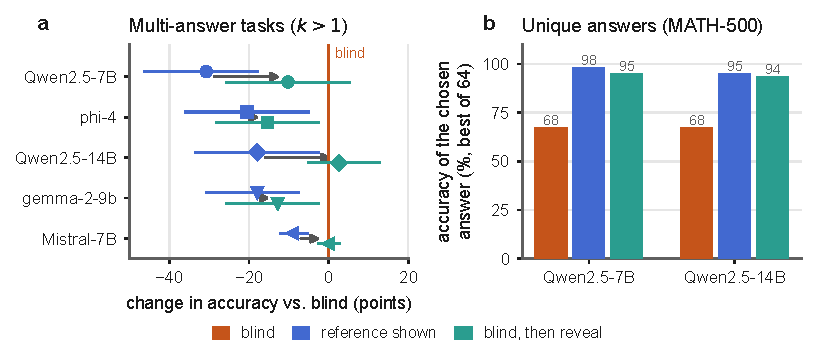
\includegraphics[width=\textwidth]{figures/fig4_fix.pdf}
\caption{\textbf{Blind-then-reveal, original scorer.} \textbf{(a)}~Change in selection accuracy relative to blind judging (orange line) on the $k$-pool at $k{>}1$, with the reference shown (blue) and with blind-then-reveal (teal); arrows run from one to the other. 39 tasks, 95\% intervals.\ph{} \textbf{(b)}~Selection accuracy on 105 MATH-500 problems with the reference solution, best of 64.\pre}
\label{fig:fix}
\end{figure}

\paragraph{Instructions and several references.}
On the synthetic grid at $k{=}16$, the any-valid-answer instruction closes phi-4's margin ($+1.91 \to +0.03$), shrinks Qwen2.5-14B's ($+3.34 \to +1.21$), and does little or nothing for smaller judges, even raising Qwen2.5-1.5B's on rubric~$a$ ($+3.58 \to +4.54$). Showing $\min(3,k)$ valid references removes the margin toward the original reference on the Qwen-generated grid without restoring blind-level inflation, and largely fails for Qwen2.5-7B on the Llama-generated grid.

\paragraph{Worked references.}
With a short worked solution in the reference slot on the $k$-pool, the margin falls from $+5.17$ to $+3.73$ (Qwen2.5-7B) and from $+4.20$ to $+3.67$ (phi-4), and added inflation falls from $+1.50$ to $+1.08$ and from $+1.07$ to $+0.77$.

\paragraph{Blind-then-reveal on unique answers.}
A later pre-specified experiment ran blind-then-reveal on the 105 MATH-500 problems (\cref{tab:r2a}). The first call reproduces the frozen blind scores ($r=0.991$ and $0.973$), so the comparison is on aligned data.

\begin{table}[htbp]
\centering
\caption{MATH-500 selection accuracy under three protocols, best of 64, rubric-$a$ selection. The blind-then-reveal comparisons were pre-specified; after a disclosed amendment, the reference-versus-blind contrast carries no registration weight (\cref{tab:ledger}).}
\label{tab:r2a}
\footnotesize
\begin{adjustbox}{max width=\linewidth}\begin{tabular}{lccccc}
\toprule
Judge & Blind & Reference & Blind, then reveal & Reveal minus reference (points) & Call-1 vs.\ frozen blind $r$ \\
\midrule
Qwen2.5-7B & 67.6\% & 98.1\% & 95.2\% & $-2.9$ {\scriptsize$[-8.6,+1.9]$} & 0.991 \\
Qwen2.5-14B & 67.6\% & 95.2\% & 93.5\% & $-1.7$ {\scriptsize$[-7.3,+3.3]$} & 0.973 \\
\bottomrule
\end{tabular}
\end{adjustbox}

\end{table}

\paragraph{Zero-cost score combinations.}
Simple combinations of the blind and referenced scores compete with blind-then-reveal (\cref{tab:score-rules}). Taking the maximum loses nothing to blind judging on the $k$-pool at $k{>}1$ and keeps the reference's benefit on \textsc{MACE}, but on MATH-500 it trails the reference for Qwen2.5-7B; the mean does best on MATH-500 and worse on the $k$-pool. No rule is best everywhere. Computed from the same stored scores, the max rule also keeps grading AUROC within 0.03 of blind judging, where showing the reference lowers it by 0.06 to 0.25; blind-then-reveal does not, except for Qwen2.5-14B (\cref{tab:protocol-grading}).\ph

\begin{table}[htbp]
\centering
\footnotesize
\caption{Best-of-64 accuracy change against blind judging (points) for score combinations and blind-then-reveal: $k$-pool at $k{>}1$ (registered labels, 39 tasks), \textsc{MACE} overall, MATH-500. Original scorer. \Cref{tab:protocols} uses any-format labels for the $k$-pool.\ph}
\label{tab:score-rules}
\begin{adjustbox}{max width=\linewidth}\begin{tabular}{lcccccccc}
\toprule
Rule & $k$-pool, 7B & $k$-pool, phi-4 & $k$-pool, 14B & $k$-pool, gemma & \textsc{MACE}, 7B & \textsc{MACE}, phi-4 & MATH, 7B & MATH, 14B \\
\midrule
Reference & $-30.8$ & $-20.5$ & $-17.9$ & $-17.9$ & $+9.8$ & $+11.3$ & $+30.5$ & $+27.6$ \\
Mean & $-7.7$ & $-17.9$ & $-2.6$ & $-15.4$ & $+6.8$ & $+7.5$ & $+32.4$ & $+30.5$ \\
Min & $-17.9$ & $-20.5$ & $-7.7$ & $-15.4$ & $+3.8$ & $+7.5$ & $+32.4$ & $+28.6$ \\
Max & $+0.0$ & $+2.6$ & $-2.6$ & $+0.0$ & $+9.8$ & $+11.3$ & $+23.8$ & $+27.6$ \\
Blind, reference breaks ties & $+0.0$ & $+0.0$ & $+0.0$ & $+0.0$ & $+1.5$ & $+0.0$ & $+10.5$ & $+4.8$ \\
Blind, then reveal & $-10.3$ & $-15.4$ & $+2.6$ & $-12.8$ & $+6.8$ & $+9.8$ & $+27.6$ & $+25.9$ \\
\bottomrule
\end{tabular}
\end{adjustbox}
\end{table}

\begin{table}[htbp]
\centering
\footnotesize
\caption{\textbf{The max rule nearly removes the grading harm; blind-then-reveal mostly does not.} Top: change in per-task grading AUROC relative to blind judging (95\% CI), for correct answers that differ from the reference against wrong answers ($k$-pool with any-format labels, 59 tasks; \textsc{MACE}, 91 tasks), and for all correct answers against wrong answers on single-answer questions. Bottom: change in best-of-64 accuracy relative to the referenced judge (points, 95\% CI). Both blocks use the original scorer, as the reveal calls did. From stored scores.\ph}
\label{tab:protocol-grading}
\begin{adjustbox}{max width=\linewidth}\begin{tabular}{llccc}
\toprule
Pool & Judge & Reference & Max rule & Blind, then reveal \\
\midrule
$k$-pool, $k{>}1$ & Qwen2.5-7B & \begin{tabular}[c]{@{}c@{}}$-0.22$\\{\scriptsize$[-0.27,-0.17]$}\end{tabular} & \begin{tabular}[c]{@{}c@{}}$+0.00$\\{\scriptsize$[-0.01,+0.01]$}\end{tabular} & \begin{tabular}[c]{@{}c@{}}$-0.11$\\{\scriptsize$[-0.15,-0.07]$}\end{tabular} \\
 & Qwen2.5-14B & \begin{tabular}[c]{@{}c@{}}$-0.13$\\{\scriptsize$[-0.17,-0.09]$}\end{tabular} & \begin{tabular}[c]{@{}c@{}}$-0.02$\\{\scriptsize$[-0.04,-0.01]$}\end{tabular} & \begin{tabular}[c]{@{}c@{}}$-0.01$\\{\scriptsize$[-0.02,+0.00]$}\end{tabular} \\
 & gemma-2-9b & \begin{tabular}[c]{@{}c@{}}$-0.18$\\{\scriptsize$[-0.21,-0.14]$}\end{tabular} & \begin{tabular}[c]{@{}c@{}}$+0.00$\\{\scriptsize$[+0.00,+0.00]$}\end{tabular} & \begin{tabular}[c]{@{}c@{}}$-0.23$\\{\scriptsize$[-0.28,-0.19]$}\end{tabular} \\
 & phi-4 & \begin{tabular}[c]{@{}c@{}}$-0.25$\\{\scriptsize$[-0.29,-0.20]$}\end{tabular} & \begin{tabular}[c]{@{}c@{}}$-0.01$\\{\scriptsize$[-0.02,+0.00]$}\end{tabular} & \begin{tabular}[c]{@{}c@{}}$-0.20$\\{\scriptsize$[-0.25,-0.15]$}\end{tabular} \\
\addlinespace
\textsc{MACE}, $k{>}1$ & Qwen2.5-7B & \begin{tabular}[c]{@{}c@{}}$-0.08$\\{\scriptsize$[-0.14,-0.01]$}\end{tabular} & \begin{tabular}[c]{@{}c@{}}$-0.01$\\{\scriptsize$[-0.03,+0.00]$}\end{tabular} & \begin{tabular}[c]{@{}c@{}}$-0.08$\\{\scriptsize$[-0.12,-0.04]$}\end{tabular} \\
 & phi-4 & \begin{tabular}[c]{@{}c@{}}$-0.06$\\{\scriptsize$[-0.10,-0.02]$}\end{tabular} & \begin{tabular}[c]{@{}c@{}}$-0.01$\\{\scriptsize$[-0.02,+0.00]$}\end{tabular} & \begin{tabular}[c]{@{}c@{}}$-0.05$\\{\scriptsize$[-0.10,-0.01]$}\end{tabular} \\
\midrule
\textsc{MACE}, $k{=}1$ (all correct) & Qwen2.5-7B & \begin{tabular}[c]{@{}c@{}}$+0.28$\\{\scriptsize$[+0.18,+0.39]$}\end{tabular} & \begin{tabular}[c]{@{}c@{}}$+0.22$\\{\scriptsize$[+0.13,+0.31]$}\end{tabular} & \begin{tabular}[c]{@{}c@{}}$+0.14$\\{\scriptsize$[+0.07,+0.22]$}\end{tabular} \\
 & phi-4 & \begin{tabular}[c]{@{}c@{}}$+0.23$\\{\scriptsize$[+0.14,+0.34]$}\end{tabular} & \begin{tabular}[c]{@{}c@{}}$+0.21$\\{\scriptsize$[+0.12,+0.31]$}\end{tabular} & \begin{tabular}[c]{@{}c@{}}$+0.23$\\{\scriptsize$[+0.14,+0.34]$}\end{tabular} \\
MATH-500 (all correct) & Qwen2.5-7B & \begin{tabular}[c]{@{}c@{}}$+0.29$\\{\scriptsize$[+0.25,+0.33]$}\end{tabular} & \begin{tabular}[c]{@{}c@{}}$+0.14$\\{\scriptsize$[+0.12,+0.17]$}\end{tabular} & \begin{tabular}[c]{@{}c@{}}$+0.25$\\{\scriptsize$[+0.21,+0.29]$}\end{tabular} \\
 & Qwen2.5-14B & \begin{tabular}[c]{@{}c@{}}$+0.30$\\{\scriptsize$[+0.26,+0.33]$}\end{tabular} & \begin{tabular}[c]{@{}c@{}}$+0.26$\\{\scriptsize$[+0.23,+0.29]$}\end{tabular} & \begin{tabular}[c]{@{}c@{}}$+0.22$\\{\scriptsize$[+0.19,+0.25]$}\end{tabular} \\
\bottomrule
\end{tabular}
\end{adjustbox}\\[6pt]
\begin{adjustbox}{max width=\linewidth}\begin{tabular}{llcc}
\toprule
Pool & Judge & Max rule $-$ reference & Blind, then reveal $-$ reference \\
\midrule
MATH-500 & Qwen2.5-7B & \begin{tabular}[c]{@{}c@{}}$-6.7$\\{\scriptsize$[-12.4,-1.9]$}\end{tabular} & \begin{tabular}[c]{@{}c@{}}$-2.9$\\{\scriptsize$[-7.6,+1.9]$}\end{tabular} \\
MATH-500 & Qwen2.5-14B & \begin{tabular}[c]{@{}c@{}}$+0.0$\\{\scriptsize$[+0.0,+0.0]$}\end{tabular} & \begin{tabular}[c]{@{}c@{}}$-1.7$\\{\scriptsize$[-7.3,+3.3]$}\end{tabular} \\
\addlinespace
$k$-pool, $k{>}1$, any format & Qwen2.5-7B & \begin{tabular}[c]{@{}c@{}}$+27.3$\\{\scriptsize$[+9.1,+45.5]$}\end{tabular} & \begin{tabular}[c]{@{}c@{}}$+24.2$\\{\scriptsize$[+9.1,+42.4]$}\end{tabular} \\
 & Qwen2.5-14B & \begin{tabular}[c]{@{}c@{}}$+3.0$\\{\scriptsize$[+0.0,+9.1]$}\end{tabular} & \begin{tabular}[c]{@{}c@{}}$+3.0$\\{\scriptsize$[-6.1,+15.2]$}\end{tabular} \\
 & gemma-2-9b & \begin{tabular}[c]{@{}c@{}}$+3.0$\\{\scriptsize$[+0.0,+9.1]$}\end{tabular} & \begin{tabular}[c]{@{}c@{}}$+3.0$\\{\scriptsize$[+0.0,+9.1]$}\end{tabular} \\
 & phi-4 & \begin{tabular}[c]{@{}c@{}}$+18.2$\\{\scriptsize$[+6.1,+33.3]$}\end{tabular} & \begin{tabular}[c]{@{}c@{}}$+9.1$\\{\scriptsize$[+0.0,+18.2]$}\end{tabular} \\
\bottomrule
\end{tabular}
\end{adjustbox}
\end{table}

\begin{table}[htbp]
\centering
\footnotesize
\caption{The reference and the max rule under the exact scorer, changes against blind judging (95\% CI); the values quoted in \cref{tab:protocols}. From stored scores.\ph}
\label{tab:protocol-exact}
\begin{adjustbox}{max width=\linewidth}\begin{tabular}{llcccccc}
\toprule
 & & \multicolumn{3}{c}{Best-of-64 accuracy (points)} & \multicolumn{3}{c}{Grading AUROC} \\
\cmidrule(lr){3-5}\cmidrule(lr){6-8}
Pool & Judge & Reference & Max rule & Max $-$ reference & Reference & Max rule & Max $-$ reference \\
\midrule
$k$-pool, $k{>}1$, any format & Qwen2.5-7B & \begin{tabular}[c]{@{}c@{}}$-30.3$\\{\scriptsize$[-48.5,-12.1]$}\end{tabular} & \begin{tabular}[c]{@{}c@{}}$+3.0$\\{\scriptsize$[+0.0,+9.1]$}\end{tabular} & \begin{tabular}[c]{@{}c@{}}$+33.3$\\{\scriptsize$[+18.2,+51.5]$}\end{tabular} & \begin{tabular}[c]{@{}c@{}}$-0.23$\\{\scriptsize$[-0.28,-0.19]$}\end{tabular} & \begin{tabular}[c]{@{}c@{}}$+0.00$\\{\scriptsize$[-0.01,+0.01]$}\end{tabular} & \begin{tabular}[c]{@{}c@{}}$+0.23$\\{\scriptsize$[+0.19,+0.27]$}\end{tabular} \\
 & Qwen2.5-14B & \begin{tabular}[c]{@{}c@{}}$-3.0$\\{\scriptsize$[-18.2,+9.1]$}\end{tabular} & \begin{tabular}[c]{@{}c@{}}$+3.0$\\{\scriptsize$[-6.1,+12.1]$}\end{tabular} & \begin{tabular}[c]{@{}c@{}}$+6.1$\\{\scriptsize$[+0.0,+15.2]$}\end{tabular} & \begin{tabular}[c]{@{}c@{}}$-0.17$\\{\scriptsize$[-0.21,-0.14]$}\end{tabular} & \begin{tabular}[c]{@{}c@{}}$-0.03$\\{\scriptsize$[-0.05,-0.01]$}\end{tabular} & \begin{tabular}[c]{@{}c@{}}$+0.14$\\{\scriptsize$[+0.11,+0.18]$}\end{tabular} \\
 & gemma-2-9b & \begin{tabular}[c]{@{}c@{}}$-3.0$\\{\scriptsize$[-9.1,+0.0]$}\end{tabular} & \begin{tabular}[c]{@{}c@{}}$+0.0$\\{\scriptsize$[+0.0,+0.0]$}\end{tabular} & \begin{tabular}[c]{@{}c@{}}$+3.0$\\{\scriptsize$[+0.0,+9.1]$}\end{tabular} & \begin{tabular}[c]{@{}c@{}}$-0.19$\\{\scriptsize$[-0.22,-0.15]$}\end{tabular} & \begin{tabular}[c]{@{}c@{}}$+0.00$\\{\scriptsize$[-0.01,+0.00]$}\end{tabular} & \begin{tabular}[c]{@{}c@{}}$+0.18$\\{\scriptsize$[+0.15,+0.22]$}\end{tabular} \\
 & phi-4 & \begin{tabular}[c]{@{}c@{}}$-15.2$\\{\scriptsize$[-30.3,+0.0]$}\end{tabular} & \begin{tabular}[c]{@{}c@{}}$+3.0$\\{\scriptsize$[+0.0,+9.1]$}\end{tabular} & \begin{tabular}[c]{@{}c@{}}$+18.2$\\{\scriptsize$[+6.1,+33.3]$}\end{tabular} & \begin{tabular}[c]{@{}c@{}}$-0.25$\\{\scriptsize$[-0.29,-0.20]$}\end{tabular} & \begin{tabular}[c]{@{}c@{}}$-0.01$\\{\scriptsize$[-0.02,+0.00]$}\end{tabular} & \begin{tabular}[c]{@{}c@{}}$+0.24$\\{\scriptsize$[+0.20,+0.28]$}\end{tabular} \\
\addlinespace
\textsc{MACE} (accuracy: natural mix; AUROC: $k{>}1$) & Qwen2.5-7B & \begin{tabular}[c]{@{}c@{}}$+9.0$\\{\scriptsize$[+2.3,+15.8]$}\end{tabular} & \begin{tabular}[c]{@{}c@{}}$+9.8$\\{\scriptsize$[+5.3,+15.0]$}\end{tabular} & \begin{tabular}[c]{@{}c@{}}$+0.8$\\{\scriptsize$[-3.8,+6.0]$}\end{tabular} & \begin{tabular}[c]{@{}c@{}}$-0.08$\\{\scriptsize$[-0.14,-0.01]$}\end{tabular} & \begin{tabular}[c]{@{}c@{}}$-0.01$\\{\scriptsize$[-0.02,+0.00]$}\end{tabular} & \begin{tabular}[c]{@{}c@{}}$+0.07$\\{\scriptsize$[+0.01,+0.13]$}\end{tabular} \\
 & phi-4 & \begin{tabular}[c]{@{}c@{}}$+11.3$\\{\scriptsize$[+4.5,+18.1]$}\end{tabular} & \begin{tabular}[c]{@{}c@{}}$+11.3$\\{\scriptsize$[+6.0,+17.3]$}\end{tabular} & \begin{tabular}[c]{@{}c@{}}$+0.0$\\{\scriptsize$[-3.8,+3.8]$}\end{tabular} & \begin{tabular}[c]{@{}c@{}}$-0.06$\\{\scriptsize$[-0.10,-0.02]$}\end{tabular} & \begin{tabular}[c]{@{}c@{}}$-0.01$\\{\scriptsize$[-0.02,+0.00]$}\end{tabular} & \begin{tabular}[c]{@{}c@{}}$+0.05$\\{\scriptsize$[+0.01,+0.09]$}\end{tabular} \\
\textsc{MACE} $k{>}1$, accuracy & Qwen2.5-7B & \begin{tabular}[c]{@{}c@{}}$+2.0$\\{\scriptsize$[-5.1,+9.1]$}\end{tabular} & \begin{tabular}[c]{@{}c@{}}$+4.0$\\{\scriptsize$[+1.0,+8.1]$}\end{tabular} & \begin{tabular}[c]{@{}c@{}}$+2.0$\\{\scriptsize$[-4.0,+8.1]$}\end{tabular} & --- & --- & --- \\
\textsc{MACE} $k{>}1$, accuracy & phi-4 & \begin{tabular}[c]{@{}c@{}}$+6.1$\\{\scriptsize$[-1.0,+13.1]$}\end{tabular} & \begin{tabular}[c]{@{}c@{}}$+6.1$\\{\scriptsize$[+2.0,+11.1]$}\end{tabular} & \begin{tabular}[c]{@{}c@{}}$+0.0$\\{\scriptsize$[-5.1,+5.1]$}\end{tabular} & --- & --- & --- \\
\textsc{MACE} $k{=}1$, all correct & Qwen2.5-7B & --- & --- & --- & \begin{tabular}[c]{@{}c@{}}$+0.29$\\{\scriptsize$[+0.19,+0.41]$}\end{tabular} & \begin{tabular}[c]{@{}c@{}}$+0.23$\\{\scriptsize$[+0.14,+0.32]$}\end{tabular} & \begin{tabular}[c]{@{}c@{}}$-0.07$\\{\scriptsize$[-0.11,-0.03]$}\end{tabular} \\
\textsc{MACE} $k{=}1$, all correct & phi-4 & --- & --- & --- & \begin{tabular}[c]{@{}c@{}}$+0.23$\\{\scriptsize$[+0.14,+0.34]$}\end{tabular} & \begin{tabular}[c]{@{}c@{}}$+0.21$\\{\scriptsize$[+0.12,+0.31]$}\end{tabular} & \begin{tabular}[c]{@{}c@{}}$-0.02$\\{\scriptsize$[-0.04,-0.01]$}\end{tabular} \\
\addlinespace
MATH-500, final answer & Qwen2.5-7B & \begin{tabular}[c]{@{}c@{}}$+28.6$\\{\scriptsize$[+18.1,+38.1]$}\end{tabular} & \begin{tabular}[c]{@{}c@{}}$+23.8$\\{\scriptsize$[+14.3,+33.3]$}\end{tabular} & \begin{tabular}[c]{@{}c@{}}$-4.8$\\{\scriptsize$[-9.5,-0.9]$}\end{tabular} & \begin{tabular}[c]{@{}c@{}}$+0.29$\\{\scriptsize$[+0.25,+0.33]$}\end{tabular} & \begin{tabular}[c]{@{}c@{}}$+0.24$\\{\scriptsize$[+0.20,+0.28]$}\end{tabular} & \begin{tabular}[c]{@{}c@{}}$-0.05$\\{\scriptsize$[-0.07,-0.03]$}\end{tabular} \\
MATH-500, solution & Qwen2.5-7B & \begin{tabular}[c]{@{}c@{}}$+30.5$\\{\scriptsize$[+21.9,+39.1]$}\end{tabular} & \begin{tabular}[c]{@{}c@{}}$+23.8$\\{\scriptsize$[+15.2,+32.4]$}\end{tabular} & \begin{tabular}[c]{@{}c@{}}$-6.7$\\{\scriptsize$[-11.4,-1.9]$}\end{tabular} & \begin{tabular}[c]{@{}c@{}}$+0.29$\\{\scriptsize$[+0.24,+0.33]$}\end{tabular} & \begin{tabular}[c]{@{}c@{}}$+0.13$\\{\scriptsize$[+0.11,+0.16]$}\end{tabular} & \begin{tabular}[c]{@{}c@{}}$-0.15$\\{\scriptsize$[-0.19,-0.12]$}\end{tabular} \\
MATH-500, final answer & Qwen2.5-14B & \begin{tabular}[c]{@{}c@{}}$+30.6$\\{\scriptsize$[+21.9,+39.4]$}\end{tabular} & \begin{tabular}[c]{@{}c@{}}$+29.7$\\{\scriptsize$[+21.1,+39.1]$}\end{tabular} & \begin{tabular}[c]{@{}c@{}}$-0.9$\\{\scriptsize$[-2.9,+0.0]$}\end{tabular} & \begin{tabular}[c]{@{}c@{}}$+0.25$\\{\scriptsize$[+0.21,+0.28]$}\end{tabular} & \begin{tabular}[c]{@{}c@{}}$+0.22$\\{\scriptsize$[+0.18,+0.25]$}\end{tabular} & \begin{tabular}[c]{@{}c@{}}$-0.03$\\{\scriptsize$[-0.04,-0.02]$}\end{tabular} \\
MATH-500, solution & Qwen2.5-14B & \begin{tabular}[c]{@{}c@{}}$+28.6$\\{\scriptsize$[+19.0,+38.1]$}\end{tabular} & \begin{tabular}[c]{@{}c@{}}$+28.6$\\{\scriptsize$[+19.0,+38.1]$}\end{tabular} & \begin{tabular}[c]{@{}c@{}}$+0.0$\\{\scriptsize$[+0.0,+0.0]$}\end{tabular} & \begin{tabular}[c]{@{}c@{}}$+0.24$\\{\scriptsize$[+0.20,+0.28]$}\end{tabular} & \begin{tabular}[c]{@{}c@{}}$+0.20$\\{\scriptsize$[+0.17,+0.24]$}\end{tabular} & \begin{tabular}[c]{@{}c@{}}$-0.04$\\{\scriptsize$[-0.05,-0.03]$}\end{tabular} \\
\bottomrule
\end{tabular}
\end{adjustbox}
\end{table}

\begin{table}[htbp]
\centering
\footnotesize
\caption{Worst-case selection loss by protocol: accuracy of each protocol minus the best of the three in each pool (points; 0 marks the best), and the worst case over the pools each judge was run on, which differ by judge. Original scorer; registered labels, which count most prose answers as wrong (\cref{app:grid}).\ph}
\label{tab:regret}
\begin{adjustbox}{max width=\linewidth}\begin{tabular}{llccc}
\toprule
Judge & Pool & Blind & Reference & Blind, then reveal \\
\midrule
Qwen2.5-7B & $k$-pool, $k{>}1$ & $+0.0$ & $-30.8$ & $-10.2$ \\
 & MATH-500 & $-30.5$ & $+0.0$ & $-2.9$ \\
 & \textsc{MACE} & $-9.8$ & $+0.0$ & $-3.0$ \\
 & \emph{worst case} & $\mathbf{-30.5}$ & $\mathbf{-30.8}$ & $\mathbf{-10.2}$ \\
\addlinespace
phi-4 & $k$-pool, $k{>}1$ & $+0.0$ & $-20.5$ & $-15.4$ \\
 & \textsc{MACE} & $-11.3$ & $+0.0$ & $-1.5$ \\
 & \emph{worst case} & $\mathbf{-11.3}$ & $\mathbf{-20.5}$ & $\mathbf{-15.4}$ \\
\addlinespace
Qwen2.5-14B & $k$-pool, $k{>}1$ & $-2.6$ & $-20.5$ & $+0.0$ \\
 & MATH-500 & $-27.6$ & $+0.0$ & $-1.7$ \\
 & \emph{worst case} & $\mathbf{-27.6}$ & $\mathbf{-20.5}$ & $\mathbf{-1.7}$ \\
\bottomrule
\end{tabular}
\end{adjustbox}
\end{table}

\paragraph{Blind-then-reveal across judges.}
\Cref{tab:coverage} gives the preregistered coverage extension in inflation units, and \cref{tab:acc-kpool} gives all five $k$-pool judges in accuracy units.

\begin{table}[htbp]
\centering
\caption{Judge-coverage extension on the $k$-pool (\sd, 95\% CI).\osf}
\label{tab:coverage}
\scriptsize
\setlength{\tabcolsep}{3pt}
\begin{adjustbox}{max width=\linewidth}\begin{tabular}{lccccc}
\toprule
Judge & Reference, $k{=}1$ & Reference, $k{>}1$ & Blind-then-reveal, $k{>}1$ & Validity gate, $k{>}1$ & Reveal minus reference \\
\midrule
Qwen2.5-14B & \begin{tabular}[c]{@{}c@{}}$-0.30$\\{\scriptsize$[-0.73,+0.13]$}\end{tabular} & \begin{tabular}[c]{@{}c@{}}$+0.98$\\{\scriptsize$[+0.64,+1.33]$}\end{tabular} & \begin{tabular}[c]{@{}c@{}}$+0.23$\\{\scriptsize$[+0.10,+0.37]$}\end{tabular} & \begin{tabular}[c]{@{}c@{}}$+0.30$\\{\scriptsize$[+0.18,+0.43]$}\end{tabular} & \begin{tabular}[c]{@{}c@{}}$-0.75$\\{\scriptsize$[-1.05,-0.46]$}\end{tabular} \\
gemma-2-9b & \begin{tabular}[c]{@{}c@{}}$-0.05$\\{\scriptsize$[-0.14,+0.04]$}\end{tabular} & \begin{tabular}[c]{@{}c@{}}$+1.43$\\{\scriptsize$[+1.15,+1.68]$}\end{tabular} & \begin{tabular}[c]{@{}c@{}}$+1.23$\\{\scriptsize$[+0.94,+1.52]$}\end{tabular} & \begin{tabular}[c]{@{}c@{}}$+0.61$\\{\scriptsize$[+0.48,+0.76]$}\end{tabular} & \begin{tabular}[c]{@{}c@{}}$-0.20$\\{\scriptsize$[-0.34,-0.05]$}\end{tabular} \\
Mistral-7B & \begin{tabular}[c]{@{}c@{}}$+0.07$\\{\scriptsize$[-0.01,+0.13]$}\end{tabular} & \begin{tabular}[c]{@{}c@{}}$+0.03$\\{\scriptsize$[-0.03,+0.08]$}\end{tabular} & \begin{tabular}[c]{@{}c@{}}$-0.04$\\{\scriptsize$[-0.08,-0.01]$}\end{tabular} & \begin{tabular}[c]{@{}c@{}}$+0.09$\\{\scriptsize$[-0.01,+0.19]$}\end{tabular} & \begin{tabular}[c]{@{}c@{}}$-0.07$\\{\scriptsize$[-0.12,-0.02]$}\end{tabular} \\
\bottomrule
\end{tabular}
\end{adjustbox}

\end{table}

\paragraph{Variants of the reveal call.}
\Cref{tab:m1variants} gives the pre-specified variants in inflation units (58 multi-answer tasks from the $k$-pool and replication pool) and \cref{tab:acc-variants} in accuracy units (39 $k$-pool tasks). In inflation, removing the displayed score restores the harm for all three judges. For Qwen2.5-7B, neutral wording costs $+0.51$ \ci{+0.28}{+0.73} of protection, which falsified our equivalence prediction for that judge, and another judge's score gives $+0.38$ against $+0.01$ for its own. For gemma-2-9b, another judge's score costs $+0.17$ \ci{+0.01}{+0.38} relative to its own. gemma also puts the lowest weight on its own blind score in the selection model of \cref{app:composition} ($\beta = 0.34$, against $0.51$ and $0.69$), a consistent ordering on only four eligible tasks. In accuracy units the variant contrasts are imprecise.

\begin{table}[htbp]
\centering
\caption{Reveal-call variants: added inflation over blind (\sd, 95\% CI), 58 tasks.\pre}
\label{tab:m1variants}
\footnotesize
\setlength{\tabcolsep}{3pt}
\begin{adjustbox}{max width=\linewidth}\begin{tabular}{lcccc}
\toprule
Judge & Own blind score & No score & Neutral wording & Other judge's score \\
\midrule
Qwen2.5-7B & $+0.01$ {\scriptsize$[-0.24,+0.29]$} & $+1.42$ {\scriptsize$[+1.10,+1.73]$} & $+0.53$ {\scriptsize$[+0.29,+0.80]$} & $+0.38$ {\scriptsize$[+0.12,+0.60]$} \\
phi-4 & $+0.12$ {\scriptsize$[-0.07,+0.29]$} & $+0.36$ {\scriptsize$[+0.15,+0.55]$} & $+0.08$ {\scriptsize$[-0.11,+0.28]$} & $+0.09$ {\scriptsize$[-0.09,+0.26]$} \\
gemma-2-9b & $+1.21$ {\scriptsize$[+0.91,+1.51]$} & $+1.41$ {\scriptsize$[+1.12,+1.68]$} & $+1.30$ {\scriptsize$[+1.02,+1.60]$} & $+1.48$ {\scriptsize$[+1.17,+1.80]$} \\
\bottomrule
\end{tabular}
\end{adjustbox}

\end{table}

\begin{table}[htbp]
\centering
\caption{Reveal-call variants: change in selection accuracy relative to blind, in points (95\% CI), 39 $k$-pool tasks at $k{>}1$.\ph}
\label{tab:acc-variants}
\footnotesize
\setlength{\tabcolsep}{3pt}
\begin{adjustbox}{max width=\linewidth}\begin{tabular}{lccccc}
\toprule
Judge & Reference & Reveal, own score & Reveal, no score & Reveal, neutral wording & Reveal, other judge's score \\
\midrule
Qwen2.5-7B & \begin{tabular}[c]{@{}c@{}}$-30.8$\\{\scriptsize$[-46.2,-17.9]$}\end{tabular} & \begin{tabular}[c]{@{}c@{}}$-10.3$\\{\scriptsize$[-25.6,+5.1]$}\end{tabular} & \begin{tabular}[c]{@{}c@{}}$-23.1$\\{\scriptsize$[-38.5,-7.7]$}\end{tabular} & \begin{tabular}[c]{@{}c@{}}$-10.3$\\{\scriptsize$[-25.6,+2.6]$}\end{tabular} & \begin{tabular}[c]{@{}c@{}}$-7.7$\\{\scriptsize$[-20.5,+5.1]$}\end{tabular} \\
phi-4 & \begin{tabular}[c]{@{}c@{}}$-20.5$\\{\scriptsize$[-35.9,-5.1]$}\end{tabular} & \begin{tabular}[c]{@{}c@{}}$-15.4$\\{\scriptsize$[-28.2,-2.6]$}\end{tabular} & \begin{tabular}[c]{@{}c@{}}$-15.4$\\{\scriptsize$[-28.2,-2.6]$}\end{tabular} & \begin{tabular}[c]{@{}c@{}}$-7.7$\\{\scriptsize$[-20.5,+2.6]$}\end{tabular} & \begin{tabular}[c]{@{}c@{}}$-7.7$\\{\scriptsize$[-18.0,+2.6]$}\end{tabular} \\
gemma-2-9b & \begin{tabular}[c]{@{}c@{}}$-17.9$\\{\scriptsize$[-30.8,-7.7]$}\end{tabular} & \begin{tabular}[c]{@{}c@{}}$-12.8$\\{\scriptsize$[-25.6,-2.6]$}\end{tabular} & \begin{tabular}[c]{@{}c@{}}$-10.3$\\{\scriptsize$[-20.5,+0.0]$}\end{tabular} & \begin{tabular}[c]{@{}c@{}}$-20.5$\\{\scriptsize$[-33.3,-7.7]$}\end{tabular} & \begin{tabular}[c]{@{}c@{}}$-17.9$\\{\scriptsize$[-30.8,-5.1]$}\end{tabular} \\
\bottomrule
\end{tabular}
\end{adjustbox}

\end{table}

\paragraph{The validity gate backfires for one judge.}
A second preregistered protocol multiplies the blind score by a separate call's probability that the candidate is valid, with the reference shown to that call as one valid example. For phi-4 it removes the inflation. For Qwen2.5-7B it raises the $k{=}2$ margin from $+5.02$ to $+6.62$, because the validity call itself anchors: its probability averages $0.998$ for matching valid answers and $0.422$ for non-matching valid ones.

\paragraph{A free screen rejects broken judges and certifies nothing.}
Mistral-7B's null harm in inflation units is a resolution artifact. Its tokenizer writes every digit as two tokens, a space marker and the digit, so no score token is ever captured and every score is the integer parsed from its greedy reply. When a reply contained no integer the scorer substituted 5.0, which happened for 32.3\% of its blind rubric-$a$ scores and 19.9\% of its blind-then-reveal scores. Its scores therefore take only 11 distinct values, 52.6\% of its referenced scores are exactly 10, and with the reference an average of 32.1 of its 64 candidates tie at the maximum, so selection cannot act on its anchoring (margin $+1.38$). Counting distinct values and ties catches this (\cref{tab:resolution}). Ministral-8B passes the distinct-value check but has a score standard deviation of $0.55$ around a mean of $4.73$, is essentially uncorrelated with validity, and picks a valid answer 21.7\% of the time against a 38.6\% random baseline. Passing the screen certifies nothing: gemma-2-9b passes easily and is the most anchored of the five $k$-pool judges.

\begin{table}[htbp]
\centering
\caption{Score-resolution screen on the $k$-pool; tie counts and selection accuracy use blind scores.\pre}
\label{tab:resolution}
\footnotesize
\begin{adjustbox}{max width=\linewidth}\begin{tabular}{lcccc}
\toprule
Judge & Distinct score values & Blind ties at max (of 64) & Blind selection accuracy & Margin \\
\midrule
Qwen2.5-7B & 2506 & 1.0 & 0.767 & $+5.17$ \\
phi-4 & 2511 & 1.0 & 0.850 & $+4.20$ \\
Qwen2.5-14B & 2491 & 1.0 & 0.750 & $+4.06$ \\
gemma-2-9b & 2751 & 1.0 & 0.750 & $+5.32$ \\
Mistral-7B & 11 & 17.8 & 0.564 & $+1.38$ \\
\bottomrule
\end{tabular}
\end{adjustbox}

\end{table}

%==========================================================================================
\FloatBarrier
\section{Which pools inflate: composition, lures, and distance}
\label{app:composition}

\paragraph{The margin alone does not predict which tasks inflate.}
Across the 35 multi-answer tasks of the $k$-pool with usable margins, the correlation between a task's margin and its inflation is $+0.29$ for phi-4 and $+0.06$ for Qwen2.5-7B, well below the noise ceilings on that correlation, $0.82$ and $0.90$.

\paragraph{A failed prediction about composition.}
In matched sub-pools of 24 samples with exactly 4 valid answers, of which $d \in \{0,1,2,4\}$ match the reference (48 tasks), we predicted that inflation would grow with $d$. It falls (\cref{tab:dose}). With no correct answer to anchor on, the referenced judge picks a valid sample 14\% and 21\% of the time at $d{=}0$, against 72\% and 79\% blind, and 58\% and 72\% of the invalid samples it picks contain the reference's answer text, against 43\% and 35\% blind. These sub-pools use the registered labels, which count many correct answers written in prose as wrong (\cref{app:grid}); some of the invalid samples that contain the reference's answer text are correct answers of that kind, so the valid-pick rates here and the lure bonus below are partly label artifacts.

\begin{table}[htbp]
\centering
\caption{Added inflation by the number $d$ of valid samples matching the reference (\sd, 95\% CI).\pre}
\label{tab:dose}
\footnotesize
\begin{adjustbox}{max width=\linewidth}\begin{tabular}{lccccc}
\toprule
Judge & $d{=}0$ & $d{=}1$ & $d{=}2$ & $d{=}4$ & $d{=}4$ minus $d{=}0$ \\
\midrule
Qwen2.5-7B & $+1.18$ {\scriptsize$[+0.99,+1.37]$} & $+1.10$ {\scriptsize$[+0.95,+1.26]$} & $+0.65$ {\scriptsize$[+0.50,+0.78]$} & $-0.23$ {\scriptsize$[-0.43,-0.03]$} & $-1.41$ {\scriptsize$[-1.66,-1.15]$} \\
phi-4 & $+0.95$ {\scriptsize$[+0.82,+1.08]$} & $+0.58$ {\scriptsize$[+0.45,+0.72]$} & $+0.22$ {\scriptsize$[+0.13,+0.31]$} & $-0.44$ {\scriptsize$[-0.56,-0.33]$} & $-1.39$ {\scriptsize$[-1.56,-1.22]$} \\
\bottomrule
\end{tabular}
\end{adjustbox}

\end{table}

\paragraph{Lures and a selection model.}
A second design crossed $d \in \{0,2,4\}$ with the number of invalid samples that resemble the reference, $\ell \in \{0,3,6\}$ (14-sample sub-pools, 24 tasks). Adding lures at $d{=}0$ lowers the referenced judge's valid-pick rate ($-0.31$ and $-0.38$). A model fit per judge,
$S_{\text{ref}} \approx \beta S_{\text{blind}} + \lambda\,\mathbb{I}[\text{matches } r] + \gamma\,\mathbb{I}[\text{invalid lure}]$,
gives match bonuses $\lambda = +4.3$ and $+3.5$ points and lure bonuses $\gamma = +1.4$ and $+1.7$, and reproduces the nine-cell inflation surface out of sample at Spearman $0.80$ and $0.85$. With no lures and no matching valid answers the referenced judge still inflates ($+0.68$ and $+0.66$), which the model attributes to $\beta \approx 0.5$ to $0.7$: a referenced score keeps only part of the blind score's information. Because $\beta<1$ partly reflects measurement attenuation, we read it descriptively.

\paragraph{Distance.}
The registered slope test regresses each task's rubric-$b$ scores of non-matching correct answers on their normalized distance from the reference. Distance is normalized to $[0,1]$ within each task, so tasks whose correct answers span a narrow range of distances get very steep slopes. Its mean slope is negative for both judges ($-37.4$ \ci{-79.3}{-5.9} and $-28.2$ \ci{-70.5}{-2.4} points per unit distance) and more negative than blind (paired $-48.0$ and $-37.5$), which confirmed the registered predictions. A few tasks with large slopes dominate these means: blind slopes are also positive on average ($+10.6$ and $+9.2$), and the registered tercile prediction failed, with the near, middle, and far thirds scoring 3.41, 2.93, and 3.53 for Qwen2.5-7B and 6.81, 6.32, and 6.71 for phi-4. Including matching samples, the slope is $-3.38$ and $-2.18$, driven by the step at exact equality.

%==========================================================================================
\FloatBarrier
\section{Exploratory Ties study and the MATH-500 contrast}
\label{app:ties}

Our first observation came from best-of-64 on 51 generation tasks built from \textsc{RewardBench-2} Ties. On MATH-500, the reference cut inflation 4 to 13-fold at every judge size; on Ties it raised inflation at every size (\cref{fig:inversion}), with a pooled paired difference of $+0.41$. We treat this study as motivation only: the registered population left 7 tasks, we analyzed the full pool for power, we chose the pooled estimator after seeing per-size results, and the Ties answer lists miss some valid answers. A post-hoc relabeling of those misses widens the difference to $+0.50$, because the missed answers are non-matching ones that blind judges select more often. The replication in Section~3 of the paper was built to remove these weaknesses.

\begin{figure}[htbp]
\centering
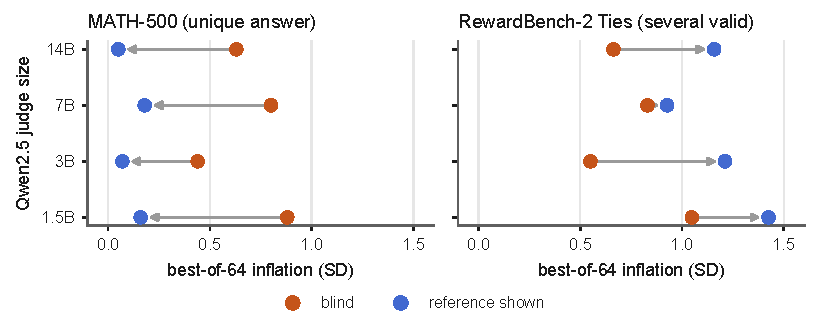
\includegraphics[width=\textwidth]{figures/figA_inversion.pdf}
\caption{\textbf{Showing the reference lowers inflation on MATH-500 and raises it on Ties.} Best-of-64 inflation for blind (orange) and referenced (blue) Qwen2.5 judges, 105 MATH-500 problems and 51 Ties tasks.}
\label{fig:inversion}
\end{figure}

In accuracy units, the reference raises MATH-500 selection accuracy at every judge size (\cref{tab:acc-math}). The local copies of these MATH-500 score files that we first used for this readout were misaligned with the candidate pool; all MATH-500 analyses reported here use byte-exact copies of the aligned files, as recorded in a registration amendment made before the remaining readouts.

\begin{table}[htbp]
\centering
\caption{MATH-500 selection accuracy, 105 problems (95\% CI on the change).\ph}
\label{tab:acc-math}
\footnotesize
\begin{adjustbox}{max width=\linewidth}\begin{tabular}{lccc}
\toprule
Qwen2.5 judge & Blind & With reference & Change (points) \\
\midrule
1.5B & 55.2\% & 99.1\% & $+43.8$ {\scriptsize$[+34.3,+53.3]$} \\
3B & 57.1\% & 96.2\% & $+39.1$ {\scriptsize$[+30.5,+48.6]$} \\
7B & 67.6\% & 98.1\% & $+30.5$ {\scriptsize$[+21.9,+40.0]$} \\
14B & 67.6\% & 95.2\% & $+27.6$ {\scriptsize$[+18.1,+37.1]$} \\
\bottomrule
\end{tabular}
\end{adjustbox}

\end{table}

%==========================================================================================
\FloatBarrier
\section{A pilot on combinatorial constraint problems}
\label{app:mathconstraint}

Our own pools come from arithmetic constraint families. To check whether swap and margins depend on that, we ran a pre-specified pilot on MathConstraint~\citep{mathconstraint2026}, a third-party benchmark of solver-verified combinatorial puzzles. Llama-3.1-8B-Instruct and Qwen2.5-32B-Instruct (with a worked example) solved none of 8 attempts past the smallest size, so a Claude model generated candidate solutions, each re-verified with exact checkers. It solved all 13 attempted items. Magic sequences turned out to be essentially unique past the smallest size, so the tests use all-interval series, which have several solutions at every size tried.

Rotating the reference between two valid solutions moves a fixed candidate by $+3.46$ \ci{+2.71}{+4.09} and $+3.93$ \ci{+3.42}{+4.40} for Qwen2.5-7B (rubrics $a$, $b$) and $+5.01$ \ci{+4.38}{+5.54} and $+3.90$ \ci{+3.27}{+4.49} for phi-4, and the margin is positive on all 9 eligible items for both judges. A follow-up used all six pairs of valid answers per item: $+3.21$ \ci{+2.92}{+3.51} and $+3.53$ \ci{+3.27}{+3.81} for Qwen2.5-7B and $+5.04$ \ci{+4.79}{+5.28} and $+4.10$ \ci{+3.84}{+4.36} for phi-4 (96 observations each). An invalid answer that differs from the reference by one adjacent swap scores higher than an unrelated invalid answer by $+3.47$ \ci{+2.31}{+4.52} and $+1.42$ \ci{+0.77}{+2.14}. Sonnet~5 shows the swap ($+4.38$ \ci{+1.88}{+6.88}) and a margin of $+6.41$ \ci{+3.70}{+8.74}.

Five pre-specified attempts tested selection on this domain. The first two failed for diagnosed reasons: mixing a few valid solutions into many obviously broken attempts recreated the unique-answer case, and replacing the broken attempts with a second valid solution ran into a solution so regular that judges preferred it even blind. The third used two unstructured valid solutions and a near-miss invalid variant of each, and also failed: with the reference shown, both judges picked the candidate identical to the reference in all 16 cases. In all three designs the reference's own text was one of the candidates, so its top score shows only that a judge recognizes the string it was shown. The fourth attempt removed that candidate and asked whether showing one valid solution as the reference makes judges prefer a near-miss variant of it over a different valid solution. Both judges moved in the predicted direction (the valid pick rate fell from 0.625 to 0.375 for Qwen2.5-7B and from 0.500 to 0.375 for phi-4), but with 8 items neither interval excludes zero. A fifth attempt, registered before any new judging, doubled the paired comparisons to 16 by adding each instance's fourth valid solution against the same near-miss variant, and pooled them with the fourth attempt's. The valid pick rate fell from 0.562 to 0.250 for Qwen2.5-7B (paired difference $-0.31$ \ci{-0.56}{-0.13}) and from 0.500 to 0.375 for phi-4 ($-0.13$ \ci{-0.31}{0.00}): confirmed for Qwen2.5-7B and not confirmed for phi-4, a split verdict on 16 comparisons from 8 items.
%==========================================================================================
\FloatBarrier
\section{Code and the answer-format continuum}
\label{app:code}

We registered the prediction that MBPP's canonical program, shown as the reference, would add inflation the way a stated answer does, while a test suite would not. It was falsified: the canonical program did not add inflation ($-0.34$ \ci{-0.74}{+0.04} and $-0.57$~\sd{} for the 7B and 14B judges), and neither did the test suite (\cref{tab:code}). Asking the same constraint questions in four answer formats, the added inflation fell from integer to pair, JSON, and program ($+1.66 \to +0.13$ for Qwen2.5-7B, $+1.35 \to -0.37$ for phi-4), although the margin on programs stayed positive ($+0.64$ and $+0.88$). Program outputs have few distinct correct values per task, so this decline cannot be separated from a smaller effective $k$.

\paragraph{MBPP.}
Three conditions score identical samples with identical judges: blind, the test suite as reference, and the canonical solution as reference. Contrasts use the 58 tasks inside the pass-rate band shared by all three.

\begin{table}[htbp]
\centering
\caption{MBPP: paired inflation differences (\sd, 95\% CI), 58 tasks. Negative values mean the reference lowers inflation.\pre}
\label{tab:code}
\footnotesize
\begin{tabular}{lccc}
\toprule
Judge & Test suite vs.\ blind & Canonical solution vs.\ blind & Solution minus test suite \\
\midrule
Qwen2.5-7B  & $-0.535$ \ci{-0.811}{-0.244} & $-0.342$ \ci{-0.737}{+0.041} & $+0.193$ \ci{-0.112}{+0.475} \\
Qwen2.5-14B & $-0.658$ \ci{-0.965}{-0.373} & $-0.567$ \ci{-0.827}{-0.287} & $+0.091$ \ci{-0.102}{+0.277} \\
\bottomrule
\end{tabular}

\end{table}

Among valid samples, the correlation between token similarity to the canonical solution and the judge's score is $+0.164$ \ci{+0.072}{+0.256} for the 7B judge and $+0.084$ \ci{-0.005}{+0.168} for the 14B judge with the solution shown, against $-0.061$ and $-0.070$ blind.

\paragraph{The continuum.}
Each of 25 new tasks was requested in four formats with the content fixed. Three disclosures apply. The margin predictions at the pair and JSON formats could not be evaluated, because a valid sample rarely matches the sampled reference exactly in those formats (7 and 1 usable tasks). Program outputs cluster (a median of two distinct returned lists per task), so the program format has few distinct valid answers. And the registered program checker executed the last code block of a reply, which scored 387 of 1,600 samples invalid when a usage line such as \texttt{print(f())} followed the definition of \texttt{f}; re-scoring with the last block that defines \texttt{f} flipped 330 of them to valid and none the other way. \Cref{tab:continuum} uses the corrected labels. Under the registered labels the program-format values were $+0.27$ \ci{+0.13}{+0.40} and $-0.06$ \ci{-0.22}{+0.11}; no registered verdict changes.

\begin{table}[htbp]
\centering
\caption{Answer-format continuum: added inflation (\sd, 95\% CI) and margins with the number of usable tasks; margins on fewer than five tasks are omitted.\pre}
\label{tab:continuum}
\footnotesize
\setlength{\tabcolsep}{3pt}
\begin{adjustbox}{max width=\linewidth}\begin{tabular}{llcccc}
\toprule
Judge & Readout & Integer & Pair & JSON & Program \\
\midrule
Qwen2.5-7B & added inflation ($n{=}25$) & $+1.66$ {\scriptsize$[+1.34,+2.03]$} & $+1.35$ {\scriptsize$[+1.06,+1.68]$} & $+0.71$ {\scriptsize$[+0.40,+1.02]$} & $+0.13$ {\scriptsize$[+0.01,+0.24]$} \\
 & margin & $+4.65$ {\scriptsize($n{=}17$)} & $+5.45$ {\scriptsize($n{=}7$)} & --- {\scriptsize($n{=}1$)} & $+0.64$ {\scriptsize($n{=}19$)} \\
phi-4 & added inflation ($n{=}25$) & $+1.35$ {\scriptsize$[+1.06,+1.65]$} & $+0.98$ {\scriptsize$[+0.77,+1.21]$} & $+0.94$ {\scriptsize$[+0.56,+1.30]$} & $-0.37$ {\scriptsize$[-0.49,-0.27]$} \\
 & margin & $+3.22$ {\scriptsize($n{=}17$)} & $+3.79$ {\scriptsize($n{=}7$)} & --- {\scriptsize($n{=}1$)} & $+0.88$ {\scriptsize($n{=}19$)} \\
\bottomrule
\end{tabular}
\end{adjustbox}

\end{table}

\begin{figure}[htbp]
\centering
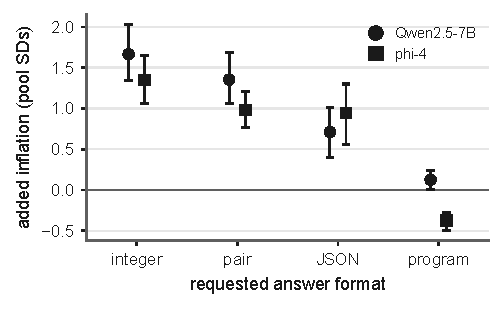
\includegraphics[width=0.55\textwidth]{figures/figA_continuum.pdf}
\caption{\textbf{Answer format.} Added best-of-64 inflation when the same content is requested as an integer, a pair, a JSON object, or a Python program whose output is checked (25 tasks). Both judges' program values use the corrected checker labels; program outputs have few distinct correct answers.\pre}
\label{fig:continuum}
\end{figure}

%==========================================================================================
\FloatBarrier
\section{Training runs}
\label{app:dpo}

Arms trained Llama-3.1-8B-Instruct with LoRA-DPO~\citep{rafailov2023dpo,hu2022lora} on identical tasks and hyperparameters, differing only in the judge protocol that labeled the preference pairs: the referenced Qwen2.5-7B judge, the same judge under blind-then-reveal, and in run 3 the blind judge. Each arm's manipulation check required its own judge's score to rise. The \emph{score--accuracy gap} is the rise in own-judge score (points) minus ten times the rise in accuracy, so both terms are on the 0--10 scale.

\begin{table}[htbp]
\centering
\caption{Training runs. Only the reference arm passed its manipulation check. Run 2 (1 epoch, lr $5{\times}10^{-6}$) moved neither judge and is omitted.\pre}
\label{tab:dpo}
\footnotesize
\setlength{\tabcolsep}{3pt}
\begin{adjustbox}{max width=\linewidth}\begin{tabular}{llccc}
\toprule
Run & Arm & Own-judge gain (gate) & Score--accuracy gap (points) & Held-out accuracy change \\
\midrule
1 (4 ep., lr $2{\times}10^{-5}$) & reference & \begin{tabular}[c]{@{}c@{}}$+1.76$\\{\scriptsize$[+1.47,+2.01]$}\end{tabular} & \begin{tabular}[c]{@{}c@{}}$+4.13$\\{\scriptsize$[+3.50,+4.78]$}\end{tabular} & \begin{tabular}[c]{@{}c@{}}$-0.228$\\{\scriptsize$[-0.269,-0.189]$}\end{tabular} \\
 & blind-then-reveal & \begin{tabular}[c]{@{}c@{}}$-1.04$\\{\scriptsize$[-1.36,-0.72]$}\end{tabular} & \begin{tabular}[c]{@{}c@{}}$+1.48$\\{\scriptsize$[+0.99,+1.97]$}\end{tabular} & \begin{tabular}[c]{@{}c@{}}$-0.049$\\{\scriptsize$[-0.091,-0.010]$}\end{tabular} \\
\addlinespace
3 (2 ep., lr $10^{-5}$) & reference & \begin{tabular}[c]{@{}c@{}}$+0.34$\\{\scriptsize$[+0.10,+0.57]$}\end{tabular} & \begin{tabular}[c]{@{}c@{}}$+1.16$\\{\scriptsize$[+0.67,+1.61]$}\end{tabular} & \begin{tabular}[c]{@{}c@{}}$-0.110$\\{\scriptsize$[-0.149,-0.074]$}\end{tabular} \\
 & blind-then-reveal & \begin{tabular}[c]{@{}c@{}}$-0.99$\\{\scriptsize$[-1.23,-0.74]$}\end{tabular} & \begin{tabular}[c]{@{}c@{}}$+1.10$\\{\scriptsize$[+0.62,+1.58]$}\end{tabular} & \begin{tabular}[c]{@{}c@{}}$-0.073$\\{\scriptsize$[-0.107,-0.040]$}\end{tabular} \\
 & blind judge & \begin{tabular}[c]{@{}c@{}}$-2.43$\\{\scriptsize$[-2.78,-2.12]$}\end{tabular} & \begin{tabular}[c]{@{}c@{}}$+1.90$\\{\scriptsize$[+1.41,+2.43]$}\end{tabular} & \begin{tabular}[c]{@{}c@{}}$-0.125$\\{\scriptsize$[-0.159,-0.092]$}\end{tabular} \\
\bottomrule
\end{tabular}
\end{adjustbox}

\end{table}

The reference arm did not copy the reference more often; its exact-reference rate fell. It wrote longer answers and mostly stopped using the boxed format, and almost all of its unboxed answers were also wrong (390 of 405 on training tasks), so this is a joint failure of format and correctness, not an extraction artifact (\cref{tab:dpo-profile}). Held-out accuracy fell in every arm, including the controls. In run 1 both arms drifted toward verbosity, which the blind-first judge penalizes; in run 2 neither arm moved; before run 3 we adopted a stopping rule allowing one more setting, and in run 3 the reveal and blind arms lost score and accuracy together. We stopped there, so whether blind-then-reveal protects a trained policy, and whether the reference specifically causes the damage, remain open.

\begin{table}[htbp]
\centering
\caption{Generation profile of the run-1 policies.\ph}
\label{tab:dpo-profile}
\scriptsize
\setlength{\tabcolsep}{3pt}
\begin{adjustbox}{max width=\linewidth}\begin{tabular}{lcccccc}
\toprule
Policy (items) & Accuracy & Boxed answers & Mean length (chars) & 4-gram repetition & Unboxed and valid & Unboxed and invalid \\
\midrule
Base, train (60) & 0.412 & 0.581 & 1492 & 0.080 & 3 & 198 \\
Reference arm, train (60) & 0.175 & 0.156 & 2476 & 0.062 & 15 & 390 \\
Reveal arm, train (60) & 0.331 & 0.365 & 3840 & 0.032 & 0 & 305 \\
Base, held out (120) & 0.457 & 0.613 & 1376 & 0.080 & 13 & 359 \\
Reference arm, held out (120) & 0.229 & 0.174 & 2187 & 0.064 & 57 & 736 \\
Reveal arm, held out (120) & 0.408 & 0.455 & 3458 & 0.041 & 4 & 519 \\
\bottomrule
\end{tabular}
\end{adjustbox}

\end{table}



\bibliography{references}
\bibliographystyle{iclr2027_conference}

\end{document}
